\documentclass[a4paper]{article}
\usepackage{graphicx}

\usepackage[  margin=2.5cm,  includefoot,  footskip=30pt,]{geometry}

%\usepackage[cm]{fullpage}
\usepackage{bm}
\usepackage{listings}
\usepackage{amsmath}
\usepackage{amsfonts}
\usepackage{hyperref}
%\usepackage{xcolor}
\usepackage{mdframed}
\usepackage{makeidx} 
\usepackage{xargs}
\usepackage[pdftex,dvipsnames]{xcolor}
\usepackage[colorinlistoftodos,prependcaption,textsize=tiny]{todonotes}
\hypersetup{
    colorlinks,
    citecolor=black,
    filecolor=black,
    linkcolor=black,
    urlcolor=black
}
\lstset{ 
  language=Python,
  backgroundcolor=\color{white},   % choose the background color; you must add \usepackage{color} or \usepackage{xcolor}; should come as last argument
  basicstyle=\footnotesize,        % the size of the fonts that are used for the code
  breakatwhitespace=false,         % sets if automatic breaks should only happen at whitespace
  breaklines=true,                 % sets automatic line breaking
  captionpos=b,                    % sets the caption-position to bottom
  frame=single,                    % adds a frame around the code
  keepspaces=true,                 % keeps spaces in text, useful for keeping indentation of code (possibly needs columns=flexible)
  keywordstyle=\color{blue},       % keyword style
}

\newcommand{\nn}{\nonumber}
\newcommand{\A}{{\mathbb{A}}}
\newcommand{\K}{{\mathbb{K}}}
\newcommand{\G}{{\mathbb{G}}}
\newcommand{\Z}{{\mathbb{Z}}}
\newcommand{\C}{{\mathbb{C}}}
\newcommand{\W}{{\mathbb{W}}}
\newcommand{\LLL}{{\mathbb{L}}}
\newcommand{\SSS}{{\mathbb{S}}}
\newcommand{\fieldstone}{{\bf fieldstone}}

\newcommandx{\unsure}[2][1=]{\todo[linecolor=red,backgroundcolor=red!25,bordercolor=red,#1]{#2}}
\newcommandx{\change}[2][1=]{\todo[linecolor=blue,backgroundcolor=blue!25,bordercolor=blue,#1]{#2}}
\newcommandx{\info}[2][1=]{\todo[linecolor=OliveGreen,backgroundcolor=OliveGreen!25,bordercolor=OliveGreen,#1]{#2}}
\newcommandx{\improvement}[2][1=]{\todo[linecolor=Plum,backgroundcolor=Plum!15,bordercolor=Plum,#1]{#2}}
\newcommandx{\thiswillnotshow}[2][1=]{\todo[disable,#1]{#2}}

%%%%%%%%%%%%%%%%%%%%%%%%%%%%%%%%%%%%%%%%%%%%%%%%%%%%%%%%%%%%%%%%%%%%%%%%%%%%%%%%%%%%%%%%%%%%%%%%%%%
%%%%%%%%%%%%%%%%%%%%%%%%%%%%%%%%%%%%%%%%%%%%%%%%%%%%%%%%%%%%%%%%%%%%%%%%%%%%%%%%%%%%%%%%%%%%%%%%%%%
%%%%%%%%%%%%%%%%%%%%%%%%%%%%%%%%%%%%%%%%%%%%%%%%%%%%%%%%%%%%%%%%%%%%%%%%%%%%%%%%%%%%%%%%%%%%%%%%%%%
%%%%%%%%%%%%%%%%%%%%%%%%%%%%%%%%%%%%%%%%%%%%%%%%%%%%%%%%%%%%%%%%%%%%%%%%%%%%%%%%%%%%%%%%%%%%%%%%%%%
%%%%%%%%%%%%%%%%%%%%%%%%%%%%%%%%%%%%%%%%%%%%%%%%%%%%%%%%%%%%%%%%%%%%%%%%%%%%%%%%%%%%%%%%%%%%%%%%%%%

\title{The Finite Element Method in Geodynamics}

\author{C. Thieulot}

\makeindex 
\begin{document}

\maketitle

\tableofcontents

\newpage

\begin{center}
{\color{red} \huge WARNING: this is work in progress}
\end{center}

%%%%%%%%%%%%%%%%%%%%%%
\section{Introduction}

\subsection{Philosophy} %------------------------------------------------------
This document was writing with my students in mind, i.e. 3rd and 4th year 
Geology/Geophysics students at Utrecht University. 
I have chosen to use jargon as little as possible unless it is a term that is 
commonly found in the geodynamics literature (methods paper as well as 
application papers). There is no mathematical proof of any theorem or statement 
I make. These are to be found in generic Numerical Analysic, Finite Element and 
Linear Algebra books. 

The codes I provide here are by no means optimised as I value code readability 
over code efficiency. I have also chosen to avoid resorting to multiple code 
files or even functions to favour a sequential reading of the codes. 
These codes are not designed to form the basis of a real life application:
Existing open source highly optimised codes shoud be preferred, such as ASPECT, 
CITCOM, LAMEM, PTATIN, PYLITH, ... 

All kinds of feedback is welcome on the text (grammar, typos, ...) or on the 
code(s). You will have my eternal gratitude if you wish to contribute an 
example, a benchmark, a cookbook. 

All the python scripts and this document are freely available at 
\begin{center}
\url{https://github.com/cedrict/fieldstone}
\end{center}

\subsection{Acknowledgments} %-------------------------------------------------

I have benefitted from many discussions, lectures, tutorials, coffee machine 
discussions, debugging sessions, conference poster sessions, etc ... 
over the years. I wish to name these instrumental people in particular and 
in alphabetic order: 
Wolfgang Bangerth, 
Jean Braun, 
Philippe Fullsack, 
Menno Fraters, 
Anne Glerum,
Timo Heister,
Robert Myhill,
John Naliboff,
Lukas van de Wiel,
Arie van den Berg, and the whole ASPECT family/team. 

I wish to acknowledge many BSc and MSc students for their questions and feedback.
and wish to mention Job Mos in particular who wrote the
very first version of fieldstone as part of his MSc thesis.
and Tom Weir for his contributions to the compressible formulations.



\subsection{Essential literature} %--------------------------------------------

\begin{center}
\includegraphics[height=3.74cm]{images/literature/gerya_book}
\includegraphics[height=3.74cm]{images/literature/tackley_book}
\includegraphics[height=3.74cm]{images/literature/donea_huerta_book}
\includegraphics[height=3.74cm]{images/literature/bercovici_book}
\includegraphics[height=3.74cm]{images/literature/sto_book}\\
\end{center}

%---------------------------------------
\subsection{Installation}

\begin{verbatim}
python3.6 -m pip install --user numpy scipy matplotlib
\end{verbatim}

\newpage
%%%%%%%%%%%%%%%%%%%%%%%%%%%%%%%%%%%%%%%%%%%%%%%%%%%%%%%%%%%%%%%%%%%%%%%%%%%%%%%
\section{The physical equations of Fluid Dynamics} %%%%%%%%%%%%%%%%%%%%%%%%%%%% 
\input{physics}

\newpage
%%%%%%%%%%%%%%%%%%%%%%%%%%%%%%%%%%%%%%%%%%%%%%%%%%%%%%%%%%%%%%%%%%%%%%%%%%%%%%%
\section{The building blocks of the Finite Element Method} %%%%%%%%%%%%%%%%%%%%

\subsection{Numerical integration} \input{quadrature} %------------------------

\subsection{The mesh}

\subsection{A bit of FE terminology} \input{terminology} %---------------------

\subsection{Elements and basis functions in 1D} \input{elements1D} %-----------

\subsection{Elements and basis functions in 2D} \input{elements} %-------------

\newpage 
%%%%%%%%%%%%%%%%%%%%%%%%%%%%%%%%%%%%%%%%%%%%%%%%%%%%%%%%%%%%%%%%%%%%%%%%%%%%%%%
\section{Solving the Stokes equations with the FEM} %%%%%%%%%%%%%%%%%%%%%%%%%%%
\input{incompressible} %-------------------------------------------------------

\subsection{strong and weak forms} \input{strongweak} %------------------------

\subsection{The penalty approach} \input{penalty} %----------------------------

\subsection{The mixed FEM} \input{mixed} %-------------------------------------



\newpage
%%%%%%%%%%%%%%%%%%%%%%%%%%%%%%%%%%%%%%%%%%%%%%%%%%%%%%%%%%%%%%%%%%%%%%%%%%%%%%%
\section{Solving the elastic equations with the FEM}




%\subsection{Solving procedures}

%\subsubsection{the whole matrix at once}

%\subsubsection{the pressure Schur complement appraoch}



\newpage
%%%%%%%%%%%%%%%%%%%%%%%%%%%%%%%%%%%%%%%%%%%%%%%%%%%%%%%%%%%%%%%%%%%%%%%%%%%%%%%
\section{Additional techniques} %%%%%%%%%%%%%%%%%%%%%%%%%%%%%%%%%%%%%%%%%%%%%%%

\subsection{Picard and Newton}

\subsection{The SUPG formulation for the energy equation}

\subsection{Tracking materials and/or interfaces}

\subsection{Dealing with a free surface}

\subsection{Convergence criterion for nonlinear iterations}

\subsection{Static condensation} \index{static condensation}

\newpage %---------------------------------------------------------------------
\subsection{The method of manufactured solutions} \input{mms} %----------------

\newpage %---------------------------------------------------------------------
\subsection{Assigning values to quadrature points} \input{averagings} %--------

\newpage %---------------------------------------------------------------------
\subsection{Matrix (Sparse) storage} \input{storage} %-------------------------

\newpage %---------------------------------------------------------------------
\subsection{Mesh generation} \label{subsection_meshes} \input{meshes} %--------

\newpage %---------------------------------------------------------------------
\subsection{Visco-Plasticity} \input{viscoplasticity} %------------------------

\newpage %---------------------------------------------------------------------
\subsection{Pressure smoothing} \input{pressure_smoothing} %-------------------

\newpage %---------------------------------------------------------------------
\subsection{Pressure scaling} \input{pressure_scaling} %-----------------------

\newpage %---------------------------------------------------------------------
\subsection{Pressure normalisation} \input{pressure_normalisation} %----------

\newpage %---------------------------------------------------------------------
\subsection{The choice of solvers\label{sec_solvers}} \input{solvers} %--------

\newpage %---------------------------------------------------------------------
\subsection{The consistent boundary flux (CBF)} The Consistent Boundary Flux technique was devised to 
alleviate the problem of the accuracy of primary variables 
derivatives (mainly velocity and temperature) on boundaries, 
where basis function (nodal) derivatives do not exist.
These derivatives are important since they are needed to compute
the heat flux (and therefore the NUsselt number) or 
dynamic topography and geoid. 


The idea was first introduced in \cite{mizu86} and later used 
in geodynamics \cite{zhgh93}. It was finally implemented 
in the CitcomS code \cite{zhmt08} and more recently
in the ASPECT code (dynamic topography postprocessor).
Note that the CBF should be seen as a post-processor step 
as it does not alter the primary variables values.

The CBF method is implemented and used in \ref{f_XX}.

%---------------------------------------------------------------
\subsubsection{applied to the Stokes equation}
We start from the strong form:
\[
{\bm \nabla}\cdot{\bm \sigma} = {\bm b}
\]
and then write the weak form:
\[
\int_\Omega N {\bm \nabla}\cdot{\bm \sigma} dV = \int_\Omega N {\bm b} dV
\]
where $N$ is any test function. We then use the two equations:
\[
\bm \nabla \cdot ( N  \bm \sigma ) = N \bm \nabla \cdot \bm \sigma + \bm \nabla N \cdot  \bm \sigma  
\quad\quad \text{(chain rule)}
\]
\[
\int_\Omega (\bm \nabla \cdot \bm f )\; dV = \int_\Gamma \bm f\cdot \bm n \; dS
\quad\quad \text{(divergence theorem)}
\]
Integrating the first equation over $\Omega$ and using the second, we can write:
\[
\int_\Gamma N {\bm \sigma}\cdot {\bm n} \; dS 
-  \int_\Omega {\nabla N} \cdot{\bm \sigma} \; dV 
= \int_\Omega N {\bm b} dV
\]
On $\Gamma$, the traction vector is given by ${\bm t}={\bm \sigma}\cdot {\bm n}$: 
\[
\int_\Gamma N {\bm t} dS =  \int_\Omega {\nabla N} \cdot{\bm \sigma} dV + \int_\Omega N {\bm b} dV
\]
Considering the traction vector as an unknown living on the nodes on the boundary, 
we can expand (for $Q_1$ elements)
\[
t_x = \sum_{i=1}^2 t_{x|i} N_i 
\quad\quad
t_y = \sum_{i=1}^2 t_{y|i} N_i 
\]
on the boundary so that the left hand term yields a mass matrix $M'$.
Finally, using our previous experience of discretising the weak form, we can write:
\[
M' \cdot {\cal T} = -\K {\cal V} - \G {\cal P} + f
\]
where ${\cal T}$ is the vector of assembled tractions which we want to compute 
and ${\cal V}$ and ${\cal T}$ are the solutions of the Stokes problem. 
Note that the assembly
only takes place on the elements along the boundary.

Note that the assembled mass matrix is tri-diagonal can be easily solved with 
a Conjugate Gradient method. With a trapezoidal integration rule 
(i.e. Gauss-Lobatto) the matrix can even be diagonalised and the resulting 
matrix is simply diagonal, which results in a very cheap solve \cite{zhgh93}.

%---------------------------------------------------------------
\subsubsection{applied to the heat equation}
We start from the strong form of the heat transfer equation (without the source terms for simplicity):
\[
\rho c_p
\left(\frac{\partial T}{\partial t} + {\bm v}\cdot {\bm \nabla}T\right)
=
{\bm \nabla} \cdot k{\bm \nabla T}
\]
The weak form then writes:
%\[
%\int_\Omega N
%\rho c_p
%\left(\frac{\partial T}{\partial t} + {\bm v}\cdot {\bm \nabla}T\right) dV
%=
%\int_\Omega N
%{\bm \nabla} \cdot k{\bm \nabla T} dV
%\]
\[
\int_\Omega N
\rho c_p
\frac{\partial T}{\partial t} dV 
+
\rho c_p
\int_\Omega N
 {\bm v}\cdot {\bm \nabla}T  dV
=
\int_\Omega N
{\bm \nabla} \cdot k{\bm \nabla T} dV
\]
Using once again integration by parts and divergence theorem:
\[
\int_\Omega N
\rho c_p
\frac{\partial T}{\partial t} dV 
+
\rho c_p
\int_\Omega N
 {\bm v}\cdot {\bm \nabla}T  dV
=
\int_\Gamma N k {\bm \nabla T} \cdot {\bm n} d\Gamma
-
\int_\Omega  {\bm \nabla} N \cdot k{\bm \nabla T} dV
\]
On the boundary we are interested in the heat flux ${\bm q}=-k {\bm \nabla T}$
\[
\int_\Omega N
\rho c_p
\frac{\partial T}{\partial t} dV 
+
\rho c_p
\int_\Omega N
 {\bm v}\cdot {\bm \nabla}T  dV
=
-\int_\Gamma N {\bm q} \cdot {\bm n} d\Gamma
- \int_\Omega  {\bm \nabla} N \cdot k{\bm \nabla T} dV
\]
or,
\[
\int_\Gamma N {\bm q} \cdot {\bm n} d\Gamma
=
-\int_\Omega N
\rho c_p
\frac{\partial T}{\partial t} dV 
-\rho c_p
\int_\Omega N
 {\bm v}\cdot {\bm \nabla}T  dV
- \int_\Omega  {\bm \nabla} N \cdot k{\bm \nabla T} dV
\]
Considering the normal heat flux $q_n = {\bm q} \cdot {\bm n}$ as an unknown 
living on the nodes on the boundary, 
\[
q_n = \sum_{i=1}^2 q_{n|i} N_i
\]
so that the left hand term becomes a mass matrix for the shape functions living on 
the boundary.
We have already covered the right hand side terms when building the FE system 
to solve the heat transport equation, so that in the end 
\[
M' \cdot {\cal Q}_n =
- M \cdot \frac{\partial \bm T}{\partial t} -K_a \cdot {\bm T} - K_d \cdot {\bm T} 
\]
where ${\cal Q}_n$ is the assembled vector of normal heat flux components.

Note that in all terms the assembly only takes place over the elements along the boundary.







\newpage
What follows only applies to the reference element.

\begin{verbatim}
    N
 3-----2
 |     |
W|     |E
 |     |
 0-----1
    S
\end{verbatim}

We start from 
\begin{eqnarray}
\int_{\Gamma} N_i {\bm t} dS 
&=& 
 \int_{\Gamma_{0-1}} N_i {\bm t} dS  
+\int_{\Gamma_{1-2}} N_i {\bm t} dS  
+\int_{\Gamma_{2-3}} N_i {\bm t} dS  
+\int_{\Gamma_{3-0}} N_i {\bm t} dS
\end{eqnarray}
for $i=0,3$. Let us start with $N_0$, then 

\begin{eqnarray}
\int_{\Gamma} N_0 {\bm t} dS 
&=& 
 \int_{\Gamma_{0-1}} N_0 {\bm t} dS  
+\int_{\Gamma_{1-2}} N_0 {\bm t} dS  
+\int_{\Gamma_{2-3}} N_0 {\bm t} dS  
+\int_{\Gamma_{3-0}} N_0 {\bm t} dS \nn\\
&=& \int_{\Gamma_{0-1}} N_0 (N_0^\Gamma {\bm t}_0 + N_1^\Gamma {\bm t}_1) dS \nn\\ 
&+& \int_{\Gamma_{1-2}} N_0 (N_1^\Gamma {\bm t}_1 + N_2^\Gamma {\bm t}_2) dS \nn\\
&+& \int_{\Gamma_{2-3}} N_0 (N_2^\Gamma {\bm t}_2 + N_3^\Gamma {\bm t}_3) dS \nn\\
&+& \int_{\Gamma_{3-0}} N_0 (N_3^\Gamma {\bm t}_3 + N_0^\Gamma {\bm t}_0) dS \nn\\ 
&=& \left( \int_{\Gamma_{0-1}} N_0 N_0^\Gamma dS \right) {\bm t}_0 + \left( \int_{\Gamma_{0-1}} N_0 N_1^\Gamma dS\right) {\bm t}_1 \nn\\ 
&+& \left( \int_{\Gamma_{1-2}} N_0 N_1^\Gamma dS \right) {\bm t}_1 + \left( \int_{\Gamma_{1-2}} N_0 N_2^\Gamma dS\right) {\bm t}_2 \nn\\
&+& \left( \int_{\Gamma_{2-3}} N_0 N_2^\Gamma dS \right) {\bm t}_2 + \left( \int_{\Gamma_{2-3}} N_0 N_3^\Gamma dS\right) {\bm t}_3 \nn\\
&+& \left( \int_{\Gamma_{3-0}} N_0 N_3^\Gamma dS \right) {\bm t}_3 + \left( \int_{\Gamma_{3-0}} N_0 N_0^\Gamma dS\right) {\bm t}_0 \nn  
\end{eqnarray}

In what follows we will make use of 
\[
\int_{-1}^{+1} \frac{1}{4} (1-x)(1-x) dx = 2/3 
\]
\[
\int_{-1}^{+1} \frac{1}{4} (1+x)(1+x) dx = 2/3 
\]
\[
\int_{-1}^{+1} \frac{1}{4} (1+x)(1-x) dx = 1/3 
\]



\newpage 
\begin{eqnarray}
\int_{\Gamma_{0-1}} N_0(r,s=-1) N_0^\Gamma(r) dS  &=&  \int_{-1}^{+1}\frac{1}{2}(1-r) \cdot  \frac{1}{2}(1-r) dr= 2/3 \nn\\
\int_{\Gamma_{0-1}} N_0(r,s=-1) N_1^\Gamma(r) dS  &=&  \int_{-1}^{+1}\frac{1}{2}(1-r) \cdot  \frac{1}{2}(1+r) dr= 1/3 \nn\\
\int_{\Gamma_{1-2}} N_0(r=+1,s) N_1^\Gamma(s) dS  &=&  \int_{-1}^{+1}\frac{1}{4}(0)(1-s) \cdot  \frac{1}{2}(1-s) ds=0 \nn\\
\int_{\Gamma_{1-2}} N_0(r=+1,s) N_2^\Gamma(s) dS  &=&  \int_{-1}^{+1}\frac{1}{4}(0)(1-s) \cdot  \frac{1}{2}(1+s) ds=0 \nn\\
\int_{\Gamma_{2-3}} N_0(r,s=+1) N_2^\Gamma(r) dS  &=&  -\int_{-1}^{+1}\frac{1}{4}(1-r)(0) \cdot  \frac{1}{2}(1+r) dr=0 \nn\\
\int_{\Gamma_{2-3}} N_0(r,s=+1) N_3^\Gamma(r) dS  &=&  -\int_{-1}^{+1}\frac{1}{4}(1-r)(0) \cdot  \frac{1}{2}(1-r) dr=0 \nn\\
\int_{\Gamma_{3-0}} N_0(r=-1,s) N_3^\Gamma(s) dS  &=&  -\int_{-1}^{+1}\frac{1}{2}(1-s) \cdot  \frac{1}{2}(1+s) ds= -1/3 \nn\\
\int_{\Gamma_{3-0}} N_0(r=-1,s) N_0^\Gamma(s) dS  &=&  -\int_{-1}^{+1}\frac{1}{2}(1-s) \cdot  \frac{1}{2}(1-s) ds= -2/3 \nn
\end{eqnarray}

\begin{eqnarray}
\int_{\Gamma_{0-1}} N_1(r,s=-1) N_0^\Gamma(r) dS  &=&  \int_{-1}^{+1} \frac{1}{2}(1+r)     \cdot  \frac{1}{2}(1-r) dr= 1/3\nn\\
\int_{\Gamma_{0-1}} N_1(r,s=-1) N_1^\Gamma(r) dS  &=&  \int_{-1}^{+1} \frac{1}{2}(1+r)     \cdot  \frac{1}{2}(1+r) dr= 2/3\nn\\
\int_{\Gamma_{1-2}} N_1(r=+1,s) N_1^\Gamma(s) dS  &=&  \int_{-1}^{+1} \frac{1}{2}(1-s)     \cdot  \frac{1}{2}(1-s) ds= 2/3\nn\\
\int_{\Gamma_{1-2}} N_1(r=+1,s) N_2^\Gamma(s) dS  &=&  \int_{-1}^{+1} \frac{1}{2}(1-s)     \cdot  \frac{1}{2}(1+s) ds= 1/3\nn\\
\int_{\Gamma_{2-3}} N_1(r,s=+1) N_2^\Gamma(r) dS  &=&  -\int_{-1}^{+1}\frac{1}{4}(1+r)(0)  \cdot  \frac{1}{2}(1+r) dr= 0\nn\\
\int_{\Gamma_{2-3}} N_1(r,s=+1) N_3^\Gamma(r) dS  &=&  -\int_{-1}^{+1}\frac{1}{4}(1+r)(0)  \cdot  \frac{1}{2}(1-r) dr= 0\nn\\
\int_{\Gamma_{3-0}} N_1(r=-1,s) N_3^\Gamma(s) dS  &=&  -\int_{-1}^{+1}\frac{1}{4}(0)(1-s)  \cdot  \frac{1}{2}(1+s) ds= 0\nn\\
\int_{\Gamma_{3-0}} N_1(r=-1,s) N_0^\Gamma(s) dS  &=&  -\int_{-1}^{+1}\frac{1}{4}(0)(1-s)  \cdot  \frac{1}{2}(1-s) ds= 0\nn
\end{eqnarray}

\begin{eqnarray}
\int_{\Gamma_{0-1}} N_2(r,s=-1) N_0^\Gamma(r) dS  &=&  \int_{-1}^{+1} \frac{1}{4}(1+r)(0)  \cdot  \frac{1}{2}(1-r) dr= 0\nn\\
\int_{\Gamma_{0-1}} N_2(r,s=-1) N_1^\Gamma(r) dS  &=&  \int_{-1}^{+1} \frac{1}{4}(1+r)(0)  \cdot  \frac{1}{2}(1+r) dr= 0\nn\\
\int_{\Gamma_{1-2}} N_2(r=+1,s) N_1^\Gamma(s) dS  &=&  \int_{-1}^{+1} \frac{1}{2}(1+s)     \cdot  \frac{1}{2}(1-s) ds= 1/3 \nn\\
\int_{\Gamma_{1-2}} N_2(r=+1,s) N_2^\Gamma(s) dS  &=&  \int_{-1}^{+1} \frac{1}{2}(1+s)     \cdot  \frac{1}{2}(1+s) ds= 2/3 \nn\\
\int_{\Gamma_{2-3}} N_2(r,s=+1) N_2^\Gamma(r) dS  &=&  -\int_{-1}^{+1}\frac{1}{2}(1+r)     \cdot  \frac{1}{2}(1+r) dr= -2/3\nn\\
\int_{\Gamma_{2-3}} N_2(r,s=+1) N_3^\Gamma(r) dS  &=&  -\int_{-1}^{+1}\frac{1}{2}(1+r)     \cdot  \frac{1}{2}(1-r) dr= -1/3\nn\\
\int_{\Gamma_{3-0}} N_2(r=-1,s) N_3^\Gamma(s) dS  &=&  -\int_{-1}^{+1}\frac{1}{4}(0)(1+s)  \cdot  \frac{1}{2}(1+s) ds= 0\nn\\
\int_{\Gamma_{3-0}} N_2(r=-1,s) N_0^\Gamma(s) dS  &=&  -\int_{-1}^{+1}\frac{1}{4}(0)(1+s)  \cdot  \frac{1}{2}(1-s) ds= 0\nn
\end{eqnarray}

\begin{eqnarray}
\int_{\Gamma_{0-1}} N_3(r,s=-1) N_0^\Gamma(r) dS  &=&  \int_{-1}^{+1} \frac{1}{4}(1-r)(0) \cdot  \frac{1}{2}(1-r) dr= 0\nn\\
\int_{\Gamma_{0-1}} N_3(r,s=-1) N_1^\Gamma(r) dS  &=&  \int_{-1}^{+1} \frac{1}{4}(1-r)(0) \cdot  \frac{1}{2}(1+r) dr= 0\nn\\
\int_{\Gamma_{1-2}} N_3(r=+1,s) N_1^\Gamma(s) dS  &=&  \int_{-1}^{+1} \frac{1}{4}(0)(1+s) \cdot  \frac{1}{2}(1-s) ds= 0\nn\\
\int_{\Gamma_{1-2}} N_3(r=+1,s) N_2^\Gamma(s) dS  &=&  \int_{-1}^{+1} \frac{1}{4}(0)(1+s) \cdot  \frac{1}{2}(1+s) ds= 0\nn\\
\int_{\Gamma_{2-3}} N_3(r,s=+1) N_2^\Gamma(r) dS  &=&  -\int_{-1}^{+1}\frac{1}{2}(1-r)    \cdot  \frac{1}{2}(1+r) dr= -1/3\nn\\
\int_{\Gamma_{2-3}} N_3(r,s=+1) N_3^\Gamma(r) dS  &=&  -\int_{-1}^{+1}\frac{1}{2}(1-r)    \cdot  \frac{1}{2}(1-r) dr= -2/3\nn\\
\int_{\Gamma_{3-0}} N_3(r=-1,s) N_3^\Gamma(s) dS  &=&  -\int_{-1}^{+1}\frac{1}{2}(1+s)    \cdot  \frac{1}{2}(1+s) ds= -2/3\nn\\
\int_{\Gamma_{3-0}} N_3(r=-1,s) N_0^\Gamma(s) dS  &=&  -\int_{-1}^{+1}\frac{1}{2}(1+s)    \cdot  \frac{1}{2}(1-s) ds= -1/3\nn
\end{eqnarray}







\newpage
so finally
\begin{eqnarray}
\int_{\Gamma} N_0 {\bm t} dS &=& \frac{1}{3} {\bm t}_1 -  \frac{1}{3} {\bm t}_3  \nn\\ 
\int_{\Gamma} N_1 {\bm t} dS &=& \frac{1}{3} {\bm t}_0 + \frac{4}{3} {\bm t}_1 +  \frac{1}{3} {\bm t}_2 \nn\\   
\int_{\Gamma} N_2 {\bm t} dS &=& \frac{1}{3} {\bm t}_1  -\frac{1}{3}  {\bm t}_3\nn\\ 
\int_{\Gamma} N_3 {\bm t} dS &=& -\frac{1}{3} {\bm t}_0 - \frac{1}{3} {\bm t}_2 - \frac{4}{3} {\bm t}_3 \nn
\end{eqnarray}
 
\[
\frac{1}{3}
\left(
\begin{array}{cccccccc}
. &. &1 &. &. &. &-1 & .\\
.& . &. &1 &. &. &. &-1 \\
1 & . & 4 & . & 1 &. & .& .\\
. &1 & . & 4 & . & 1 &. & . \\
. & . & 1 & .& . & . & -1 & .\\
. & . & . & 1 & .& . & . & -1 \\
-1 & . & . & . & -1 & .  & -4 & . \\
. & -1 & . & . & . & -1 & .  & -4  
\end{array}
\right)
\cdot
\left(
\begin{array}{c}
t_{x,0}\\
t_{y,0}\\
t_{x,1}\\
t_{y,1}\\
t_{x,2}\\
t_{y,2}\\
t_{x,3}\\
t_{y,3}
\end{array}
\right)
=
\left(
\begin{array}{c}
\\
\\
\\
rhs\\
\\
\\
\\
\end{array}
\right)
\]
Note that the resulting matrix is symmetric.


\newpage
Let us start with a small example, a 3x2 element FE grid:

\begin{center}
\begin{verbatim}
8=======9======10======11
|       |       |       |
|  (3)  |  (4)  |  (5)  |
|       |       |       |
4=======5=======6=======7
|       |       |       |
|  (0)  |  (1)  |  (2)  |
|       |       |       |
0=======1=======2=======3
\end{verbatim}
\end{center}


\begin{eqnarray}
\text{Element 0:} \quad\quad
\int_{\Gamma} N_i {\bm t} dS 
&=& \int_{\Gamma_{0-1}} N_i {\bm t} dS  +\int_{\Gamma_{1-5}} N_i {\bm t} dS +\int_{\Gamma_{5-4}} N_i {\bm t} dS  +\int_{\Gamma_{4-0}} N_i {\bm t} dS\\
\text{Element 1:} \quad\quad
\int_{\Gamma} N_i {\bm t} dS 
&=& \int_{\Gamma_{1-2}} N_i {\bm t} dS  +\int_{\Gamma_{2-6}} N_i {\bm t} dS +\int_{\Gamma_{6-5}} N_i {\bm t} dS  +\int_{\Gamma_{5-1}} N_i {\bm t} dS\\
\text{Element 2:} \quad\quad
\int_{\Gamma} N_i {\bm t} dS 
&=& \int_{\Gamma_{2-3}} N_i {\bm t} dS  +\int_{\Gamma_{3-7}} N_i {\bm t} dS +\int_{\Gamma_{7-6}} N_i {\bm t} dS  +\int_{\Gamma_{6-2}} N_i {\bm t} dS\\
\text{Element 3:} \quad\quad
\int_{\Gamma} N_i {\bm t} dS 
&=& \int_{\Gamma_{4-5}} N_i {\bm t} dS  +\int_{\Gamma_{5-9}} N_i {\bm t} dS +\int_{\Gamma_{9-8}} N_i {\bm t} dS  +\int_{\Gamma_{8-4}} N_i {\bm t} dS\\
\text{Element 4:} \quad\quad
\int_{\Gamma} N_i {\bm t} dS 
&=& \int_{\Gamma_{5-6}} N_i {\bm t} dS  +\int_{\Gamma_{6-10}} N_i {\bm t} dS +\int_{\Gamma_{10-9}} N_i {\bm t} dS  +\int_{\Gamma_{9-5}} N_i {\bm t} dS\\
\text{Element 5:} \quad\quad
\int_{\Gamma} N_i {\bm t} dS 
&=& \int_{\Gamma_{6-7}} N_i {\bm t} dS  +\int_{\Gamma_{7-11}} N_i {\bm t} dS +\int_{\Gamma_{11-10}} N_i {\bm t} dS  +\int_{\Gamma_{10-6}} N_i {\bm t} dS
\end{eqnarray}

We see that the integral $\int_{\Gamma_{1-5}} N_i {\bm t} dS$ of element 0 is exactly the opposite\footnote{these are line integrals, one is going from node 1 to 5, the other from 5 to 1} of the the integral $\int_{\Gamma_{5-1}} N_i {\bm t} dS$ of element 1, so that their contributions to the assembled matrix 
would actually cancel out. Likewise, any edge common to two elements will see in the expressions above two integrals of opposite sign, shich ultimately will not
contribute to the assembled matrix. 

Let us then remove the integrals over edges 1-5, 2-6, 4-5, 5-6, 6-7, 5-9 and 6-10 off the equations above:

\begin{eqnarray}
\text{Element 0:} \quad\quad
\int_{\Gamma} N_i {\bm t} dS 
&=& \int_{\Gamma_{0-1}} N_i {\bm t} dS  +\int_{\Gamma_{4-0}} N_i {\bm t} dS\\
&=& \int_{\Gamma_{0-1}} N_i (N_0 {\bm t}_0 + N_1 {\bm t}_1)  dS  +\int_{\Gamma_{4-0}} N_i (N_0 {\bm t}_0 +N_4 {\bm t}_4) dS\\
&=& \int_{\Gamma_{0-1}} N_i N_0 dS \quad {\bm t}_0  +  \int_{\Gamma_{0-1}} N_i N_1 dS \quad  {\bm t}_1  
+\int_{\Gamma_{4-0}} N_i N_0 dS \quad  {\bm t}_0 + \int_{\Gamma_{4-0}} N_i N_4 dS \quad {\bm t}_4 \nonumber\\
\text{Element 1:} \quad\quad
\int_{\Gamma} N_i {\bm t} dS 
&=& \int_{\Gamma_{1-2}} N_i {\bm t} dS  \\ 
&=& \int_{\Gamma_{1-2}} N_i (N_1 {\bm t}_1 + N_2 {\bm t}_2) dS  \\ 
\text{Element 2:} \quad\quad
\int_{\Gamma} N_i {\bm t} dS 
&=& \int_{\Gamma_{2-3}} N_i {\bm t} dS  +\int_{\Gamma_{3-7}} N_i {\bm t} dS \\ 
\text{Element 3:} \quad\quad
\int_{\Gamma} N_i {\bm t} dS 
&=& \int_{\Gamma_{9-8}} N_i {\bm t} dS  +\int_{\Gamma_{8-4}} N_i {\bm t} dS\\
\text{Element 4:} \quad\quad
\int_{\Gamma} N_i {\bm t} dS 
&=& \int_{\Gamma_{10-9}} N_i {\bm t} dS \\ 
&=& \int_{\Gamma_{10-9}} N_i (N_{10}{\bm t}_{10}+N_{9}{\bm t}_9) dS \\ 
\text{Element 5:} \quad\quad
\int_{\Gamma} N_i {\bm t} dS 
&=& \int_{\Gamma_{7-11}} N_i {\bm t} dS +\int_{\Gamma_{11-10}} N_i {\bm t} dS  
\end{eqnarray}
We see that the 

































 %------------------

\newpage %---------------------------------------------------------------------
\subsection{The value of the timestep} \input{cfl} %---------------------------

\newpage %---------------------------------------------------------------------
\subsection{mappings} \input{mappings} %---------------------------------------

\newpage %---------------------------------------------------------------------
\subsection{Exporting data to vtk format} \input{exporting_to_vtk} %-----------







\newpage
{\bf To Do}:

\begin{itemize}
\item
write about impose bc on el matrix

\item
full compressible 

\item
total energy calculations

\item
constraints

\item
compositions, marker chain

\item
free-slip bc on annulus and sphere . See for example p540 Gresho and Sani book.

\item
non-linear rheologies (two layer brick spmw16, tosn15) 

\item
Picard vs Newton

\item
periodic boundary conditions

\item
open boundary conditions

\item
free surface 

\item
zaleski disk advection

\item
cvi !!!

\item TOSI !!!!

\item matrix singular annulus conv

\item
pure elastic 

\item
including phase changes (w. R. Myhill)

\item
discontinuous galerkin

\item
nonlinear poiseuille

\item
formatting of code style

\item
navier-stokes ? (LUKAS)

\item
compute strainrate in middle of element or at quad point for punch?

\item
GEO1442 code 

\item
GEO1442 indenter setup in plane ?

\item
in/out flow on sides for lith modelling

\item
Fehlberg RK advection

\item redo puth17 2 layer experiment

\end{itemize}

%\newpage
%\subsection{With periodic boundary conditions}
%\subsection{Different Cmat}
%\subsection{Penalty Uzawa formulation}
%\subsection{Powell-Hestenes iterations a la MILAMIN}
%\subsection{With temperature and phase change}
%\subsection{Conformal refinement}
%\subsection{Stress b.c.}
%\subsection{open boundary conditions}
%\subsection{melt generation}

\noindent Problems to solve:

colorscale 

better yet simple matrix storage ?

write Scott about matching compressible2 setup with his paper

deal with large matrices. 

\newpage
%%%%%%%%%%%%%%%%%%%%%%%%%%%%%%%%%%%%%%%%%%%%%%%%%%%%%%%%%%%%%%%%%%%%%%%%%%%%%%%%%%%%%%%%%
\section{List of tutorials}

{\small
\begin{tabular}{|p{0.4cm}||p{1.9cm}p{2.6cm}p{1.5cm}p{4.1cm}|p{0.2cm}|p{0.2cm}|p{0.2cm}|p{0.2cm}|p{0.2cm}|p{0.2cm}|p{0.2cm}|}
\hline
\hline
\rotatebox{90}{tutorial number} 
& element
& outer solver 
& formulation 
& physical problem & 
\rotatebox{90}{ndim} 
& \rotatebox{90}{temperature} 
& \rotatebox{90}{time stepping} 
& \rotatebox{90}{nonlinear}  
& \rotatebox{90}{compressible} 
& \rotatebox{90}{analytical benchmark} 
& \rotatebox{90}{numerical benchmark} \\
\hline \hline
1  & $Q_1 \times P_0$ &              & penalty & analytical benchmark        & 2 &       &        & &&\\ 
\hline
2  & $Q_1 \times P_0$ &              & penalty & Stokes sphere               & 2 &       &        & &&\\ 
\hline
3  & $Q_1 \times P_0$ &              & penalty & Blankenbach et al., 1989    & 2 & $\dag$& $\dag$ & &&\\ 
\hline
4  & $Q_1 \times P_0$ &              & penalty & Lid driven cavity           & 2 &       &        & &&\\ 
\hline
5  & $Q_1 \times P_0$ &              & penalty & SolCx benchmark             & 2 &       &        & &&\\ 
\hline
6  & $Q_1 \times P_0$ &              & penalty & SolKz benchmark             & 2 &       &        & &&\\ 
\hline
7  & $Q_1 \times P_0$ &              & penalty & SolVi benchmark             & 2 &       &        & &&\\ 
\hline
8  & $Q_1 \times P_0$ &              & penalty & Indentor                    & 2 &       &        & $\dag$ &&\\ 
\hline
9  & $Q_1 \times P_0$ &              & penalty & annulus benchmark           & 2 &       &        & &&\\ 
\hline
10 & $Q_1 \times P_0$ &              & penalty & Stokes sphere               & 3 &       &        & &&\\ 
\hline
11 & $Q_1 \times P_0$ & full matrix& mixed   & Stokes sphere               & 3 &       &        & &&\\ 
\hline
12 & $Q_1 \times P_0$ &              & penalty & analytical benchmark        & 2 &       &        & &&\\
   &                  &              &         & + consistent press recovery &   &       &        & &&\\
\hline
13 & $Q_1 \times P_0$ &              & penalty & Stokes sphere               & 2 &       &        & &&\\ 
   &                  &              &         & + markers averaging         &   &       &        & &&\\
\hline
14 & $Q_1 \times P_0$ & full matrix & mixed   & analytical benchmark        & 2 &       &        & & &\\ 
\hline
15 & $Q_1 \times P_0$ & Schur comp. CG & mixed   & analytical benchmark        & 2 &       &        & &&\\ 
\hline
16 & $Q_1 \times P_0$ & Schur comp. PCG & mixed   & Stokes sphere               & 2 &       &        & &&\\ 
\hline
17 & $Q_2 \times Q_1$ & full matrix & mixed   & Burstedde benchmark         & 3 &       &        & &&\\ 
\hline
18 & $Q_2 \times Q_1$ & full matrix & mixed   & analytical benchmark        & 2 &       &        & &&\\ 
\hline
19 & $Q_3 \times Q_2$ & full matrix & mixed   & analytical benchmark        & 2 &       &        & &&\\ 
\hline
20 & $Q_1 \times P_0$ &              & penalty & Busse et al., 1993            & 3 & $\dag$& $\dag$ & & &\\ 
\hline
21 & $Q_1 \times P_0$ R-T  &              & penalty & analytical benchmark        & 2 &       &        & &&\\ 
\hline
22 & $Q_1 \times Q_1$-stab & full matrix  & mixed & analytical benchmark    & 2 &       &        & &&\\ 
\hline
23 & $Q_1 \times P_0$ &              & mixed  & analytical benchmark         & 2 &       &        & & $\dag$ &\\ 
\hline
24 & $Q_1 \times P_0$ &              & mixed  & convection box               & 2 & $\dag$& $\dag$ & & $\dag$ &\\
\hline
25 & $Q_1 \times P_0$ & full matrix & mixed  & Rayleigh-Taylor instability  & 2 &       &        & & &\\ 
\hline
26 & $Q_1 \times P_0$ & full matrix & mixed  & Slab detachment              & 2 &       &        & $\dag$ & &\\ 
\hline
27 & $Q_1 \times P_0$ & full matrix & mixed  & CBF benchmarks               & 2 &       &        & $\dag$ &  & $\dag$\\ 
\hline
28 & $Q_1 \times P_0$ & full matrix & mixed  & Tosi et al, 2015             & 2 &  $\dag$     &  $\dag$  & $\dag$ & & &$\dag$\\ 
\hline
\hline
\end{tabular}
}

\newpage
%%%%%%%%%%%%%%%%%%%%%%%%%%%%%%%%%%%%%%%%%%%%%%%%%%%%%%%%%%%%%%%%%%%%%%%%%%%%%%%
\section{{\tt fieldstone\_01}: simple analytical solution \label{f01}}
The details of the numerical setup are presented in Section \ref{f1}.

Each element has $m_V=16$ vertices so in total $ndof_V\times m_V=32$ 
velocity dofs and 
$ndof_P*m_P=9$ pressure dofs. The total number of 
velocity dofs is therefore $NfemV=nnp \times ndofV$ while the total number of
pressure dofs is $NfemP=nel$. The total number of dofs is then $Nfem=NfemV+NfemP$.

As a consequence, matrix $\K$ has size $NfemV,NfemV$ and matrix $\G$ has size $NfemV,NfemP$.
Vector $f$ is of size $NfemV$ and vector $h$ is of size $NfemP$.  

\begin{verbatim}

60===61===62===63===64===65===66===67===68===70
||             ||             ||             ||
50   51   52   53   54   55   56   57   58   59
||             ||             ||             ||
40   41   42   43   44   45   46   47   48   49
||             ||             ||             ||
30===31===32===33===34===35===36===37===38===39
||             ||             ||             ||
20   21   22   23   24   25   26   27   28   29
||             ||             ||             ||
10   11   12   13   14   15   16   17   18   19
||             ||             ||             ||
00===01===02===03===04===05===06===07===08===09

Example of 3x2 mesh. nnx=10, nny=7, nnp=70, nelx=3, nely=2, nel=6
\end{verbatim}


\begin{verbatim}
12===13===14===15           06=====07=====08
||   ||   ||   ||           ||     ||     ||
08===09===10===11           ||     ||     ||
||   ||   ||   ||           03=====04=====05
04===05===06===07           ||     ||     ||
||   ||   ||   ||           ||     ||     ||
00===01===02===03           00=====01=====02

Velocity (Q3)               Pressure (Q2)

(r,s)_{00}=(-1,-1)          (r,s)_{00}=(-1,-1) 
(r,s)_{01}=(-1/3,-1)        (r,s)_{01}=(0,-1) 
(r,s)_{02}=(+1/3,-1)        (r,s)_{02}=(+1,-1) 
(r,s)_{03}=(+1,-1)          (r,s)_{03}=(-1,0) 
(r,s)_{04}=(-1,-1/3)        (r,s)_{04}=(0,0) 
(r,s)_{05}=(-1/3,-1/3)      (r,s)_{05}=(+1,0) 
(r,s)_{06}=(+1/3,-1/3)      (r,s)_{06}=(-1,+1) 
(r,s)_{07}=(+1,-1/3)        (r,s)_{07}=(0,+1) 
(r,s)_{08}=(-1,+1/3)        (r,s)_{08}=(+1,+1) 
(r,s)_{09}=(-1/3,+1/3)
(r,s)_{10}=(+1/3,+1/3)
(r,s)_{11}=(+1,+1/3)
(r,s)_{12}=(-1,+1)
(r,s)_{13}=(-1/3,+1)
(r,s)_{14}=(+1/3,+1)
(r,s)_{15}=(+1,+1)

\end{verbatim}







{\color{red} Write about 4 point quadrature}.








\fbox{
\parbox{10cm}{{\bf features}
\begin{itemize}
\item $Q_3\times Q_2$ element \index{$Q_3 \times Q_2$}
\item incompressible flow \index{incompressible flow}
\item mixed formulation \index{mixed formulation}
\item isothermal \index{isothermal}
\item isoviscous \index{isoviscous}
\item analytical solution \index{analytical solution}
\end{itemize}
}}

\begin{center}
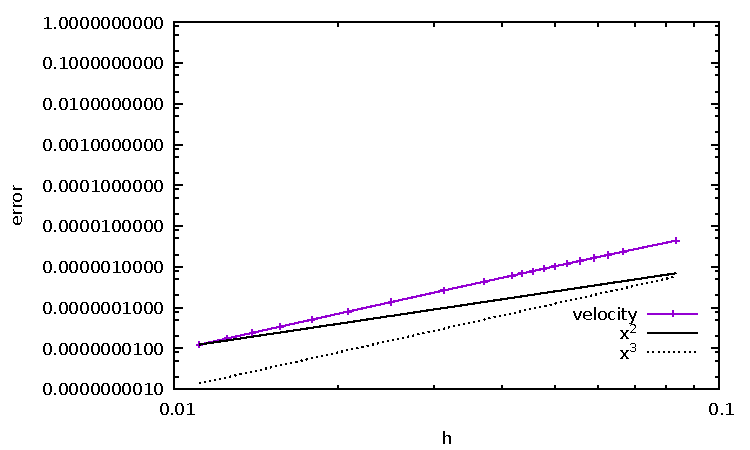
\includegraphics[width=10cm]{python_codes/fieldstone_19/errors}
\end{center}

velocity error rate is cubic, pressure superconvergent since the pressure field
is quadratic and therefore lies into the Q2 space.


\newpage
%%%%%%%%%%%%%%%%%%%%%%%%%%%%%%%%%%%%%%%%%%%%%%%%%%%%%%%%%%%%%%%%%%%%%%%%%%%%%%%
\section{{\tt fieldstone\_02}: Stokes sphere \label{f02}}
The details of the numerical setup are presented in Section \ref{f1}.

Each element has $m_V=16$ vertices so in total $ndof_V\times m_V=32$ 
velocity dofs and 
$ndof_P*m_P=9$ pressure dofs. The total number of 
velocity dofs is therefore $NfemV=nnp \times ndofV$ while the total number of
pressure dofs is $NfemP=nel$. The total number of dofs is then $Nfem=NfemV+NfemP$.

As a consequence, matrix $\K$ has size $NfemV,NfemV$ and matrix $\G$ has size $NfemV,NfemP$.
Vector $f$ is of size $NfemV$ and vector $h$ is of size $NfemP$.  

\begin{verbatim}

60===61===62===63===64===65===66===67===68===70
||             ||             ||             ||
50   51   52   53   54   55   56   57   58   59
||             ||             ||             ||
40   41   42   43   44   45   46   47   48   49
||             ||             ||             ||
30===31===32===33===34===35===36===37===38===39
||             ||             ||             ||
20   21   22   23   24   25   26   27   28   29
||             ||             ||             ||
10   11   12   13   14   15   16   17   18   19
||             ||             ||             ||
00===01===02===03===04===05===06===07===08===09

Example of 3x2 mesh. nnx=10, nny=7, nnp=70, nelx=3, nely=2, nel=6
\end{verbatim}


\begin{verbatim}
12===13===14===15           06=====07=====08
||   ||   ||   ||           ||     ||     ||
08===09===10===11           ||     ||     ||
||   ||   ||   ||           03=====04=====05
04===05===06===07           ||     ||     ||
||   ||   ||   ||           ||     ||     ||
00===01===02===03           00=====01=====02

Velocity (Q3)               Pressure (Q2)

(r,s)_{00}=(-1,-1)          (r,s)_{00}=(-1,-1) 
(r,s)_{01}=(-1/3,-1)        (r,s)_{01}=(0,-1) 
(r,s)_{02}=(+1/3,-1)        (r,s)_{02}=(+1,-1) 
(r,s)_{03}=(+1,-1)          (r,s)_{03}=(-1,0) 
(r,s)_{04}=(-1,-1/3)        (r,s)_{04}=(0,0) 
(r,s)_{05}=(-1/3,-1/3)      (r,s)_{05}=(+1,0) 
(r,s)_{06}=(+1/3,-1/3)      (r,s)_{06}=(-1,+1) 
(r,s)_{07}=(+1,-1/3)        (r,s)_{07}=(0,+1) 
(r,s)_{08}=(-1,+1/3)        (r,s)_{08}=(+1,+1) 
(r,s)_{09}=(-1/3,+1/3)
(r,s)_{10}=(+1/3,+1/3)
(r,s)_{11}=(+1,+1/3)
(r,s)_{12}=(-1,+1)
(r,s)_{13}=(-1/3,+1)
(r,s)_{14}=(+1/3,+1)
(r,s)_{15}=(+1,+1)

\end{verbatim}







{\color{red} Write about 4 point quadrature}.








\fbox{
\parbox{10cm}{{\bf features}
\begin{itemize}
\item $Q_3\times Q_2$ element \index{$Q_3 \times Q_2$}
\item incompressible flow \index{incompressible flow}
\item mixed formulation \index{mixed formulation}
\item isothermal \index{isothermal}
\item isoviscous \index{isoviscous}
\item analytical solution \index{analytical solution}
\end{itemize}
}}

\begin{center}
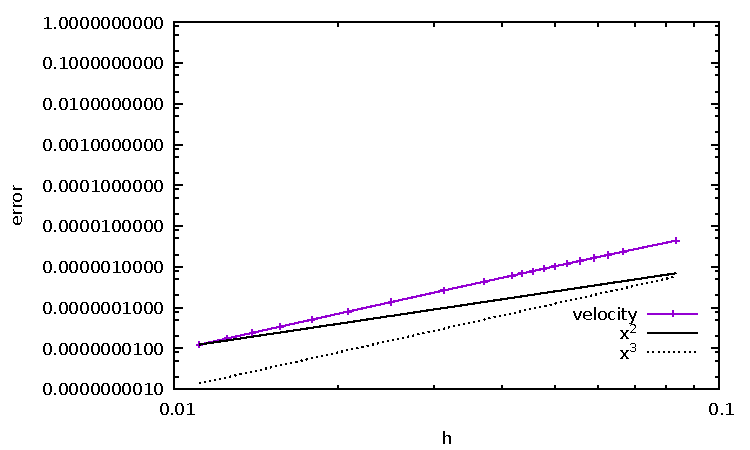
\includegraphics[width=10cm]{python_codes/fieldstone_19/errors}
\end{center}

velocity error rate is cubic, pressure superconvergent since the pressure field
is quadratic and therefore lies into the Q2 space.


\newpage
%%%%%%%%%%%%%%%%%%%%%%%%%%%%%%%%%%%%%%%%%%%%%%%%%%%%%%%%%%%%%%%%%%%%%%%%%%%%%%%
\section{{\tt fieldstone\_03}: Convection in a 2D box \label{f03}}
The details of the numerical setup are presented in Section \ref{f1}.

Each element has $m_V=16$ vertices so in total $ndof_V\times m_V=32$ 
velocity dofs and 
$ndof_P*m_P=9$ pressure dofs. The total number of 
velocity dofs is therefore $NfemV=nnp \times ndofV$ while the total number of
pressure dofs is $NfemP=nel$. The total number of dofs is then $Nfem=NfemV+NfemP$.

As a consequence, matrix $\K$ has size $NfemV,NfemV$ and matrix $\G$ has size $NfemV,NfemP$.
Vector $f$ is of size $NfemV$ and vector $h$ is of size $NfemP$.  

\begin{verbatim}

60===61===62===63===64===65===66===67===68===70
||             ||             ||             ||
50   51   52   53   54   55   56   57   58   59
||             ||             ||             ||
40   41   42   43   44   45   46   47   48   49
||             ||             ||             ||
30===31===32===33===34===35===36===37===38===39
||             ||             ||             ||
20   21   22   23   24   25   26   27   28   29
||             ||             ||             ||
10   11   12   13   14   15   16   17   18   19
||             ||             ||             ||
00===01===02===03===04===05===06===07===08===09

Example of 3x2 mesh. nnx=10, nny=7, nnp=70, nelx=3, nely=2, nel=6
\end{verbatim}


\begin{verbatim}
12===13===14===15           06=====07=====08
||   ||   ||   ||           ||     ||     ||
08===09===10===11           ||     ||     ||
||   ||   ||   ||           03=====04=====05
04===05===06===07           ||     ||     ||
||   ||   ||   ||           ||     ||     ||
00===01===02===03           00=====01=====02

Velocity (Q3)               Pressure (Q2)

(r,s)_{00}=(-1,-1)          (r,s)_{00}=(-1,-1) 
(r,s)_{01}=(-1/3,-1)        (r,s)_{01}=(0,-1) 
(r,s)_{02}=(+1/3,-1)        (r,s)_{02}=(+1,-1) 
(r,s)_{03}=(+1,-1)          (r,s)_{03}=(-1,0) 
(r,s)_{04}=(-1,-1/3)        (r,s)_{04}=(0,0) 
(r,s)_{05}=(-1/3,-1/3)      (r,s)_{05}=(+1,0) 
(r,s)_{06}=(+1/3,-1/3)      (r,s)_{06}=(-1,+1) 
(r,s)_{07}=(+1,-1/3)        (r,s)_{07}=(0,+1) 
(r,s)_{08}=(-1,+1/3)        (r,s)_{08}=(+1,+1) 
(r,s)_{09}=(-1/3,+1/3)
(r,s)_{10}=(+1/3,+1/3)
(r,s)_{11}=(+1,+1/3)
(r,s)_{12}=(-1,+1)
(r,s)_{13}=(-1/3,+1)
(r,s)_{14}=(+1/3,+1)
(r,s)_{15}=(+1,+1)

\end{verbatim}







{\color{red} Write about 4 point quadrature}.








\fbox{
\parbox{10cm}{{\bf features}
\begin{itemize}
\item $Q_3\times Q_2$ element \index{$Q_3 \times Q_2$}
\item incompressible flow \index{incompressible flow}
\item mixed formulation \index{mixed formulation}
\item isothermal \index{isothermal}
\item isoviscous \index{isoviscous}
\item analytical solution \index{analytical solution}
\end{itemize}
}}

\begin{center}
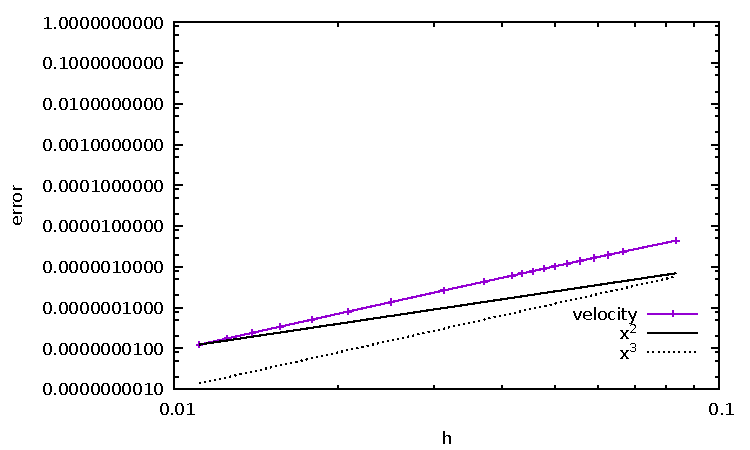
\includegraphics[width=10cm]{python_codes/fieldstone_19/errors}
\end{center}

velocity error rate is cubic, pressure superconvergent since the pressure field
is quadratic and therefore lies into the Q2 space.


\newpage
%%%%%%%%%%%%%%%%%%%%%%%%%%%%%%%%%%%%%%%%%%%%%%%%%%%%%%%%%%%%%%%%%%%%%%%%%%%%%%%
\section{{\tt fieldstone\_04}: The lid driven cavity \label{f04}}
The details of the numerical setup are presented in Section \ref{f1}.

Each element has $m_V=16$ vertices so in total $ndof_V\times m_V=32$ 
velocity dofs and 
$ndof_P*m_P=9$ pressure dofs. The total number of 
velocity dofs is therefore $NfemV=nnp \times ndofV$ while the total number of
pressure dofs is $NfemP=nel$. The total number of dofs is then $Nfem=NfemV+NfemP$.

As a consequence, matrix $\K$ has size $NfemV,NfemV$ and matrix $\G$ has size $NfemV,NfemP$.
Vector $f$ is of size $NfemV$ and vector $h$ is of size $NfemP$.  

\begin{verbatim}

60===61===62===63===64===65===66===67===68===70
||             ||             ||             ||
50   51   52   53   54   55   56   57   58   59
||             ||             ||             ||
40   41   42   43   44   45   46   47   48   49
||             ||             ||             ||
30===31===32===33===34===35===36===37===38===39
||             ||             ||             ||
20   21   22   23   24   25   26   27   28   29
||             ||             ||             ||
10   11   12   13   14   15   16   17   18   19
||             ||             ||             ||
00===01===02===03===04===05===06===07===08===09

Example of 3x2 mesh. nnx=10, nny=7, nnp=70, nelx=3, nely=2, nel=6
\end{verbatim}


\begin{verbatim}
12===13===14===15           06=====07=====08
||   ||   ||   ||           ||     ||     ||
08===09===10===11           ||     ||     ||
||   ||   ||   ||           03=====04=====05
04===05===06===07           ||     ||     ||
||   ||   ||   ||           ||     ||     ||
00===01===02===03           00=====01=====02

Velocity (Q3)               Pressure (Q2)

(r,s)_{00}=(-1,-1)          (r,s)_{00}=(-1,-1) 
(r,s)_{01}=(-1/3,-1)        (r,s)_{01}=(0,-1) 
(r,s)_{02}=(+1/3,-1)        (r,s)_{02}=(+1,-1) 
(r,s)_{03}=(+1,-1)          (r,s)_{03}=(-1,0) 
(r,s)_{04}=(-1,-1/3)        (r,s)_{04}=(0,0) 
(r,s)_{05}=(-1/3,-1/3)      (r,s)_{05}=(+1,0) 
(r,s)_{06}=(+1/3,-1/3)      (r,s)_{06}=(-1,+1) 
(r,s)_{07}=(+1,-1/3)        (r,s)_{07}=(0,+1) 
(r,s)_{08}=(-1,+1/3)        (r,s)_{08}=(+1,+1) 
(r,s)_{09}=(-1/3,+1/3)
(r,s)_{10}=(+1/3,+1/3)
(r,s)_{11}=(+1,+1/3)
(r,s)_{12}=(-1,+1)
(r,s)_{13}=(-1/3,+1)
(r,s)_{14}=(+1/3,+1)
(r,s)_{15}=(+1,+1)

\end{verbatim}







{\color{red} Write about 4 point quadrature}.








\fbox{
\parbox{10cm}{{\bf features}
\begin{itemize}
\item $Q_3\times Q_2$ element \index{$Q_3 \times Q_2$}
\item incompressible flow \index{incompressible flow}
\item mixed formulation \index{mixed formulation}
\item isothermal \index{isothermal}
\item isoviscous \index{isoviscous}
\item analytical solution \index{analytical solution}
\end{itemize}
}}

\begin{center}
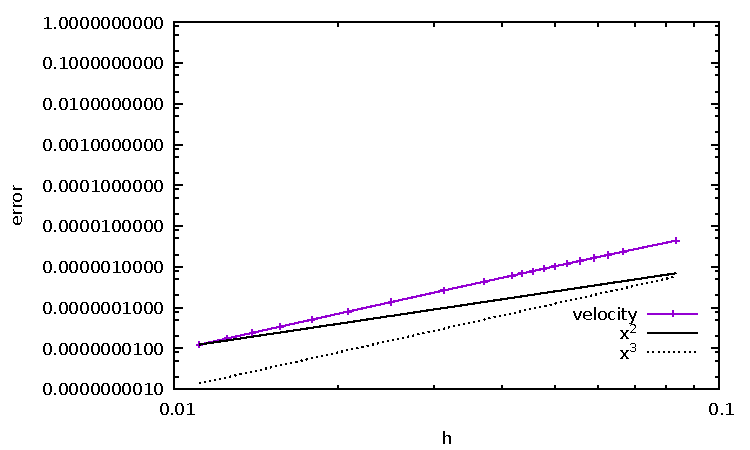
\includegraphics[width=10cm]{python_codes/fieldstone_19/errors}
\end{center}

velocity error rate is cubic, pressure superconvergent since the pressure field
is quadratic and therefore lies into the Q2 space.



\newpage
%%%%%%%%%%%%%%%%%%%%%%%%%%%%%%%%%%%%%%%%%%%%%%%%%%%%%%%%%%%%%%%%%%%%%%%%%%%%%%%
\section{{\tt fieldstone\_05}: SolCx benchmark \label{f05}}
The details of the numerical setup are presented in Section \ref{f1}.

Each element has $m_V=16$ vertices so in total $ndof_V\times m_V=32$ 
velocity dofs and 
$ndof_P*m_P=9$ pressure dofs. The total number of 
velocity dofs is therefore $NfemV=nnp \times ndofV$ while the total number of
pressure dofs is $NfemP=nel$. The total number of dofs is then $Nfem=NfemV+NfemP$.

As a consequence, matrix $\K$ has size $NfemV,NfemV$ and matrix $\G$ has size $NfemV,NfemP$.
Vector $f$ is of size $NfemV$ and vector $h$ is of size $NfemP$.  

\begin{verbatim}

60===61===62===63===64===65===66===67===68===70
||             ||             ||             ||
50   51   52   53   54   55   56   57   58   59
||             ||             ||             ||
40   41   42   43   44   45   46   47   48   49
||             ||             ||             ||
30===31===32===33===34===35===36===37===38===39
||             ||             ||             ||
20   21   22   23   24   25   26   27   28   29
||             ||             ||             ||
10   11   12   13   14   15   16   17   18   19
||             ||             ||             ||
00===01===02===03===04===05===06===07===08===09

Example of 3x2 mesh. nnx=10, nny=7, nnp=70, nelx=3, nely=2, nel=6
\end{verbatim}


\begin{verbatim}
12===13===14===15           06=====07=====08
||   ||   ||   ||           ||     ||     ||
08===09===10===11           ||     ||     ||
||   ||   ||   ||           03=====04=====05
04===05===06===07           ||     ||     ||
||   ||   ||   ||           ||     ||     ||
00===01===02===03           00=====01=====02

Velocity (Q3)               Pressure (Q2)

(r,s)_{00}=(-1,-1)          (r,s)_{00}=(-1,-1) 
(r,s)_{01}=(-1/3,-1)        (r,s)_{01}=(0,-1) 
(r,s)_{02}=(+1/3,-1)        (r,s)_{02}=(+1,-1) 
(r,s)_{03}=(+1,-1)          (r,s)_{03}=(-1,0) 
(r,s)_{04}=(-1,-1/3)        (r,s)_{04}=(0,0) 
(r,s)_{05}=(-1/3,-1/3)      (r,s)_{05}=(+1,0) 
(r,s)_{06}=(+1/3,-1/3)      (r,s)_{06}=(-1,+1) 
(r,s)_{07}=(+1,-1/3)        (r,s)_{07}=(0,+1) 
(r,s)_{08}=(-1,+1/3)        (r,s)_{08}=(+1,+1) 
(r,s)_{09}=(-1/3,+1/3)
(r,s)_{10}=(+1/3,+1/3)
(r,s)_{11}=(+1,+1/3)
(r,s)_{12}=(-1,+1)
(r,s)_{13}=(-1/3,+1)
(r,s)_{14}=(+1/3,+1)
(r,s)_{15}=(+1,+1)

\end{verbatim}







{\color{red} Write about 4 point quadrature}.








\fbox{
\parbox{10cm}{{\bf features}
\begin{itemize}
\item $Q_3\times Q_2$ element \index{$Q_3 \times Q_2$}
\item incompressible flow \index{incompressible flow}
\item mixed formulation \index{mixed formulation}
\item isothermal \index{isothermal}
\item isoviscous \index{isoviscous}
\item analytical solution \index{analytical solution}
\end{itemize}
}}

\begin{center}
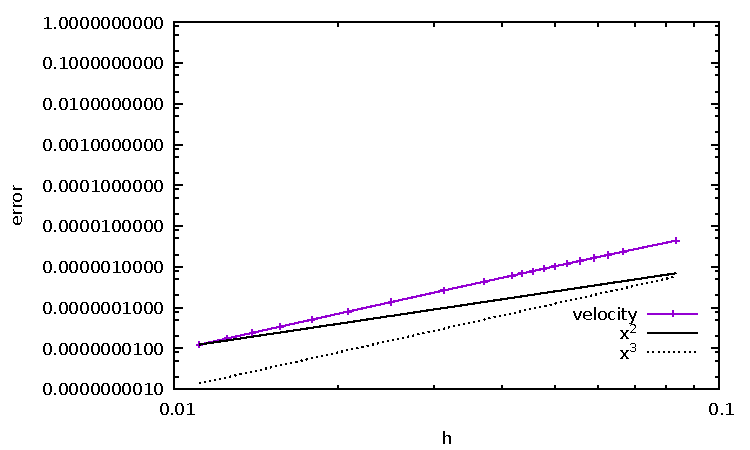
\includegraphics[width=10cm]{python_codes/fieldstone_19/errors}
\end{center}

velocity error rate is cubic, pressure superconvergent since the pressure field
is quadratic and therefore lies into the Q2 space.


\newpage
%%%%%%%%%%%%%%%%%%%%%%%%%%%%%%%%%%%%%%%%%%%%%%%%%%%%%%%%%%%%%%%%%%%%%%%%%%%%%%%
\section{{\tt fieldstone\_06}: SolKz benchmark \label{f06}}
The details of the numerical setup are presented in Section \ref{f1}.

Each element has $m_V=16$ vertices so in total $ndof_V\times m_V=32$ 
velocity dofs and 
$ndof_P*m_P=9$ pressure dofs. The total number of 
velocity dofs is therefore $NfemV=nnp \times ndofV$ while the total number of
pressure dofs is $NfemP=nel$. The total number of dofs is then $Nfem=NfemV+NfemP$.

As a consequence, matrix $\K$ has size $NfemV,NfemV$ and matrix $\G$ has size $NfemV,NfemP$.
Vector $f$ is of size $NfemV$ and vector $h$ is of size $NfemP$.  

\begin{verbatim}

60===61===62===63===64===65===66===67===68===70
||             ||             ||             ||
50   51   52   53   54   55   56   57   58   59
||             ||             ||             ||
40   41   42   43   44   45   46   47   48   49
||             ||             ||             ||
30===31===32===33===34===35===36===37===38===39
||             ||             ||             ||
20   21   22   23   24   25   26   27   28   29
||             ||             ||             ||
10   11   12   13   14   15   16   17   18   19
||             ||             ||             ||
00===01===02===03===04===05===06===07===08===09

Example of 3x2 mesh. nnx=10, nny=7, nnp=70, nelx=3, nely=2, nel=6
\end{verbatim}


\begin{verbatim}
12===13===14===15           06=====07=====08
||   ||   ||   ||           ||     ||     ||
08===09===10===11           ||     ||     ||
||   ||   ||   ||           03=====04=====05
04===05===06===07           ||     ||     ||
||   ||   ||   ||           ||     ||     ||
00===01===02===03           00=====01=====02

Velocity (Q3)               Pressure (Q2)

(r,s)_{00}=(-1,-1)          (r,s)_{00}=(-1,-1) 
(r,s)_{01}=(-1/3,-1)        (r,s)_{01}=(0,-1) 
(r,s)_{02}=(+1/3,-1)        (r,s)_{02}=(+1,-1) 
(r,s)_{03}=(+1,-1)          (r,s)_{03}=(-1,0) 
(r,s)_{04}=(-1,-1/3)        (r,s)_{04}=(0,0) 
(r,s)_{05}=(-1/3,-1/3)      (r,s)_{05}=(+1,0) 
(r,s)_{06}=(+1/3,-1/3)      (r,s)_{06}=(-1,+1) 
(r,s)_{07}=(+1,-1/3)        (r,s)_{07}=(0,+1) 
(r,s)_{08}=(-1,+1/3)        (r,s)_{08}=(+1,+1) 
(r,s)_{09}=(-1/3,+1/3)
(r,s)_{10}=(+1/3,+1/3)
(r,s)_{11}=(+1,+1/3)
(r,s)_{12}=(-1,+1)
(r,s)_{13}=(-1/3,+1)
(r,s)_{14}=(+1/3,+1)
(r,s)_{15}=(+1,+1)

\end{verbatim}







{\color{red} Write about 4 point quadrature}.








\fbox{
\parbox{10cm}{{\bf features}
\begin{itemize}
\item $Q_3\times Q_2$ element \index{$Q_3 \times Q_2$}
\item incompressible flow \index{incompressible flow}
\item mixed formulation \index{mixed formulation}
\item isothermal \index{isothermal}
\item isoviscous \index{isoviscous}
\item analytical solution \index{analytical solution}
\end{itemize}
}}

\begin{center}
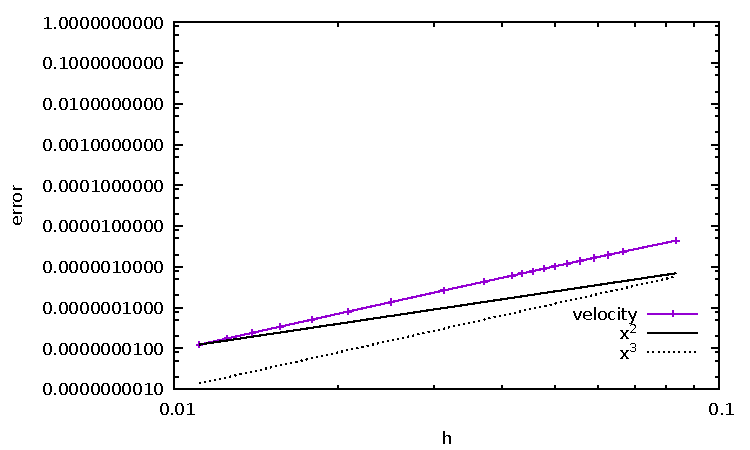
\includegraphics[width=10cm]{python_codes/fieldstone_19/errors}
\end{center}

velocity error rate is cubic, pressure superconvergent since the pressure field
is quadratic and therefore lies into the Q2 space.


\newpage
%%%%%%%%%%%%%%%%%%%%%%%%%%%%%%%%%%%%%%%%%%%%%%%%%%%%%%%%%%%%%%%%%%%%%%%%%%%%%%%
\section{{\tt fieldstone\_07}: SolVi benchmark \label{f07}}
The details of the numerical setup are presented in Section \ref{f1}.

Each element has $m_V=16$ vertices so in total $ndof_V\times m_V=32$ 
velocity dofs and 
$ndof_P*m_P=9$ pressure dofs. The total number of 
velocity dofs is therefore $NfemV=nnp \times ndofV$ while the total number of
pressure dofs is $NfemP=nel$. The total number of dofs is then $Nfem=NfemV+NfemP$.

As a consequence, matrix $\K$ has size $NfemV,NfemV$ and matrix $\G$ has size $NfemV,NfemP$.
Vector $f$ is of size $NfemV$ and vector $h$ is of size $NfemP$.  

\begin{verbatim}

60===61===62===63===64===65===66===67===68===70
||             ||             ||             ||
50   51   52   53   54   55   56   57   58   59
||             ||             ||             ||
40   41   42   43   44   45   46   47   48   49
||             ||             ||             ||
30===31===32===33===34===35===36===37===38===39
||             ||             ||             ||
20   21   22   23   24   25   26   27   28   29
||             ||             ||             ||
10   11   12   13   14   15   16   17   18   19
||             ||             ||             ||
00===01===02===03===04===05===06===07===08===09

Example of 3x2 mesh. nnx=10, nny=7, nnp=70, nelx=3, nely=2, nel=6
\end{verbatim}


\begin{verbatim}
12===13===14===15           06=====07=====08
||   ||   ||   ||           ||     ||     ||
08===09===10===11           ||     ||     ||
||   ||   ||   ||           03=====04=====05
04===05===06===07           ||     ||     ||
||   ||   ||   ||           ||     ||     ||
00===01===02===03           00=====01=====02

Velocity (Q3)               Pressure (Q2)

(r,s)_{00}=(-1,-1)          (r,s)_{00}=(-1,-1) 
(r,s)_{01}=(-1/3,-1)        (r,s)_{01}=(0,-1) 
(r,s)_{02}=(+1/3,-1)        (r,s)_{02}=(+1,-1) 
(r,s)_{03}=(+1,-1)          (r,s)_{03}=(-1,0) 
(r,s)_{04}=(-1,-1/3)        (r,s)_{04}=(0,0) 
(r,s)_{05}=(-1/3,-1/3)      (r,s)_{05}=(+1,0) 
(r,s)_{06}=(+1/3,-1/3)      (r,s)_{06}=(-1,+1) 
(r,s)_{07}=(+1,-1/3)        (r,s)_{07}=(0,+1) 
(r,s)_{08}=(-1,+1/3)        (r,s)_{08}=(+1,+1) 
(r,s)_{09}=(-1/3,+1/3)
(r,s)_{10}=(+1/3,+1/3)
(r,s)_{11}=(+1,+1/3)
(r,s)_{12}=(-1,+1)
(r,s)_{13}=(-1/3,+1)
(r,s)_{14}=(+1/3,+1)
(r,s)_{15}=(+1,+1)

\end{verbatim}







{\color{red} Write about 4 point quadrature}.








\fbox{
\parbox{10cm}{{\bf features}
\begin{itemize}
\item $Q_3\times Q_2$ element \index{$Q_3 \times Q_2$}
\item incompressible flow \index{incompressible flow}
\item mixed formulation \index{mixed formulation}
\item isothermal \index{isothermal}
\item isoviscous \index{isoviscous}
\item analytical solution \index{analytical solution}
\end{itemize}
}}

\begin{center}
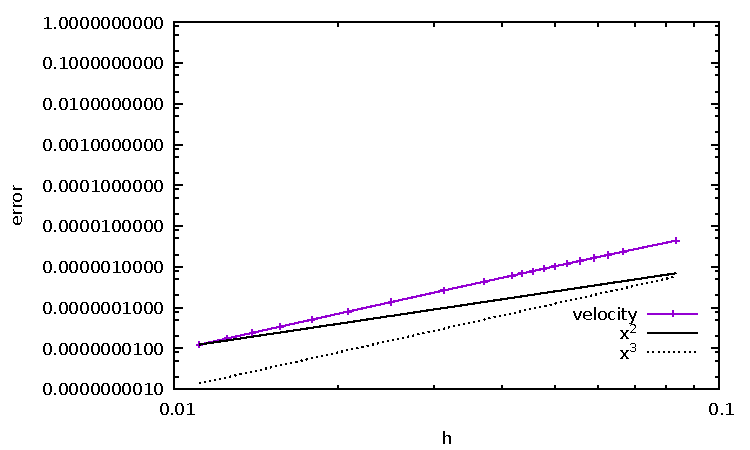
\includegraphics[width=10cm]{python_codes/fieldstone_19/errors}
\end{center}

velocity error rate is cubic, pressure superconvergent since the pressure field
is quadratic and therefore lies into the Q2 space.


\newpage
%%%%%%%%%%%%%%%%%%%%%%%%%%%%%%%%%%%%%%%%%%%%%%%%%%%%%%%%%%%%%%%%%%%%%%%%%%%%%%%
\section{{\tt fieldstone\_08}: the indentor benchmark \label{f08}}
The details of the numerical setup are presented in Section \ref{f1}.

Each element has $m_V=16$ vertices so in total $ndof_V\times m_V=32$ 
velocity dofs and 
$ndof_P*m_P=9$ pressure dofs. The total number of 
velocity dofs is therefore $NfemV=nnp \times ndofV$ while the total number of
pressure dofs is $NfemP=nel$. The total number of dofs is then $Nfem=NfemV+NfemP$.

As a consequence, matrix $\K$ has size $NfemV,NfemV$ and matrix $\G$ has size $NfemV,NfemP$.
Vector $f$ is of size $NfemV$ and vector $h$ is of size $NfemP$.  

\begin{verbatim}

60===61===62===63===64===65===66===67===68===70
||             ||             ||             ||
50   51   52   53   54   55   56   57   58   59
||             ||             ||             ||
40   41   42   43   44   45   46   47   48   49
||             ||             ||             ||
30===31===32===33===34===35===36===37===38===39
||             ||             ||             ||
20   21   22   23   24   25   26   27   28   29
||             ||             ||             ||
10   11   12   13   14   15   16   17   18   19
||             ||             ||             ||
00===01===02===03===04===05===06===07===08===09

Example of 3x2 mesh. nnx=10, nny=7, nnp=70, nelx=3, nely=2, nel=6
\end{verbatim}


\begin{verbatim}
12===13===14===15           06=====07=====08
||   ||   ||   ||           ||     ||     ||
08===09===10===11           ||     ||     ||
||   ||   ||   ||           03=====04=====05
04===05===06===07           ||     ||     ||
||   ||   ||   ||           ||     ||     ||
00===01===02===03           00=====01=====02

Velocity (Q3)               Pressure (Q2)

(r,s)_{00}=(-1,-1)          (r,s)_{00}=(-1,-1) 
(r,s)_{01}=(-1/3,-1)        (r,s)_{01}=(0,-1) 
(r,s)_{02}=(+1/3,-1)        (r,s)_{02}=(+1,-1) 
(r,s)_{03}=(+1,-1)          (r,s)_{03}=(-1,0) 
(r,s)_{04}=(-1,-1/3)        (r,s)_{04}=(0,0) 
(r,s)_{05}=(-1/3,-1/3)      (r,s)_{05}=(+1,0) 
(r,s)_{06}=(+1/3,-1/3)      (r,s)_{06}=(-1,+1) 
(r,s)_{07}=(+1,-1/3)        (r,s)_{07}=(0,+1) 
(r,s)_{08}=(-1,+1/3)        (r,s)_{08}=(+1,+1) 
(r,s)_{09}=(-1/3,+1/3)
(r,s)_{10}=(+1/3,+1/3)
(r,s)_{11}=(+1,+1/3)
(r,s)_{12}=(-1,+1)
(r,s)_{13}=(-1/3,+1)
(r,s)_{14}=(+1/3,+1)
(r,s)_{15}=(+1,+1)

\end{verbatim}







{\color{red} Write about 4 point quadrature}.








\fbox{
\parbox{10cm}{{\bf features}
\begin{itemize}
\item $Q_3\times Q_2$ element \index{$Q_3 \times Q_2$}
\item incompressible flow \index{incompressible flow}
\item mixed formulation \index{mixed formulation}
\item isothermal \index{isothermal}
\item isoviscous \index{isoviscous}
\item analytical solution \index{analytical solution}
\end{itemize}
}}

\begin{center}
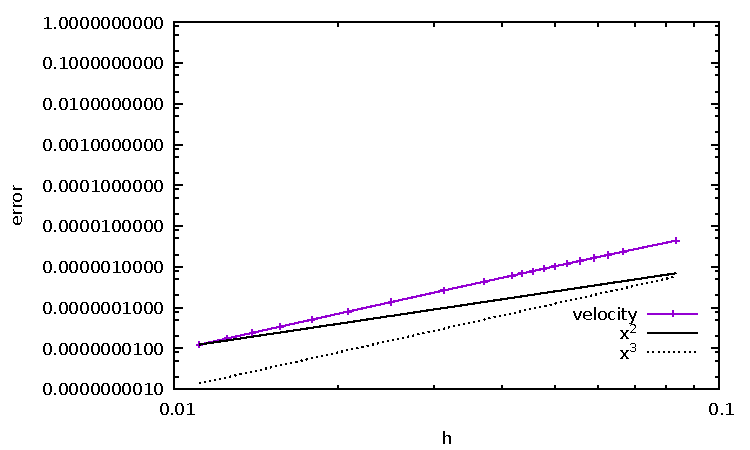
\includegraphics[width=10cm]{python_codes/fieldstone_19/errors}
\end{center}

velocity error rate is cubic, pressure superconvergent since the pressure field
is quadratic and therefore lies into the Q2 space.


\newpage
%%%%%%%%%%%%%%%%%%%%%%%%%%%%%%%%%%%%%%%%%%%%%%%%%%%%%%%%%%%%%%%%%%%%%%%%%%%%%%%
\section{{\tt fieldstone\_09}: the annulus benchmark \label{f09}}
The details of the numerical setup are presented in Section \ref{f1}.

Each element has $m_V=16$ vertices so in total $ndof_V\times m_V=32$ 
velocity dofs and 
$ndof_P*m_P=9$ pressure dofs. The total number of 
velocity dofs is therefore $NfemV=nnp \times ndofV$ while the total number of
pressure dofs is $NfemP=nel$. The total number of dofs is then $Nfem=NfemV+NfemP$.

As a consequence, matrix $\K$ has size $NfemV,NfemV$ and matrix $\G$ has size $NfemV,NfemP$.
Vector $f$ is of size $NfemV$ and vector $h$ is of size $NfemP$.  

\begin{verbatim}

60===61===62===63===64===65===66===67===68===70
||             ||             ||             ||
50   51   52   53   54   55   56   57   58   59
||             ||             ||             ||
40   41   42   43   44   45   46   47   48   49
||             ||             ||             ||
30===31===32===33===34===35===36===37===38===39
||             ||             ||             ||
20   21   22   23   24   25   26   27   28   29
||             ||             ||             ||
10   11   12   13   14   15   16   17   18   19
||             ||             ||             ||
00===01===02===03===04===05===06===07===08===09

Example of 3x2 mesh. nnx=10, nny=7, nnp=70, nelx=3, nely=2, nel=6
\end{verbatim}


\begin{verbatim}
12===13===14===15           06=====07=====08
||   ||   ||   ||           ||     ||     ||
08===09===10===11           ||     ||     ||
||   ||   ||   ||           03=====04=====05
04===05===06===07           ||     ||     ||
||   ||   ||   ||           ||     ||     ||
00===01===02===03           00=====01=====02

Velocity (Q3)               Pressure (Q2)

(r,s)_{00}=(-1,-1)          (r,s)_{00}=(-1,-1) 
(r,s)_{01}=(-1/3,-1)        (r,s)_{01}=(0,-1) 
(r,s)_{02}=(+1/3,-1)        (r,s)_{02}=(+1,-1) 
(r,s)_{03}=(+1,-1)          (r,s)_{03}=(-1,0) 
(r,s)_{04}=(-1,-1/3)        (r,s)_{04}=(0,0) 
(r,s)_{05}=(-1/3,-1/3)      (r,s)_{05}=(+1,0) 
(r,s)_{06}=(+1/3,-1/3)      (r,s)_{06}=(-1,+1) 
(r,s)_{07}=(+1,-1/3)        (r,s)_{07}=(0,+1) 
(r,s)_{08}=(-1,+1/3)        (r,s)_{08}=(+1,+1) 
(r,s)_{09}=(-1/3,+1/3)
(r,s)_{10}=(+1/3,+1/3)
(r,s)_{11}=(+1,+1/3)
(r,s)_{12}=(-1,+1)
(r,s)_{13}=(-1/3,+1)
(r,s)_{14}=(+1/3,+1)
(r,s)_{15}=(+1,+1)

\end{verbatim}







{\color{red} Write about 4 point quadrature}.








\fbox{
\parbox{10cm}{{\bf features}
\begin{itemize}
\item $Q_3\times Q_2$ element \index{$Q_3 \times Q_2$}
\item incompressible flow \index{incompressible flow}
\item mixed formulation \index{mixed formulation}
\item isothermal \index{isothermal}
\item isoviscous \index{isoviscous}
\item analytical solution \index{analytical solution}
\end{itemize}
}}

\begin{center}
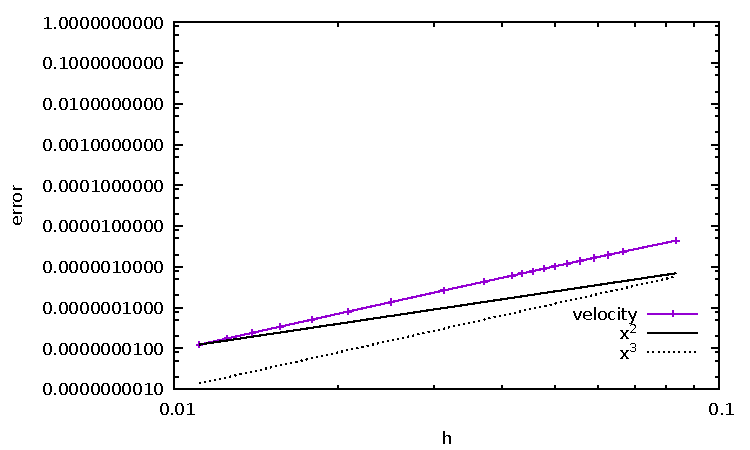
\includegraphics[width=10cm]{python_codes/fieldstone_19/errors}
\end{center}

velocity error rate is cubic, pressure superconvergent since the pressure field
is quadratic and therefore lies into the Q2 space.



\newpage
%%%%%%%%%%%%%%%%%%%%%%%%%%%%%%%%%%%%%%%%%%%%%%%%%%%%%%%%%%%%%%%%%%%%%%%%%%%%%%%
\section{{\tt fieldstone\_10}: Stokes sphere (3D) - penalty \label{f10}}
The details of the numerical setup are presented in Section \ref{f1}.

Each element has $m_V=16$ vertices so in total $ndof_V\times m_V=32$ 
velocity dofs and 
$ndof_P*m_P=9$ pressure dofs. The total number of 
velocity dofs is therefore $NfemV=nnp \times ndofV$ while the total number of
pressure dofs is $NfemP=nel$. The total number of dofs is then $Nfem=NfemV+NfemP$.

As a consequence, matrix $\K$ has size $NfemV,NfemV$ and matrix $\G$ has size $NfemV,NfemP$.
Vector $f$ is of size $NfemV$ and vector $h$ is of size $NfemP$.  

\begin{verbatim}

60===61===62===63===64===65===66===67===68===70
||             ||             ||             ||
50   51   52   53   54   55   56   57   58   59
||             ||             ||             ||
40   41   42   43   44   45   46   47   48   49
||             ||             ||             ||
30===31===32===33===34===35===36===37===38===39
||             ||             ||             ||
20   21   22   23   24   25   26   27   28   29
||             ||             ||             ||
10   11   12   13   14   15   16   17   18   19
||             ||             ||             ||
00===01===02===03===04===05===06===07===08===09

Example of 3x2 mesh. nnx=10, nny=7, nnp=70, nelx=3, nely=2, nel=6
\end{verbatim}


\begin{verbatim}
12===13===14===15           06=====07=====08
||   ||   ||   ||           ||     ||     ||
08===09===10===11           ||     ||     ||
||   ||   ||   ||           03=====04=====05
04===05===06===07           ||     ||     ||
||   ||   ||   ||           ||     ||     ||
00===01===02===03           00=====01=====02

Velocity (Q3)               Pressure (Q2)

(r,s)_{00}=(-1,-1)          (r,s)_{00}=(-1,-1) 
(r,s)_{01}=(-1/3,-1)        (r,s)_{01}=(0,-1) 
(r,s)_{02}=(+1/3,-1)        (r,s)_{02}=(+1,-1) 
(r,s)_{03}=(+1,-1)          (r,s)_{03}=(-1,0) 
(r,s)_{04}=(-1,-1/3)        (r,s)_{04}=(0,0) 
(r,s)_{05}=(-1/3,-1/3)      (r,s)_{05}=(+1,0) 
(r,s)_{06}=(+1/3,-1/3)      (r,s)_{06}=(-1,+1) 
(r,s)_{07}=(+1,-1/3)        (r,s)_{07}=(0,+1) 
(r,s)_{08}=(-1,+1/3)        (r,s)_{08}=(+1,+1) 
(r,s)_{09}=(-1/3,+1/3)
(r,s)_{10}=(+1/3,+1/3)
(r,s)_{11}=(+1,+1/3)
(r,s)_{12}=(-1,+1)
(r,s)_{13}=(-1/3,+1)
(r,s)_{14}=(+1/3,+1)
(r,s)_{15}=(+1,+1)

\end{verbatim}







{\color{red} Write about 4 point quadrature}.








\fbox{
\parbox{10cm}{{\bf features}
\begin{itemize}
\item $Q_3\times Q_2$ element \index{$Q_3 \times Q_2$}
\item incompressible flow \index{incompressible flow}
\item mixed formulation \index{mixed formulation}
\item isothermal \index{isothermal}
\item isoviscous \index{isoviscous}
\item analytical solution \index{analytical solution}
\end{itemize}
}}

\begin{center}
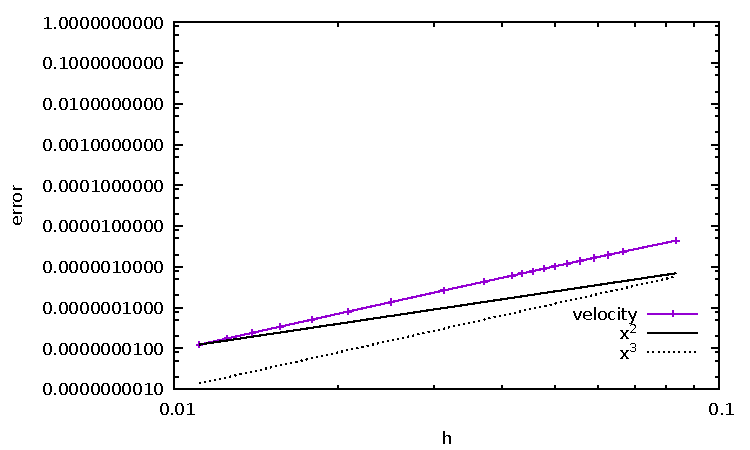
\includegraphics[width=10cm]{python_codes/fieldstone_19/errors}
\end{center}

velocity error rate is cubic, pressure superconvergent since the pressure field
is quadratic and therefore lies into the Q2 space.


\newpage
%%%%%%%%%%%%%%%%%%%%%%%%%%%%%%%%%%%%%%%%%%%%%%%%%%%%%%%%%%%%%%%%%%%%%%%%%%%%%%%
\section{{\tt fieldstone\_11}: stokes sphere (3D) - mixed formulation \label{f11}}
The details of the numerical setup are presented in Section \ref{f1}.

Each element has $m_V=16$ vertices so in total $ndof_V\times m_V=32$ 
velocity dofs and 
$ndof_P*m_P=9$ pressure dofs. The total number of 
velocity dofs is therefore $NfemV=nnp \times ndofV$ while the total number of
pressure dofs is $NfemP=nel$. The total number of dofs is then $Nfem=NfemV+NfemP$.

As a consequence, matrix $\K$ has size $NfemV,NfemV$ and matrix $\G$ has size $NfemV,NfemP$.
Vector $f$ is of size $NfemV$ and vector $h$ is of size $NfemP$.  

\begin{verbatim}

60===61===62===63===64===65===66===67===68===70
||             ||             ||             ||
50   51   52   53   54   55   56   57   58   59
||             ||             ||             ||
40   41   42   43   44   45   46   47   48   49
||             ||             ||             ||
30===31===32===33===34===35===36===37===38===39
||             ||             ||             ||
20   21   22   23   24   25   26   27   28   29
||             ||             ||             ||
10   11   12   13   14   15   16   17   18   19
||             ||             ||             ||
00===01===02===03===04===05===06===07===08===09

Example of 3x2 mesh. nnx=10, nny=7, nnp=70, nelx=3, nely=2, nel=6
\end{verbatim}


\begin{verbatim}
12===13===14===15           06=====07=====08
||   ||   ||   ||           ||     ||     ||
08===09===10===11           ||     ||     ||
||   ||   ||   ||           03=====04=====05
04===05===06===07           ||     ||     ||
||   ||   ||   ||           ||     ||     ||
00===01===02===03           00=====01=====02

Velocity (Q3)               Pressure (Q2)

(r,s)_{00}=(-1,-1)          (r,s)_{00}=(-1,-1) 
(r,s)_{01}=(-1/3,-1)        (r,s)_{01}=(0,-1) 
(r,s)_{02}=(+1/3,-1)        (r,s)_{02}=(+1,-1) 
(r,s)_{03}=(+1,-1)          (r,s)_{03}=(-1,0) 
(r,s)_{04}=(-1,-1/3)        (r,s)_{04}=(0,0) 
(r,s)_{05}=(-1/3,-1/3)      (r,s)_{05}=(+1,0) 
(r,s)_{06}=(+1/3,-1/3)      (r,s)_{06}=(-1,+1) 
(r,s)_{07}=(+1,-1/3)        (r,s)_{07}=(0,+1) 
(r,s)_{08}=(-1,+1/3)        (r,s)_{08}=(+1,+1) 
(r,s)_{09}=(-1/3,+1/3)
(r,s)_{10}=(+1/3,+1/3)
(r,s)_{11}=(+1,+1/3)
(r,s)_{12}=(-1,+1)
(r,s)_{13}=(-1/3,+1)
(r,s)_{14}=(+1/3,+1)
(r,s)_{15}=(+1,+1)

\end{verbatim}







{\color{red} Write about 4 point quadrature}.








\fbox{
\parbox{10cm}{{\bf features}
\begin{itemize}
\item $Q_3\times Q_2$ element \index{$Q_3 \times Q_2$}
\item incompressible flow \index{incompressible flow}
\item mixed formulation \index{mixed formulation}
\item isothermal \index{isothermal}
\item isoviscous \index{isoviscous}
\item analytical solution \index{analytical solution}
\end{itemize}
}}

\begin{center}
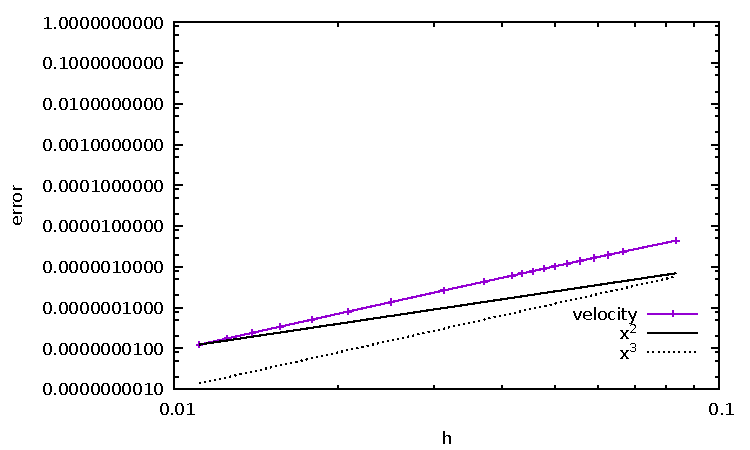
\includegraphics[width=10cm]{python_codes/fieldstone_19/errors}
\end{center}

velocity error rate is cubic, pressure superconvergent since the pressure field
is quadratic and therefore lies into the Q2 space.


\newpage
%%%%%%%%%%%%%%%%%%%%%%%%%%%%%%%%%%%%%%%%%%%%%%%%%%%%%%%%%%%%%%%%%%%%%%%%%%%%%%%
\section{{\tt fieldstone\_12}: consistent pressure recovery \label{f12}}
The details of the numerical setup are presented in Section \ref{f1}.

Each element has $m_V=16$ vertices so in total $ndof_V\times m_V=32$ 
velocity dofs and 
$ndof_P*m_P=9$ pressure dofs. The total number of 
velocity dofs is therefore $NfemV=nnp \times ndofV$ while the total number of
pressure dofs is $NfemP=nel$. The total number of dofs is then $Nfem=NfemV+NfemP$.

As a consequence, matrix $\K$ has size $NfemV,NfemV$ and matrix $\G$ has size $NfemV,NfemP$.
Vector $f$ is of size $NfemV$ and vector $h$ is of size $NfemP$.  

\begin{verbatim}

60===61===62===63===64===65===66===67===68===70
||             ||             ||             ||
50   51   52   53   54   55   56   57   58   59
||             ||             ||             ||
40   41   42   43   44   45   46   47   48   49
||             ||             ||             ||
30===31===32===33===34===35===36===37===38===39
||             ||             ||             ||
20   21   22   23   24   25   26   27   28   29
||             ||             ||             ||
10   11   12   13   14   15   16   17   18   19
||             ||             ||             ||
00===01===02===03===04===05===06===07===08===09

Example of 3x2 mesh. nnx=10, nny=7, nnp=70, nelx=3, nely=2, nel=6
\end{verbatim}


\begin{verbatim}
12===13===14===15           06=====07=====08
||   ||   ||   ||           ||     ||     ||
08===09===10===11           ||     ||     ||
||   ||   ||   ||           03=====04=====05
04===05===06===07           ||     ||     ||
||   ||   ||   ||           ||     ||     ||
00===01===02===03           00=====01=====02

Velocity (Q3)               Pressure (Q2)

(r,s)_{00}=(-1,-1)          (r,s)_{00}=(-1,-1) 
(r,s)_{01}=(-1/3,-1)        (r,s)_{01}=(0,-1) 
(r,s)_{02}=(+1/3,-1)        (r,s)_{02}=(+1,-1) 
(r,s)_{03}=(+1,-1)          (r,s)_{03}=(-1,0) 
(r,s)_{04}=(-1,-1/3)        (r,s)_{04}=(0,0) 
(r,s)_{05}=(-1/3,-1/3)      (r,s)_{05}=(+1,0) 
(r,s)_{06}=(+1/3,-1/3)      (r,s)_{06}=(-1,+1) 
(r,s)_{07}=(+1,-1/3)        (r,s)_{07}=(0,+1) 
(r,s)_{08}=(-1,+1/3)        (r,s)_{08}=(+1,+1) 
(r,s)_{09}=(-1/3,+1/3)
(r,s)_{10}=(+1/3,+1/3)
(r,s)_{11}=(+1,+1/3)
(r,s)_{12}=(-1,+1)
(r,s)_{13}=(-1/3,+1)
(r,s)_{14}=(+1/3,+1)
(r,s)_{15}=(+1,+1)

\end{verbatim}







{\color{red} Write about 4 point quadrature}.








\fbox{
\parbox{10cm}{{\bf features}
\begin{itemize}
\item $Q_3\times Q_2$ element \index{$Q_3 \times Q_2$}
\item incompressible flow \index{incompressible flow}
\item mixed formulation \index{mixed formulation}
\item isothermal \index{isothermal}
\item isoviscous \index{isoviscous}
\item analytical solution \index{analytical solution}
\end{itemize}
}}

\begin{center}
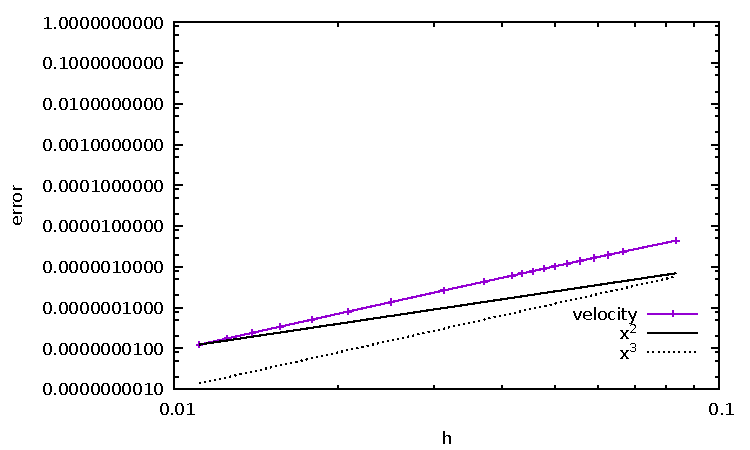
\includegraphics[width=10cm]{python_codes/fieldstone_19/errors}
\end{center}

velocity error rate is cubic, pressure superconvergent since the pressure field
is quadratic and therefore lies into the Q2 space.


\newpage
%%%%%%%%%%%%%%%%%%%%%%%%%%%%%%%%%%%%%%%%%%%%%%%%%%%%%%%%%%%%%%%%%%%%%%%%%%%%%%%
\section{{\tt fieldstone\_13}: the Particle in Cell technique (1) - the effect of averaging \label{f13}}
The details of the numerical setup are presented in Section \ref{f1}.

Each element has $m_V=16$ vertices so in total $ndof_V\times m_V=32$ 
velocity dofs and 
$ndof_P*m_P=9$ pressure dofs. The total number of 
velocity dofs is therefore $NfemV=nnp \times ndofV$ while the total number of
pressure dofs is $NfemP=nel$. The total number of dofs is then $Nfem=NfemV+NfemP$.

As a consequence, matrix $\K$ has size $NfemV,NfemV$ and matrix $\G$ has size $NfemV,NfemP$.
Vector $f$ is of size $NfemV$ and vector $h$ is of size $NfemP$.  

\begin{verbatim}

60===61===62===63===64===65===66===67===68===70
||             ||             ||             ||
50   51   52   53   54   55   56   57   58   59
||             ||             ||             ||
40   41   42   43   44   45   46   47   48   49
||             ||             ||             ||
30===31===32===33===34===35===36===37===38===39
||             ||             ||             ||
20   21   22   23   24   25   26   27   28   29
||             ||             ||             ||
10   11   12   13   14   15   16   17   18   19
||             ||             ||             ||
00===01===02===03===04===05===06===07===08===09

Example of 3x2 mesh. nnx=10, nny=7, nnp=70, nelx=3, nely=2, nel=6
\end{verbatim}


\begin{verbatim}
12===13===14===15           06=====07=====08
||   ||   ||   ||           ||     ||     ||
08===09===10===11           ||     ||     ||
||   ||   ||   ||           03=====04=====05
04===05===06===07           ||     ||     ||
||   ||   ||   ||           ||     ||     ||
00===01===02===03           00=====01=====02

Velocity (Q3)               Pressure (Q2)

(r,s)_{00}=(-1,-1)          (r,s)_{00}=(-1,-1) 
(r,s)_{01}=(-1/3,-1)        (r,s)_{01}=(0,-1) 
(r,s)_{02}=(+1/3,-1)        (r,s)_{02}=(+1,-1) 
(r,s)_{03}=(+1,-1)          (r,s)_{03}=(-1,0) 
(r,s)_{04}=(-1,-1/3)        (r,s)_{04}=(0,0) 
(r,s)_{05}=(-1/3,-1/3)      (r,s)_{05}=(+1,0) 
(r,s)_{06}=(+1/3,-1/3)      (r,s)_{06}=(-1,+1) 
(r,s)_{07}=(+1,-1/3)        (r,s)_{07}=(0,+1) 
(r,s)_{08}=(-1,+1/3)        (r,s)_{08}=(+1,+1) 
(r,s)_{09}=(-1/3,+1/3)
(r,s)_{10}=(+1/3,+1/3)
(r,s)_{11}=(+1,+1/3)
(r,s)_{12}=(-1,+1)
(r,s)_{13}=(-1/3,+1)
(r,s)_{14}=(+1/3,+1)
(r,s)_{15}=(+1,+1)

\end{verbatim}







{\color{red} Write about 4 point quadrature}.








\fbox{
\parbox{10cm}{{\bf features}
\begin{itemize}
\item $Q_3\times Q_2$ element \index{$Q_3 \times Q_2$}
\item incompressible flow \index{incompressible flow}
\item mixed formulation \index{mixed formulation}
\item isothermal \index{isothermal}
\item isoviscous \index{isoviscous}
\item analytical solution \index{analytical solution}
\end{itemize}
}}

\begin{center}
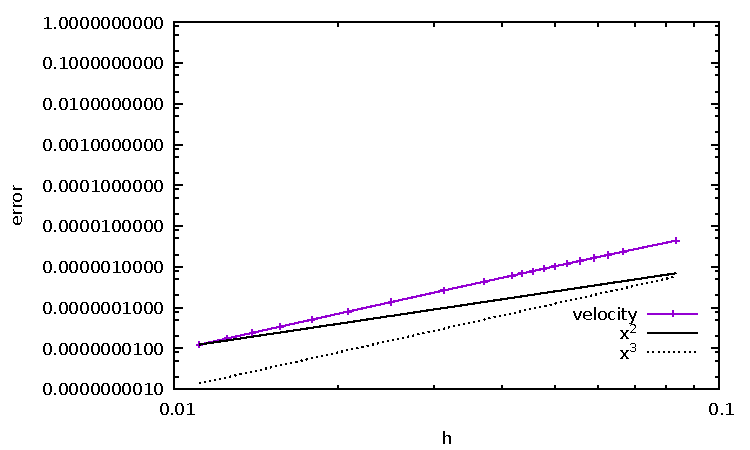
\includegraphics[width=10cm]{python_codes/fieldstone_19/errors}
\end{center}

velocity error rate is cubic, pressure superconvergent since the pressure field
is quadratic and therefore lies into the Q2 space.


\newpage
%%%%%%%%%%%%%%%%%%%%%%%%%%%%%%%%%%%%%%%%%%%%%%%%%%%%%%%%%%%%%%%%%%%%%%%%%%%%%%%
\section{{\tt fieldstone\_f14}: solving the full saddle point problem \label{f14}}
The details of the numerical setup are presented in Section \ref{f1}.

Each element has $m_V=16$ vertices so in total $ndof_V\times m_V=32$ 
velocity dofs and 
$ndof_P*m_P=9$ pressure dofs. The total number of 
velocity dofs is therefore $NfemV=nnp \times ndofV$ while the total number of
pressure dofs is $NfemP=nel$. The total number of dofs is then $Nfem=NfemV+NfemP$.

As a consequence, matrix $\K$ has size $NfemV,NfemV$ and matrix $\G$ has size $NfemV,NfemP$.
Vector $f$ is of size $NfemV$ and vector $h$ is of size $NfemP$.  

\begin{verbatim}

60===61===62===63===64===65===66===67===68===70
||             ||             ||             ||
50   51   52   53   54   55   56   57   58   59
||             ||             ||             ||
40   41   42   43   44   45   46   47   48   49
||             ||             ||             ||
30===31===32===33===34===35===36===37===38===39
||             ||             ||             ||
20   21   22   23   24   25   26   27   28   29
||             ||             ||             ||
10   11   12   13   14   15   16   17   18   19
||             ||             ||             ||
00===01===02===03===04===05===06===07===08===09

Example of 3x2 mesh. nnx=10, nny=7, nnp=70, nelx=3, nely=2, nel=6
\end{verbatim}


\begin{verbatim}
12===13===14===15           06=====07=====08
||   ||   ||   ||           ||     ||     ||
08===09===10===11           ||     ||     ||
||   ||   ||   ||           03=====04=====05
04===05===06===07           ||     ||     ||
||   ||   ||   ||           ||     ||     ||
00===01===02===03           00=====01=====02

Velocity (Q3)               Pressure (Q2)

(r,s)_{00}=(-1,-1)          (r,s)_{00}=(-1,-1) 
(r,s)_{01}=(-1/3,-1)        (r,s)_{01}=(0,-1) 
(r,s)_{02}=(+1/3,-1)        (r,s)_{02}=(+1,-1) 
(r,s)_{03}=(+1,-1)          (r,s)_{03}=(-1,0) 
(r,s)_{04}=(-1,-1/3)        (r,s)_{04}=(0,0) 
(r,s)_{05}=(-1/3,-1/3)      (r,s)_{05}=(+1,0) 
(r,s)_{06}=(+1/3,-1/3)      (r,s)_{06}=(-1,+1) 
(r,s)_{07}=(+1,-1/3)        (r,s)_{07}=(0,+1) 
(r,s)_{08}=(-1,+1/3)        (r,s)_{08}=(+1,+1) 
(r,s)_{09}=(-1/3,+1/3)
(r,s)_{10}=(+1/3,+1/3)
(r,s)_{11}=(+1,+1/3)
(r,s)_{12}=(-1,+1)
(r,s)_{13}=(-1/3,+1)
(r,s)_{14}=(+1/3,+1)
(r,s)_{15}=(+1,+1)

\end{verbatim}







{\color{red} Write about 4 point quadrature}.








\fbox{
\parbox{10cm}{{\bf features}
\begin{itemize}
\item $Q_3\times Q_2$ element \index{$Q_3 \times Q_2$}
\item incompressible flow \index{incompressible flow}
\item mixed formulation \index{mixed formulation}
\item isothermal \index{isothermal}
\item isoviscous \index{isoviscous}
\item analytical solution \index{analytical solution}
\end{itemize}
}}

\begin{center}
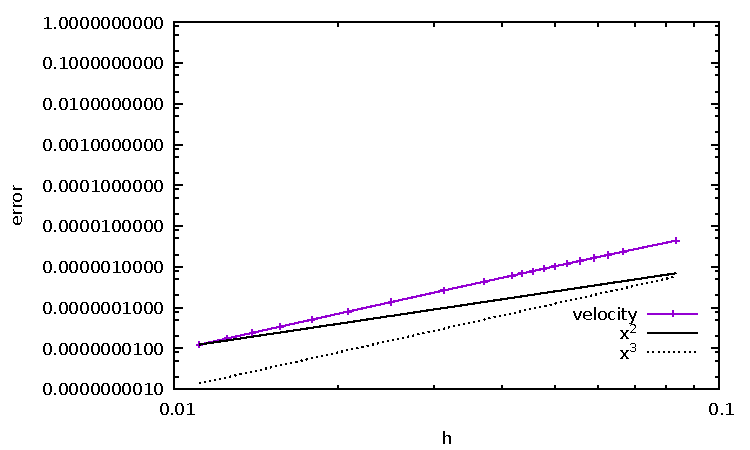
\includegraphics[width=10cm]{python_codes/fieldstone_19/errors}
\end{center}

velocity error rate is cubic, pressure superconvergent since the pressure field
is quadratic and therefore lies into the Q2 space.


\newpage
%%%%%%%%%%%%%%%%%%%%%%%%%%%%%%%%%%%%%%%%%%%%%%%%%%%%%%%%%%%%%%%%%%%%%%%%%%%%%%%%%%%%%%%%%%%%%%%%%%%%%%%%%%%%%%%%%%%%%%%
\section{{\tt fieldstone\_f15}: saddle point problem with Schur complement approach - benchmark \label{f15}}
The details of the numerical setup are presented in Section \ref{f1}.

Each element has $m_V=16$ vertices so in total $ndof_V\times m_V=32$ 
velocity dofs and 
$ndof_P*m_P=9$ pressure dofs. The total number of 
velocity dofs is therefore $NfemV=nnp \times ndofV$ while the total number of
pressure dofs is $NfemP=nel$. The total number of dofs is then $Nfem=NfemV+NfemP$.

As a consequence, matrix $\K$ has size $NfemV,NfemV$ and matrix $\G$ has size $NfemV,NfemP$.
Vector $f$ is of size $NfemV$ and vector $h$ is of size $NfemP$.  

\begin{verbatim}

60===61===62===63===64===65===66===67===68===70
||             ||             ||             ||
50   51   52   53   54   55   56   57   58   59
||             ||             ||             ||
40   41   42   43   44   45   46   47   48   49
||             ||             ||             ||
30===31===32===33===34===35===36===37===38===39
||             ||             ||             ||
20   21   22   23   24   25   26   27   28   29
||             ||             ||             ||
10   11   12   13   14   15   16   17   18   19
||             ||             ||             ||
00===01===02===03===04===05===06===07===08===09

Example of 3x2 mesh. nnx=10, nny=7, nnp=70, nelx=3, nely=2, nel=6
\end{verbatim}


\begin{verbatim}
12===13===14===15           06=====07=====08
||   ||   ||   ||           ||     ||     ||
08===09===10===11           ||     ||     ||
||   ||   ||   ||           03=====04=====05
04===05===06===07           ||     ||     ||
||   ||   ||   ||           ||     ||     ||
00===01===02===03           00=====01=====02

Velocity (Q3)               Pressure (Q2)

(r,s)_{00}=(-1,-1)          (r,s)_{00}=(-1,-1) 
(r,s)_{01}=(-1/3,-1)        (r,s)_{01}=(0,-1) 
(r,s)_{02}=(+1/3,-1)        (r,s)_{02}=(+1,-1) 
(r,s)_{03}=(+1,-1)          (r,s)_{03}=(-1,0) 
(r,s)_{04}=(-1,-1/3)        (r,s)_{04}=(0,0) 
(r,s)_{05}=(-1/3,-1/3)      (r,s)_{05}=(+1,0) 
(r,s)_{06}=(+1/3,-1/3)      (r,s)_{06}=(-1,+1) 
(r,s)_{07}=(+1,-1/3)        (r,s)_{07}=(0,+1) 
(r,s)_{08}=(-1,+1/3)        (r,s)_{08}=(+1,+1) 
(r,s)_{09}=(-1/3,+1/3)
(r,s)_{10}=(+1/3,+1/3)
(r,s)_{11}=(+1,+1/3)
(r,s)_{12}=(-1,+1)
(r,s)_{13}=(-1/3,+1)
(r,s)_{14}=(+1/3,+1)
(r,s)_{15}=(+1,+1)

\end{verbatim}







{\color{red} Write about 4 point quadrature}.








\fbox{
\parbox{10cm}{{\bf features}
\begin{itemize}
\item $Q_3\times Q_2$ element \index{$Q_3 \times Q_2$}
\item incompressible flow \index{incompressible flow}
\item mixed formulation \index{mixed formulation}
\item isothermal \index{isothermal}
\item isoviscous \index{isoviscous}
\item analytical solution \index{analytical solution}
\end{itemize}
}}

\begin{center}
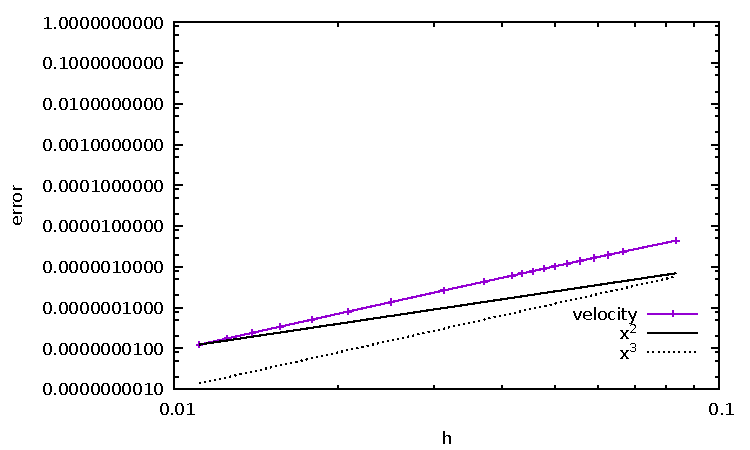
\includegraphics[width=10cm]{python_codes/fieldstone_19/errors}
\end{center}

velocity error rate is cubic, pressure superconvergent since the pressure field
is quadratic and therefore lies into the Q2 space.


\newpage
%%%%%%%%%%%%%%%%%%%%%%%%%%%%%%%%%%%%%%%%%%%%%%%%%%%%%%%%%%%%%%%%%%%%%%%%%%%%%%%%%%%%%%%%%%%%%%%%%%%%%%%%%%%%%%%%%%%%%%%
\section{{\tt fieldstone\_f16}: saddle point problem with Schur complement approach - Stokes sphere \label{f16}}
The details of the numerical setup are presented in Section \ref{f1}.

Each element has $m_V=16$ vertices so in total $ndof_V\times m_V=32$ 
velocity dofs and 
$ndof_P*m_P=9$ pressure dofs. The total number of 
velocity dofs is therefore $NfemV=nnp \times ndofV$ while the total number of
pressure dofs is $NfemP=nel$. The total number of dofs is then $Nfem=NfemV+NfemP$.

As a consequence, matrix $\K$ has size $NfemV,NfemV$ and matrix $\G$ has size $NfemV,NfemP$.
Vector $f$ is of size $NfemV$ and vector $h$ is of size $NfemP$.  

\begin{verbatim}

60===61===62===63===64===65===66===67===68===70
||             ||             ||             ||
50   51   52   53   54   55   56   57   58   59
||             ||             ||             ||
40   41   42   43   44   45   46   47   48   49
||             ||             ||             ||
30===31===32===33===34===35===36===37===38===39
||             ||             ||             ||
20   21   22   23   24   25   26   27   28   29
||             ||             ||             ||
10   11   12   13   14   15   16   17   18   19
||             ||             ||             ||
00===01===02===03===04===05===06===07===08===09

Example of 3x2 mesh. nnx=10, nny=7, nnp=70, nelx=3, nely=2, nel=6
\end{verbatim}


\begin{verbatim}
12===13===14===15           06=====07=====08
||   ||   ||   ||           ||     ||     ||
08===09===10===11           ||     ||     ||
||   ||   ||   ||           03=====04=====05
04===05===06===07           ||     ||     ||
||   ||   ||   ||           ||     ||     ||
00===01===02===03           00=====01=====02

Velocity (Q3)               Pressure (Q2)

(r,s)_{00}=(-1,-1)          (r,s)_{00}=(-1,-1) 
(r,s)_{01}=(-1/3,-1)        (r,s)_{01}=(0,-1) 
(r,s)_{02}=(+1/3,-1)        (r,s)_{02}=(+1,-1) 
(r,s)_{03}=(+1,-1)          (r,s)_{03}=(-1,0) 
(r,s)_{04}=(-1,-1/3)        (r,s)_{04}=(0,0) 
(r,s)_{05}=(-1/3,-1/3)      (r,s)_{05}=(+1,0) 
(r,s)_{06}=(+1/3,-1/3)      (r,s)_{06}=(-1,+1) 
(r,s)_{07}=(+1,-1/3)        (r,s)_{07}=(0,+1) 
(r,s)_{08}=(-1,+1/3)        (r,s)_{08}=(+1,+1) 
(r,s)_{09}=(-1/3,+1/3)
(r,s)_{10}=(+1/3,+1/3)
(r,s)_{11}=(+1,+1/3)
(r,s)_{12}=(-1,+1)
(r,s)_{13}=(-1/3,+1)
(r,s)_{14}=(+1/3,+1)
(r,s)_{15}=(+1,+1)

\end{verbatim}







{\color{red} Write about 4 point quadrature}.








\fbox{
\parbox{10cm}{{\bf features}
\begin{itemize}
\item $Q_3\times Q_2$ element \index{$Q_3 \times Q_2$}
\item incompressible flow \index{incompressible flow}
\item mixed formulation \index{mixed formulation}
\item isothermal \index{isothermal}
\item isoviscous \index{isoviscous}
\item analytical solution \index{analytical solution}
\end{itemize}
}}

\begin{center}
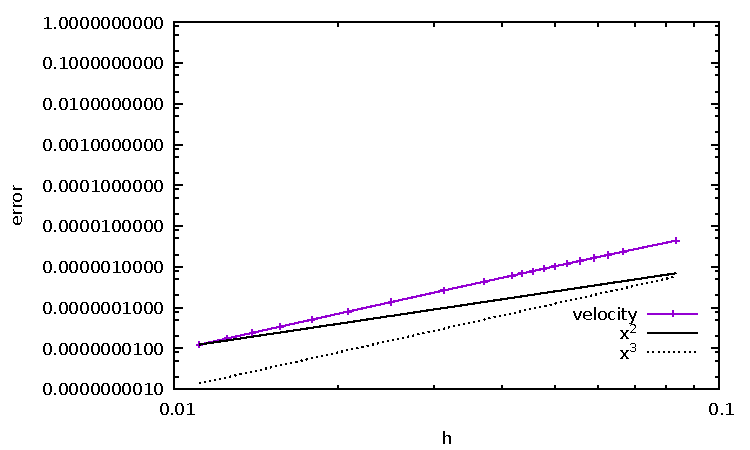
\includegraphics[width=10cm]{python_codes/fieldstone_19/errors}
\end{center}

velocity error rate is cubic, pressure superconvergent since the pressure field
is quadratic and therefore lies into the Q2 space.


\newpage
%%%%%%%%%%%%%%%%%%%%%%%%%%%%%%%%%%%%%%%%%%%%%%%%%%%%%%%%%%%%%%%%%%%%%%%%%%%%%%%
\section{{\tt fieldstone\_17}: solving the full saddle point problem in 3D \label{f17}}
The details of the numerical setup are presented in Section \ref{f1}.

Each element has $m_V=16$ vertices so in total $ndof_V\times m_V=32$ 
velocity dofs and 
$ndof_P*m_P=9$ pressure dofs. The total number of 
velocity dofs is therefore $NfemV=nnp \times ndofV$ while the total number of
pressure dofs is $NfemP=nel$. The total number of dofs is then $Nfem=NfemV+NfemP$.

As a consequence, matrix $\K$ has size $NfemV,NfemV$ and matrix $\G$ has size $NfemV,NfemP$.
Vector $f$ is of size $NfemV$ and vector $h$ is of size $NfemP$.  

\begin{verbatim}

60===61===62===63===64===65===66===67===68===70
||             ||             ||             ||
50   51   52   53   54   55   56   57   58   59
||             ||             ||             ||
40   41   42   43   44   45   46   47   48   49
||             ||             ||             ||
30===31===32===33===34===35===36===37===38===39
||             ||             ||             ||
20   21   22   23   24   25   26   27   28   29
||             ||             ||             ||
10   11   12   13   14   15   16   17   18   19
||             ||             ||             ||
00===01===02===03===04===05===06===07===08===09

Example of 3x2 mesh. nnx=10, nny=7, nnp=70, nelx=3, nely=2, nel=6
\end{verbatim}


\begin{verbatim}
12===13===14===15           06=====07=====08
||   ||   ||   ||           ||     ||     ||
08===09===10===11           ||     ||     ||
||   ||   ||   ||           03=====04=====05
04===05===06===07           ||     ||     ||
||   ||   ||   ||           ||     ||     ||
00===01===02===03           00=====01=====02

Velocity (Q3)               Pressure (Q2)

(r,s)_{00}=(-1,-1)          (r,s)_{00}=(-1,-1) 
(r,s)_{01}=(-1/3,-1)        (r,s)_{01}=(0,-1) 
(r,s)_{02}=(+1/3,-1)        (r,s)_{02}=(+1,-1) 
(r,s)_{03}=(+1,-1)          (r,s)_{03}=(-1,0) 
(r,s)_{04}=(-1,-1/3)        (r,s)_{04}=(0,0) 
(r,s)_{05}=(-1/3,-1/3)      (r,s)_{05}=(+1,0) 
(r,s)_{06}=(+1/3,-1/3)      (r,s)_{06}=(-1,+1) 
(r,s)_{07}=(+1,-1/3)        (r,s)_{07}=(0,+1) 
(r,s)_{08}=(-1,+1/3)        (r,s)_{08}=(+1,+1) 
(r,s)_{09}=(-1/3,+1/3)
(r,s)_{10}=(+1/3,+1/3)
(r,s)_{11}=(+1,+1/3)
(r,s)_{12}=(-1,+1)
(r,s)_{13}=(-1/3,+1)
(r,s)_{14}=(+1/3,+1)
(r,s)_{15}=(+1,+1)

\end{verbatim}







{\color{red} Write about 4 point quadrature}.








\fbox{
\parbox{10cm}{{\bf features}
\begin{itemize}
\item $Q_3\times Q_2$ element \index{$Q_3 \times Q_2$}
\item incompressible flow \index{incompressible flow}
\item mixed formulation \index{mixed formulation}
\item isothermal \index{isothermal}
\item isoviscous \index{isoviscous}
\item analytical solution \index{analytical solution}
\end{itemize}
}}

\begin{center}
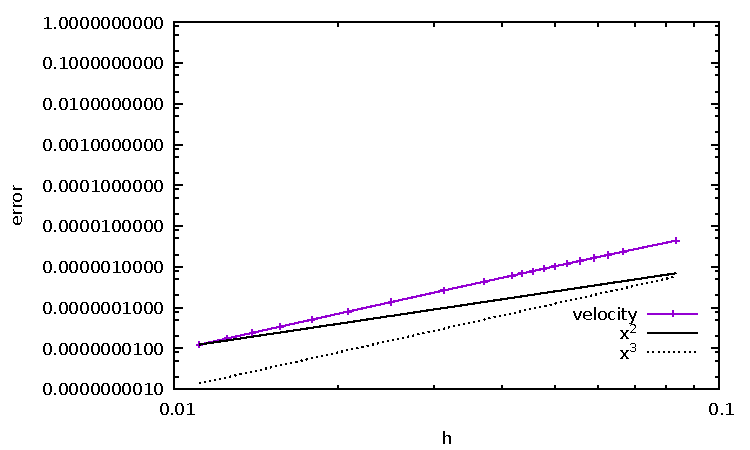
\includegraphics[width=10cm]{python_codes/fieldstone_19/errors}
\end{center}

velocity error rate is cubic, pressure superconvergent since the pressure field
is quadratic and therefore lies into the Q2 space.


\newpage
%%%%%%%%%%%%%%%%%%%%%%%%%%%%%%%%%%%%%%%%%%%%%%%%%%%%%%%%%%%%%%%%%%%%%%%%%%%%%%%
\section{{\tt fieldstone\_18}: solving the full saddle point problem with $Q_2\times Q_1$ elements \label{f18}}
The details of the numerical setup are presented in Section \ref{f1}.

Each element has $m_V=16$ vertices so in total $ndof_V\times m_V=32$ 
velocity dofs and 
$ndof_P*m_P=9$ pressure dofs. The total number of 
velocity dofs is therefore $NfemV=nnp \times ndofV$ while the total number of
pressure dofs is $NfemP=nel$. The total number of dofs is then $Nfem=NfemV+NfemP$.

As a consequence, matrix $\K$ has size $NfemV,NfemV$ and matrix $\G$ has size $NfemV,NfemP$.
Vector $f$ is of size $NfemV$ and vector $h$ is of size $NfemP$.  

\begin{verbatim}

60===61===62===63===64===65===66===67===68===70
||             ||             ||             ||
50   51   52   53   54   55   56   57   58   59
||             ||             ||             ||
40   41   42   43   44   45   46   47   48   49
||             ||             ||             ||
30===31===32===33===34===35===36===37===38===39
||             ||             ||             ||
20   21   22   23   24   25   26   27   28   29
||             ||             ||             ||
10   11   12   13   14   15   16   17   18   19
||             ||             ||             ||
00===01===02===03===04===05===06===07===08===09

Example of 3x2 mesh. nnx=10, nny=7, nnp=70, nelx=3, nely=2, nel=6
\end{verbatim}


\begin{verbatim}
12===13===14===15           06=====07=====08
||   ||   ||   ||           ||     ||     ||
08===09===10===11           ||     ||     ||
||   ||   ||   ||           03=====04=====05
04===05===06===07           ||     ||     ||
||   ||   ||   ||           ||     ||     ||
00===01===02===03           00=====01=====02

Velocity (Q3)               Pressure (Q2)

(r,s)_{00}=(-1,-1)          (r,s)_{00}=(-1,-1) 
(r,s)_{01}=(-1/3,-1)        (r,s)_{01}=(0,-1) 
(r,s)_{02}=(+1/3,-1)        (r,s)_{02}=(+1,-1) 
(r,s)_{03}=(+1,-1)          (r,s)_{03}=(-1,0) 
(r,s)_{04}=(-1,-1/3)        (r,s)_{04}=(0,0) 
(r,s)_{05}=(-1/3,-1/3)      (r,s)_{05}=(+1,0) 
(r,s)_{06}=(+1/3,-1/3)      (r,s)_{06}=(-1,+1) 
(r,s)_{07}=(+1,-1/3)        (r,s)_{07}=(0,+1) 
(r,s)_{08}=(-1,+1/3)        (r,s)_{08}=(+1,+1) 
(r,s)_{09}=(-1/3,+1/3)
(r,s)_{10}=(+1/3,+1/3)
(r,s)_{11}=(+1,+1/3)
(r,s)_{12}=(-1,+1)
(r,s)_{13}=(-1/3,+1)
(r,s)_{14}=(+1/3,+1)
(r,s)_{15}=(+1,+1)

\end{verbatim}







{\color{red} Write about 4 point quadrature}.








\fbox{
\parbox{10cm}{{\bf features}
\begin{itemize}
\item $Q_3\times Q_2$ element \index{$Q_3 \times Q_2$}
\item incompressible flow \index{incompressible flow}
\item mixed formulation \index{mixed formulation}
\item isothermal \index{isothermal}
\item isoviscous \index{isoviscous}
\item analytical solution \index{analytical solution}
\end{itemize}
}}

\begin{center}
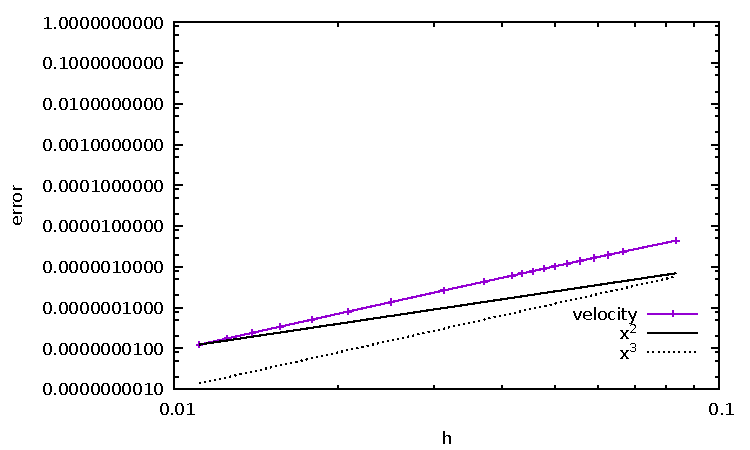
\includegraphics[width=10cm]{python_codes/fieldstone_19/errors}
\end{center}

velocity error rate is cubic, pressure superconvergent since the pressure field
is quadratic and therefore lies into the Q2 space.


\newpage
%%%%%%%%%%%%%%%%%%%%%%%%%%%%%%%%%%%%%%%%%%%%%%%%%%%%%%%%%%%%%%%%%%%%%%%%%%%%%%%
\section{{\tt fieldstone\_19}: solving the full saddle point problem with $Q_3\times Q_2$ elements \label{f19}}
The details of the numerical setup are presented in Section \ref{f1}.

Each element has $m_V=16$ vertices so in total $ndof_V\times m_V=32$ 
velocity dofs and 
$ndof_P*m_P=9$ pressure dofs. The total number of 
velocity dofs is therefore $NfemV=nnp \times ndofV$ while the total number of
pressure dofs is $NfemP=nel$. The total number of dofs is then $Nfem=NfemV+NfemP$.

As a consequence, matrix $\K$ has size $NfemV,NfemV$ and matrix $\G$ has size $NfemV,NfemP$.
Vector $f$ is of size $NfemV$ and vector $h$ is of size $NfemP$.  

\begin{verbatim}

60===61===62===63===64===65===66===67===68===70
||             ||             ||             ||
50   51   52   53   54   55   56   57   58   59
||             ||             ||             ||
40   41   42   43   44   45   46   47   48   49
||             ||             ||             ||
30===31===32===33===34===35===36===37===38===39
||             ||             ||             ||
20   21   22   23   24   25   26   27   28   29
||             ||             ||             ||
10   11   12   13   14   15   16   17   18   19
||             ||             ||             ||
00===01===02===03===04===05===06===07===08===09

Example of 3x2 mesh. nnx=10, nny=7, nnp=70, nelx=3, nely=2, nel=6
\end{verbatim}


\begin{verbatim}
12===13===14===15           06=====07=====08
||   ||   ||   ||           ||     ||     ||
08===09===10===11           ||     ||     ||
||   ||   ||   ||           03=====04=====05
04===05===06===07           ||     ||     ||
||   ||   ||   ||           ||     ||     ||
00===01===02===03           00=====01=====02

Velocity (Q3)               Pressure (Q2)

(r,s)_{00}=(-1,-1)          (r,s)_{00}=(-1,-1) 
(r,s)_{01}=(-1/3,-1)        (r,s)_{01}=(0,-1) 
(r,s)_{02}=(+1/3,-1)        (r,s)_{02}=(+1,-1) 
(r,s)_{03}=(+1,-1)          (r,s)_{03}=(-1,0) 
(r,s)_{04}=(-1,-1/3)        (r,s)_{04}=(0,0) 
(r,s)_{05}=(-1/3,-1/3)      (r,s)_{05}=(+1,0) 
(r,s)_{06}=(+1/3,-1/3)      (r,s)_{06}=(-1,+1) 
(r,s)_{07}=(+1,-1/3)        (r,s)_{07}=(0,+1) 
(r,s)_{08}=(-1,+1/3)        (r,s)_{08}=(+1,+1) 
(r,s)_{09}=(-1/3,+1/3)
(r,s)_{10}=(+1/3,+1/3)
(r,s)_{11}=(+1,+1/3)
(r,s)_{12}=(-1,+1)
(r,s)_{13}=(-1/3,+1)
(r,s)_{14}=(+1/3,+1)
(r,s)_{15}=(+1,+1)

\end{verbatim}







{\color{red} Write about 4 point quadrature}.








\fbox{
\parbox{10cm}{{\bf features}
\begin{itemize}
\item $Q_3\times Q_2$ element \index{$Q_3 \times Q_2$}
\item incompressible flow \index{incompressible flow}
\item mixed formulation \index{mixed formulation}
\item isothermal \index{isothermal}
\item isoviscous \index{isoviscous}
\item analytical solution \index{analytical solution}
\end{itemize}
}}

\begin{center}
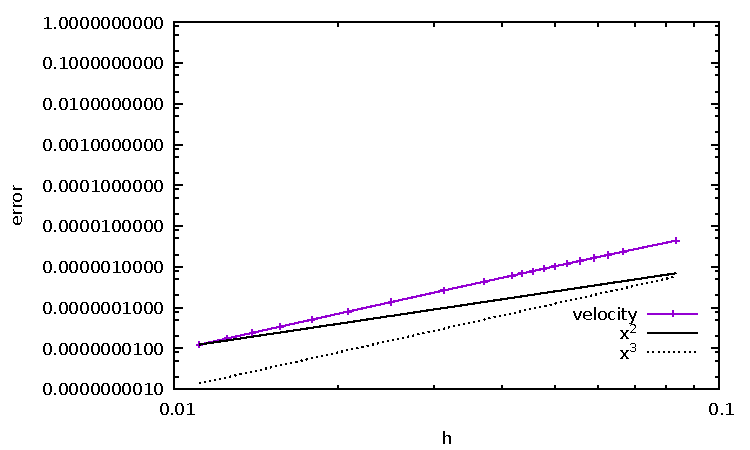
\includegraphics[width=10cm]{python_codes/fieldstone_19/errors}
\end{center}

velocity error rate is cubic, pressure superconvergent since the pressure field
is quadratic and therefore lies into the Q2 space.


\newpage
%%%%%%%%%%%%%%%%%%%%%%%%%%%%%%%%%%%%%%%%%%%%%%%%%%%%%%%%%%%%%%%%%%%%%%%%%%%%%%%
\section{{\tt fieldstone\_20}: the Busse benchmark \label{f20}}
The details of the numerical setup are presented in Section \ref{f1}.

Each element has $m_V=16$ vertices so in total $ndof_V\times m_V=32$ 
velocity dofs and 
$ndof_P*m_P=9$ pressure dofs. The total number of 
velocity dofs is therefore $NfemV=nnp \times ndofV$ while the total number of
pressure dofs is $NfemP=nel$. The total number of dofs is then $Nfem=NfemV+NfemP$.

As a consequence, matrix $\K$ has size $NfemV,NfemV$ and matrix $\G$ has size $NfemV,NfemP$.
Vector $f$ is of size $NfemV$ and vector $h$ is of size $NfemP$.  

\begin{verbatim}

60===61===62===63===64===65===66===67===68===70
||             ||             ||             ||
50   51   52   53   54   55   56   57   58   59
||             ||             ||             ||
40   41   42   43   44   45   46   47   48   49
||             ||             ||             ||
30===31===32===33===34===35===36===37===38===39
||             ||             ||             ||
20   21   22   23   24   25   26   27   28   29
||             ||             ||             ||
10   11   12   13   14   15   16   17   18   19
||             ||             ||             ||
00===01===02===03===04===05===06===07===08===09

Example of 3x2 mesh. nnx=10, nny=7, nnp=70, nelx=3, nely=2, nel=6
\end{verbatim}


\begin{verbatim}
12===13===14===15           06=====07=====08
||   ||   ||   ||           ||     ||     ||
08===09===10===11           ||     ||     ||
||   ||   ||   ||           03=====04=====05
04===05===06===07           ||     ||     ||
||   ||   ||   ||           ||     ||     ||
00===01===02===03           00=====01=====02

Velocity (Q3)               Pressure (Q2)

(r,s)_{00}=(-1,-1)          (r,s)_{00}=(-1,-1) 
(r,s)_{01}=(-1/3,-1)        (r,s)_{01}=(0,-1) 
(r,s)_{02}=(+1/3,-1)        (r,s)_{02}=(+1,-1) 
(r,s)_{03}=(+1,-1)          (r,s)_{03}=(-1,0) 
(r,s)_{04}=(-1,-1/3)        (r,s)_{04}=(0,0) 
(r,s)_{05}=(-1/3,-1/3)      (r,s)_{05}=(+1,0) 
(r,s)_{06}=(+1/3,-1/3)      (r,s)_{06}=(-1,+1) 
(r,s)_{07}=(+1,-1/3)        (r,s)_{07}=(0,+1) 
(r,s)_{08}=(-1,+1/3)        (r,s)_{08}=(+1,+1) 
(r,s)_{09}=(-1/3,+1/3)
(r,s)_{10}=(+1/3,+1/3)
(r,s)_{11}=(+1,+1/3)
(r,s)_{12}=(-1,+1)
(r,s)_{13}=(-1/3,+1)
(r,s)_{14}=(+1/3,+1)
(r,s)_{15}=(+1,+1)

\end{verbatim}







{\color{red} Write about 4 point quadrature}.








\fbox{
\parbox{10cm}{{\bf features}
\begin{itemize}
\item $Q_3\times Q_2$ element \index{$Q_3 \times Q_2$}
\item incompressible flow \index{incompressible flow}
\item mixed formulation \index{mixed formulation}
\item isothermal \index{isothermal}
\item isoviscous \index{isoviscous}
\item analytical solution \index{analytical solution}
\end{itemize}
}}

\begin{center}
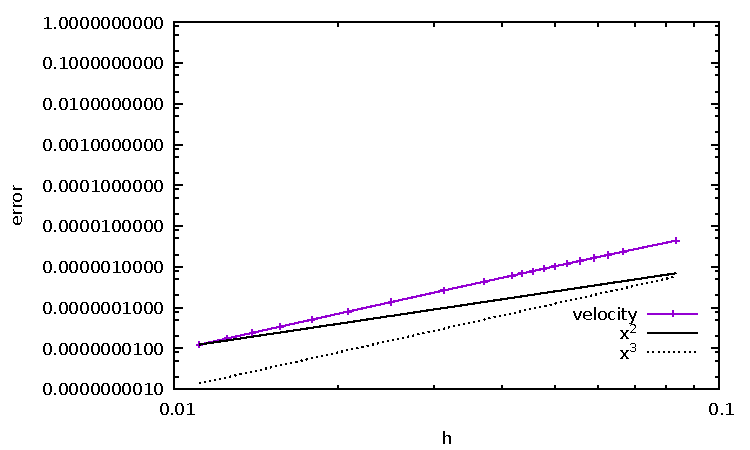
\includegraphics[width=10cm]{python_codes/fieldstone_19/errors}
\end{center}

velocity error rate is cubic, pressure superconvergent since the pressure field
is quadratic and therefore lies into the Q2 space.


\newpage
%%%%%%%%%%%%%%%%%%%%%%%%%%%%%%%%%%%%%%%%%%%%%%%%%%%%%%%%%%%%%%%%%%%%%%%%%%%%%%%
\section{{\tt fieldstone\_21}: The non-conforming $Q_1 \times P_0$ element \label{f21}}
The details of the numerical setup are presented in Section \ref{f1}.

Each element has $m_V=16$ vertices so in total $ndof_V\times m_V=32$ 
velocity dofs and 
$ndof_P*m_P=9$ pressure dofs. The total number of 
velocity dofs is therefore $NfemV=nnp \times ndofV$ while the total number of
pressure dofs is $NfemP=nel$. The total number of dofs is then $Nfem=NfemV+NfemP$.

As a consequence, matrix $\K$ has size $NfemV,NfemV$ and matrix $\G$ has size $NfemV,NfemP$.
Vector $f$ is of size $NfemV$ and vector $h$ is of size $NfemP$.  

\begin{verbatim}

60===61===62===63===64===65===66===67===68===70
||             ||             ||             ||
50   51   52   53   54   55   56   57   58   59
||             ||             ||             ||
40   41   42   43   44   45   46   47   48   49
||             ||             ||             ||
30===31===32===33===34===35===36===37===38===39
||             ||             ||             ||
20   21   22   23   24   25   26   27   28   29
||             ||             ||             ||
10   11   12   13   14   15   16   17   18   19
||             ||             ||             ||
00===01===02===03===04===05===06===07===08===09

Example of 3x2 mesh. nnx=10, nny=7, nnp=70, nelx=3, nely=2, nel=6
\end{verbatim}


\begin{verbatim}
12===13===14===15           06=====07=====08
||   ||   ||   ||           ||     ||     ||
08===09===10===11           ||     ||     ||
||   ||   ||   ||           03=====04=====05
04===05===06===07           ||     ||     ||
||   ||   ||   ||           ||     ||     ||
00===01===02===03           00=====01=====02

Velocity (Q3)               Pressure (Q2)

(r,s)_{00}=(-1,-1)          (r,s)_{00}=(-1,-1) 
(r,s)_{01}=(-1/3,-1)        (r,s)_{01}=(0,-1) 
(r,s)_{02}=(+1/3,-1)        (r,s)_{02}=(+1,-1) 
(r,s)_{03}=(+1,-1)          (r,s)_{03}=(-1,0) 
(r,s)_{04}=(-1,-1/3)        (r,s)_{04}=(0,0) 
(r,s)_{05}=(-1/3,-1/3)      (r,s)_{05}=(+1,0) 
(r,s)_{06}=(+1/3,-1/3)      (r,s)_{06}=(-1,+1) 
(r,s)_{07}=(+1,-1/3)        (r,s)_{07}=(0,+1) 
(r,s)_{08}=(-1,+1/3)        (r,s)_{08}=(+1,+1) 
(r,s)_{09}=(-1/3,+1/3)
(r,s)_{10}=(+1/3,+1/3)
(r,s)_{11}=(+1,+1/3)
(r,s)_{12}=(-1,+1)
(r,s)_{13}=(-1/3,+1)
(r,s)_{14}=(+1/3,+1)
(r,s)_{15}=(+1,+1)

\end{verbatim}







{\color{red} Write about 4 point quadrature}.








\fbox{
\parbox{10cm}{{\bf features}
\begin{itemize}
\item $Q_3\times Q_2$ element \index{$Q_3 \times Q_2$}
\item incompressible flow \index{incompressible flow}
\item mixed formulation \index{mixed formulation}
\item isothermal \index{isothermal}
\item isoviscous \index{isoviscous}
\item analytical solution \index{analytical solution}
\end{itemize}
}}

\begin{center}
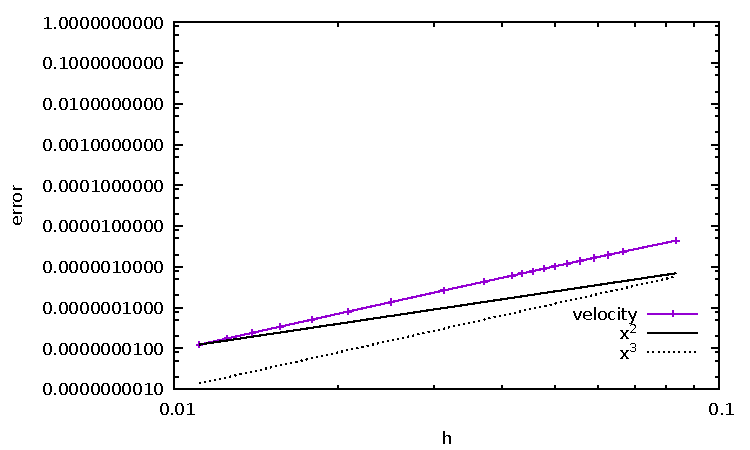
\includegraphics[width=10cm]{python_codes/fieldstone_19/errors}
\end{center}

velocity error rate is cubic, pressure superconvergent since the pressure field
is quadratic and therefore lies into the Q2 space.


\newpage
%%%%%%%%%%%%%%%%%%%%%%%%%%%%%%%%%%%%%%%%%%%%%%%%%%%%%%%%%%%%%%%%%%%%%%%%%%%%%%%
\section{{\tt fieldstone\_22}: The stabilised $Q_1 \times Q_1$ element \label{f22}} 
The details of the numerical setup are presented in Section \ref{f1}.

Each element has $m_V=16$ vertices so in total $ndof_V\times m_V=32$ 
velocity dofs and 
$ndof_P*m_P=9$ pressure dofs. The total number of 
velocity dofs is therefore $NfemV=nnp \times ndofV$ while the total number of
pressure dofs is $NfemP=nel$. The total number of dofs is then $Nfem=NfemV+NfemP$.

As a consequence, matrix $\K$ has size $NfemV,NfemV$ and matrix $\G$ has size $NfemV,NfemP$.
Vector $f$ is of size $NfemV$ and vector $h$ is of size $NfemP$.  

\begin{verbatim}

60===61===62===63===64===65===66===67===68===70
||             ||             ||             ||
50   51   52   53   54   55   56   57   58   59
||             ||             ||             ||
40   41   42   43   44   45   46   47   48   49
||             ||             ||             ||
30===31===32===33===34===35===36===37===38===39
||             ||             ||             ||
20   21   22   23   24   25   26   27   28   29
||             ||             ||             ||
10   11   12   13   14   15   16   17   18   19
||             ||             ||             ||
00===01===02===03===04===05===06===07===08===09

Example of 3x2 mesh. nnx=10, nny=7, nnp=70, nelx=3, nely=2, nel=6
\end{verbatim}


\begin{verbatim}
12===13===14===15           06=====07=====08
||   ||   ||   ||           ||     ||     ||
08===09===10===11           ||     ||     ||
||   ||   ||   ||           03=====04=====05
04===05===06===07           ||     ||     ||
||   ||   ||   ||           ||     ||     ||
00===01===02===03           00=====01=====02

Velocity (Q3)               Pressure (Q2)

(r,s)_{00}=(-1,-1)          (r,s)_{00}=(-1,-1) 
(r,s)_{01}=(-1/3,-1)        (r,s)_{01}=(0,-1) 
(r,s)_{02}=(+1/3,-1)        (r,s)_{02}=(+1,-1) 
(r,s)_{03}=(+1,-1)          (r,s)_{03}=(-1,0) 
(r,s)_{04}=(-1,-1/3)        (r,s)_{04}=(0,0) 
(r,s)_{05}=(-1/3,-1/3)      (r,s)_{05}=(+1,0) 
(r,s)_{06}=(+1/3,-1/3)      (r,s)_{06}=(-1,+1) 
(r,s)_{07}=(+1,-1/3)        (r,s)_{07}=(0,+1) 
(r,s)_{08}=(-1,+1/3)        (r,s)_{08}=(+1,+1) 
(r,s)_{09}=(-1/3,+1/3)
(r,s)_{10}=(+1/3,+1/3)
(r,s)_{11}=(+1,+1/3)
(r,s)_{12}=(-1,+1)
(r,s)_{13}=(-1/3,+1)
(r,s)_{14}=(+1/3,+1)
(r,s)_{15}=(+1,+1)

\end{verbatim}







{\color{red} Write about 4 point quadrature}.








\fbox{
\parbox{10cm}{{\bf features}
\begin{itemize}
\item $Q_3\times Q_2$ element \index{$Q_3 \times Q_2$}
\item incompressible flow \index{incompressible flow}
\item mixed formulation \index{mixed formulation}
\item isothermal \index{isothermal}
\item isoviscous \index{isoviscous}
\item analytical solution \index{analytical solution}
\end{itemize}
}}

\begin{center}
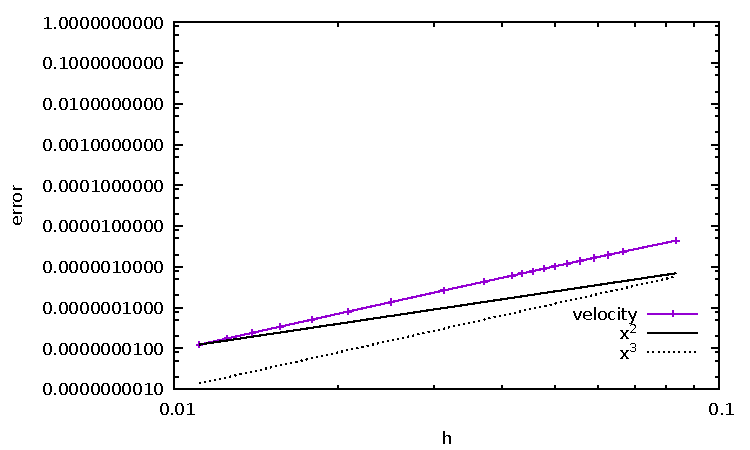
\includegraphics[width=10cm]{python_codes/fieldstone_19/errors}
\end{center}

velocity error rate is cubic, pressure superconvergent since the pressure field
is quadratic and therefore lies into the Q2 space.


\newpage
%%%%%%%%%%%%%%%%%%%%%%%%%%%%%%%%%%%%%%%%%%%%%%%%%%%%%%%%%%%%%%%%%%%%%%%%%%%%%%%
\section{{\tt fieldstone\_23}: compressible flow (1) - analytical benchmark \label{f23}}
The details of the numerical setup are presented in Section \ref{f1}.

Each element has $m_V=16$ vertices so in total $ndof_V\times m_V=32$ 
velocity dofs and 
$ndof_P*m_P=9$ pressure dofs. The total number of 
velocity dofs is therefore $NfemV=nnp \times ndofV$ while the total number of
pressure dofs is $NfemP=nel$. The total number of dofs is then $Nfem=NfemV+NfemP$.

As a consequence, matrix $\K$ has size $NfemV,NfemV$ and matrix $\G$ has size $NfemV,NfemP$.
Vector $f$ is of size $NfemV$ and vector $h$ is of size $NfemP$.  

\begin{verbatim}

60===61===62===63===64===65===66===67===68===70
||             ||             ||             ||
50   51   52   53   54   55   56   57   58   59
||             ||             ||             ||
40   41   42   43   44   45   46   47   48   49
||             ||             ||             ||
30===31===32===33===34===35===36===37===38===39
||             ||             ||             ||
20   21   22   23   24   25   26   27   28   29
||             ||             ||             ||
10   11   12   13   14   15   16   17   18   19
||             ||             ||             ||
00===01===02===03===04===05===06===07===08===09

Example of 3x2 mesh. nnx=10, nny=7, nnp=70, nelx=3, nely=2, nel=6
\end{verbatim}


\begin{verbatim}
12===13===14===15           06=====07=====08
||   ||   ||   ||           ||     ||     ||
08===09===10===11           ||     ||     ||
||   ||   ||   ||           03=====04=====05
04===05===06===07           ||     ||     ||
||   ||   ||   ||           ||     ||     ||
00===01===02===03           00=====01=====02

Velocity (Q3)               Pressure (Q2)

(r,s)_{00}=(-1,-1)          (r,s)_{00}=(-1,-1) 
(r,s)_{01}=(-1/3,-1)        (r,s)_{01}=(0,-1) 
(r,s)_{02}=(+1/3,-1)        (r,s)_{02}=(+1,-1) 
(r,s)_{03}=(+1,-1)          (r,s)_{03}=(-1,0) 
(r,s)_{04}=(-1,-1/3)        (r,s)_{04}=(0,0) 
(r,s)_{05}=(-1/3,-1/3)      (r,s)_{05}=(+1,0) 
(r,s)_{06}=(+1/3,-1/3)      (r,s)_{06}=(-1,+1) 
(r,s)_{07}=(+1,-1/3)        (r,s)_{07}=(0,+1) 
(r,s)_{08}=(-1,+1/3)        (r,s)_{08}=(+1,+1) 
(r,s)_{09}=(-1/3,+1/3)
(r,s)_{10}=(+1/3,+1/3)
(r,s)_{11}=(+1,+1/3)
(r,s)_{12}=(-1,+1)
(r,s)_{13}=(-1/3,+1)
(r,s)_{14}=(+1/3,+1)
(r,s)_{15}=(+1,+1)

\end{verbatim}







{\color{red} Write about 4 point quadrature}.








\fbox{
\parbox{10cm}{{\bf features}
\begin{itemize}
\item $Q_3\times Q_2$ element \index{$Q_3 \times Q_2$}
\item incompressible flow \index{incompressible flow}
\item mixed formulation \index{mixed formulation}
\item isothermal \index{isothermal}
\item isoviscous \index{isoviscous}
\item analytical solution \index{analytical solution}
\end{itemize}
}}

\begin{center}
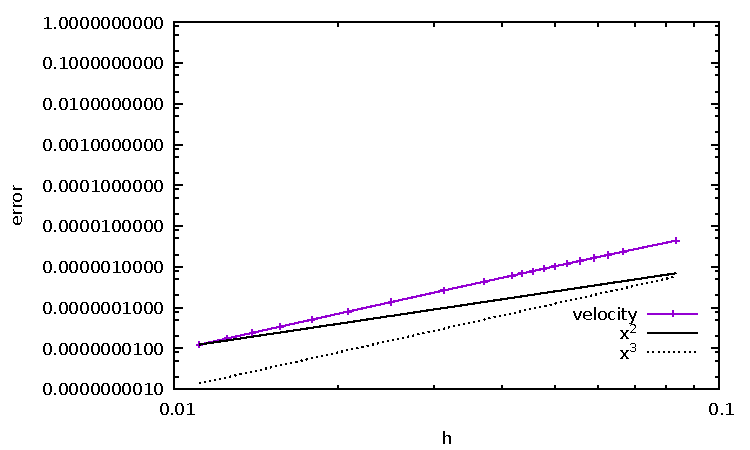
\includegraphics[width=10cm]{python_codes/fieldstone_19/errors}
\end{center}

velocity error rate is cubic, pressure superconvergent since the pressure field
is quadratic and therefore lies into the Q2 space.


\newpage
%%%%%%%%%%%%%%%%%%%%%%%%%%%%%%%%%%%%%%%%%%%%%%%%%%%%%%%%%%%%%%%%%%%%%%%%%%%%%%%
\section{{\tt fieldstone\_24}: compressible flow (2) - convection box \label{f24}}
The details of the numerical setup are presented in Section \ref{f1}.

Each element has $m_V=16$ vertices so in total $ndof_V\times m_V=32$ 
velocity dofs and 
$ndof_P*m_P=9$ pressure dofs. The total number of 
velocity dofs is therefore $NfemV=nnp \times ndofV$ while the total number of
pressure dofs is $NfemP=nel$. The total number of dofs is then $Nfem=NfemV+NfemP$.

As a consequence, matrix $\K$ has size $NfemV,NfemV$ and matrix $\G$ has size $NfemV,NfemP$.
Vector $f$ is of size $NfemV$ and vector $h$ is of size $NfemP$.  

\begin{verbatim}

60===61===62===63===64===65===66===67===68===70
||             ||             ||             ||
50   51   52   53   54   55   56   57   58   59
||             ||             ||             ||
40   41   42   43   44   45   46   47   48   49
||             ||             ||             ||
30===31===32===33===34===35===36===37===38===39
||             ||             ||             ||
20   21   22   23   24   25   26   27   28   29
||             ||             ||             ||
10   11   12   13   14   15   16   17   18   19
||             ||             ||             ||
00===01===02===03===04===05===06===07===08===09

Example of 3x2 mesh. nnx=10, nny=7, nnp=70, nelx=3, nely=2, nel=6
\end{verbatim}


\begin{verbatim}
12===13===14===15           06=====07=====08
||   ||   ||   ||           ||     ||     ||
08===09===10===11           ||     ||     ||
||   ||   ||   ||           03=====04=====05
04===05===06===07           ||     ||     ||
||   ||   ||   ||           ||     ||     ||
00===01===02===03           00=====01=====02

Velocity (Q3)               Pressure (Q2)

(r,s)_{00}=(-1,-1)          (r,s)_{00}=(-1,-1) 
(r,s)_{01}=(-1/3,-1)        (r,s)_{01}=(0,-1) 
(r,s)_{02}=(+1/3,-1)        (r,s)_{02}=(+1,-1) 
(r,s)_{03}=(+1,-1)          (r,s)_{03}=(-1,0) 
(r,s)_{04}=(-1,-1/3)        (r,s)_{04}=(0,0) 
(r,s)_{05}=(-1/3,-1/3)      (r,s)_{05}=(+1,0) 
(r,s)_{06}=(+1/3,-1/3)      (r,s)_{06}=(-1,+1) 
(r,s)_{07}=(+1,-1/3)        (r,s)_{07}=(0,+1) 
(r,s)_{08}=(-1,+1/3)        (r,s)_{08}=(+1,+1) 
(r,s)_{09}=(-1/3,+1/3)
(r,s)_{10}=(+1/3,+1/3)
(r,s)_{11}=(+1,+1/3)
(r,s)_{12}=(-1,+1)
(r,s)_{13}=(-1/3,+1)
(r,s)_{14}=(+1/3,+1)
(r,s)_{15}=(+1,+1)

\end{verbatim}







{\color{red} Write about 4 point quadrature}.








\fbox{
\parbox{10cm}{{\bf features}
\begin{itemize}
\item $Q_3\times Q_2$ element \index{$Q_3 \times Q_2$}
\item incompressible flow \index{incompressible flow}
\item mixed formulation \index{mixed formulation}
\item isothermal \index{isothermal}
\item isoviscous \index{isoviscous}
\item analytical solution \index{analytical solution}
\end{itemize}
}}

\begin{center}
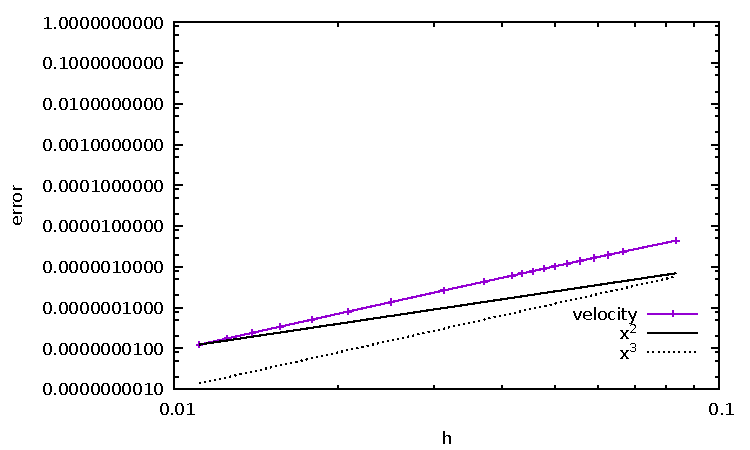
\includegraphics[width=10cm]{python_codes/fieldstone_19/errors}
\end{center}

velocity error rate is cubic, pressure superconvergent since the pressure field
is quadratic and therefore lies into the Q2 space.


\newpage
%%%%%%%%%%%%%%%%%%%%%%%%%%%%%%%%%%%%%%%%%%%%%%%%%%%%%%%%%%%%%%%%%%%%%%%%%%%%%%%
\section{{\tt fieldstone\_25}: Rayleigh-Taylor instability (1) - instantaneous \label{f25}}
The details of the numerical setup are presented in Section \ref{f1}.

Each element has $m_V=16$ vertices so in total $ndof_V\times m_V=32$ 
velocity dofs and 
$ndof_P*m_P=9$ pressure dofs. The total number of 
velocity dofs is therefore $NfemV=nnp \times ndofV$ while the total number of
pressure dofs is $NfemP=nel$. The total number of dofs is then $Nfem=NfemV+NfemP$.

As a consequence, matrix $\K$ has size $NfemV,NfemV$ and matrix $\G$ has size $NfemV,NfemP$.
Vector $f$ is of size $NfemV$ and vector $h$ is of size $NfemP$.  

\begin{verbatim}

60===61===62===63===64===65===66===67===68===70
||             ||             ||             ||
50   51   52   53   54   55   56   57   58   59
||             ||             ||             ||
40   41   42   43   44   45   46   47   48   49
||             ||             ||             ||
30===31===32===33===34===35===36===37===38===39
||             ||             ||             ||
20   21   22   23   24   25   26   27   28   29
||             ||             ||             ||
10   11   12   13   14   15   16   17   18   19
||             ||             ||             ||
00===01===02===03===04===05===06===07===08===09

Example of 3x2 mesh. nnx=10, nny=7, nnp=70, nelx=3, nely=2, nel=6
\end{verbatim}


\begin{verbatim}
12===13===14===15           06=====07=====08
||   ||   ||   ||           ||     ||     ||
08===09===10===11           ||     ||     ||
||   ||   ||   ||           03=====04=====05
04===05===06===07           ||     ||     ||
||   ||   ||   ||           ||     ||     ||
00===01===02===03           00=====01=====02

Velocity (Q3)               Pressure (Q2)

(r,s)_{00}=(-1,-1)          (r,s)_{00}=(-1,-1) 
(r,s)_{01}=(-1/3,-1)        (r,s)_{01}=(0,-1) 
(r,s)_{02}=(+1/3,-1)        (r,s)_{02}=(+1,-1) 
(r,s)_{03}=(+1,-1)          (r,s)_{03}=(-1,0) 
(r,s)_{04}=(-1,-1/3)        (r,s)_{04}=(0,0) 
(r,s)_{05}=(-1/3,-1/3)      (r,s)_{05}=(+1,0) 
(r,s)_{06}=(+1/3,-1/3)      (r,s)_{06}=(-1,+1) 
(r,s)_{07}=(+1,-1/3)        (r,s)_{07}=(0,+1) 
(r,s)_{08}=(-1,+1/3)        (r,s)_{08}=(+1,+1) 
(r,s)_{09}=(-1/3,+1/3)
(r,s)_{10}=(+1/3,+1/3)
(r,s)_{11}=(+1,+1/3)
(r,s)_{12}=(-1,+1)
(r,s)_{13}=(-1/3,+1)
(r,s)_{14}=(+1/3,+1)
(r,s)_{15}=(+1,+1)

\end{verbatim}







{\color{red} Write about 4 point quadrature}.








\fbox{
\parbox{10cm}{{\bf features}
\begin{itemize}
\item $Q_3\times Q_2$ element \index{$Q_3 \times Q_2$}
\item incompressible flow \index{incompressible flow}
\item mixed formulation \index{mixed formulation}
\item isothermal \index{isothermal}
\item isoviscous \index{isoviscous}
\item analytical solution \index{analytical solution}
\end{itemize}
}}

\begin{center}
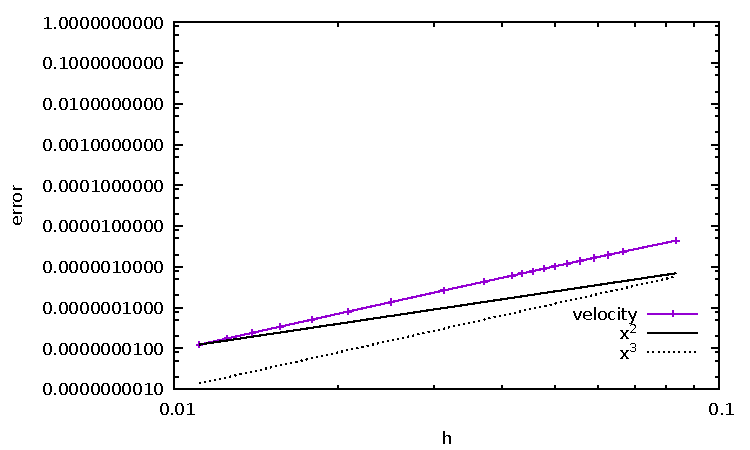
\includegraphics[width=10cm]{python_codes/fieldstone_19/errors}
\end{center}

velocity error rate is cubic, pressure superconvergent since the pressure field
is quadratic and therefore lies into the Q2 space.


\newpage
%%%%%%%%%%%%%%%%%%%%%%%%%%%%%%%%%%%%%%%%%%%%%%%%%%%%%%%%%%%%%%%%%%%%%%%%%%%%%%%
\section{{\tt fieldstone\_26}: Slab detachment benchmark (1) - instantaneous \label{f26}}
The details of the numerical setup are presented in Section \ref{f1}.

Each element has $m_V=16$ vertices so in total $ndof_V\times m_V=32$ 
velocity dofs and 
$ndof_P*m_P=9$ pressure dofs. The total number of 
velocity dofs is therefore $NfemV=nnp \times ndofV$ while the total number of
pressure dofs is $NfemP=nel$. The total number of dofs is then $Nfem=NfemV+NfemP$.

As a consequence, matrix $\K$ has size $NfemV,NfemV$ and matrix $\G$ has size $NfemV,NfemP$.
Vector $f$ is of size $NfemV$ and vector $h$ is of size $NfemP$.  

\begin{verbatim}

60===61===62===63===64===65===66===67===68===70
||             ||             ||             ||
50   51   52   53   54   55   56   57   58   59
||             ||             ||             ||
40   41   42   43   44   45   46   47   48   49
||             ||             ||             ||
30===31===32===33===34===35===36===37===38===39
||             ||             ||             ||
20   21   22   23   24   25   26   27   28   29
||             ||             ||             ||
10   11   12   13   14   15   16   17   18   19
||             ||             ||             ||
00===01===02===03===04===05===06===07===08===09

Example of 3x2 mesh. nnx=10, nny=7, nnp=70, nelx=3, nely=2, nel=6
\end{verbatim}


\begin{verbatim}
12===13===14===15           06=====07=====08
||   ||   ||   ||           ||     ||     ||
08===09===10===11           ||     ||     ||
||   ||   ||   ||           03=====04=====05
04===05===06===07           ||     ||     ||
||   ||   ||   ||           ||     ||     ||
00===01===02===03           00=====01=====02

Velocity (Q3)               Pressure (Q2)

(r,s)_{00}=(-1,-1)          (r,s)_{00}=(-1,-1) 
(r,s)_{01}=(-1/3,-1)        (r,s)_{01}=(0,-1) 
(r,s)_{02}=(+1/3,-1)        (r,s)_{02}=(+1,-1) 
(r,s)_{03}=(+1,-1)          (r,s)_{03}=(-1,0) 
(r,s)_{04}=(-1,-1/3)        (r,s)_{04}=(0,0) 
(r,s)_{05}=(-1/3,-1/3)      (r,s)_{05}=(+1,0) 
(r,s)_{06}=(+1/3,-1/3)      (r,s)_{06}=(-1,+1) 
(r,s)_{07}=(+1,-1/3)        (r,s)_{07}=(0,+1) 
(r,s)_{08}=(-1,+1/3)        (r,s)_{08}=(+1,+1) 
(r,s)_{09}=(-1/3,+1/3)
(r,s)_{10}=(+1/3,+1/3)
(r,s)_{11}=(+1,+1/3)
(r,s)_{12}=(-1,+1)
(r,s)_{13}=(-1/3,+1)
(r,s)_{14}=(+1/3,+1)
(r,s)_{15}=(+1,+1)

\end{verbatim}







{\color{red} Write about 4 point quadrature}.








\fbox{
\parbox{10cm}{{\bf features}
\begin{itemize}
\item $Q_3\times Q_2$ element \index{$Q_3 \times Q_2$}
\item incompressible flow \index{incompressible flow}
\item mixed formulation \index{mixed formulation}
\item isothermal \index{isothermal}
\item isoviscous \index{isoviscous}
\item analytical solution \index{analytical solution}
\end{itemize}
}}

\begin{center}
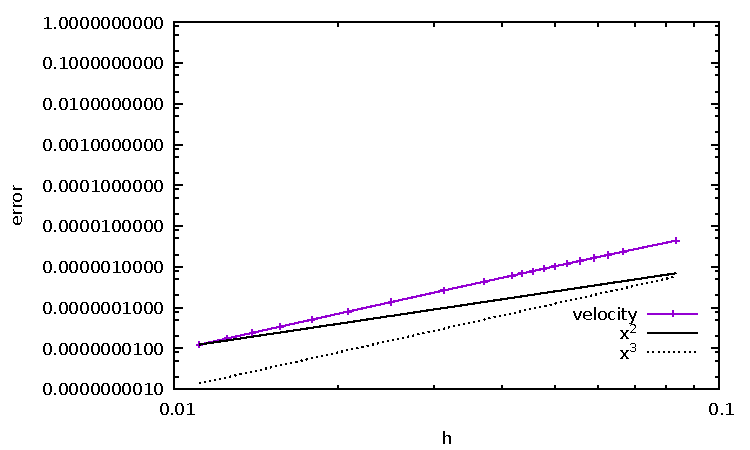
\includegraphics[width=10cm]{python_codes/fieldstone_19/errors}
\end{center}

velocity error rate is cubic, pressure superconvergent since the pressure field
is quadratic and therefore lies into the Q2 space.


\newpage
%%%%%%%%%%%%%%%%%%%%%%%%%%%%%%%%%%%%%%%%%%%%%%%%%%%%%%%%%%%%%%%%%%%%%%%%%%%%%%%
\section{{\tt fieldstone\_27}: Consistent Boundary Flux \label{f27}}
In what follows we will be re-doing the numerical experiments presented in 
Zhong et al. \cite{zhgh93}.

The first benchmark showcases a unit square domain with free slip 
boundary conditions prescribed on all sides.
The resolution is fixed to 64x64 $Q_1 \times P_0$ elements. 
The flow is isoviscous and the buoyancy force is given by 
\begin{eqnarray}
f_x &=& 0 \nonumber\\
f_y &=& \rho \alpha T(x,y) \nonumber
\end{eqnarray}
with the temperature field given by 
\[
T(x,y) = \cos(kx) \delta(y-y_0)
\]
where $k=2\pi/\lambda$ and $\lambda$ is a wavelength, 
and $y_0$ represents the location of the buoyancy.

One can prove (\cite{zhgh93} and refs. therein) that 
there is an analytic solution for the surface stress $\sigma_{zz}$:
\[
\frac{\sigma_{yy}}{\rho \alpha g} =
\frac{\cos (kx)}{\sinh^2(k)}
\left[
k(1-y_0)\sinh(k) \cosh(ky_0)-k \sinh(k(1-y_0))
+\sinh(k) \sinh(ky_0)
\right]
\]

{\bf Remark}: This is suspicious since $\rho \alpha g$ does not have the 
dimensions of a stress! Instead we shall use $\rho \alpha g h$, and choosing 
where $h$ is the element size.

\begin{center}
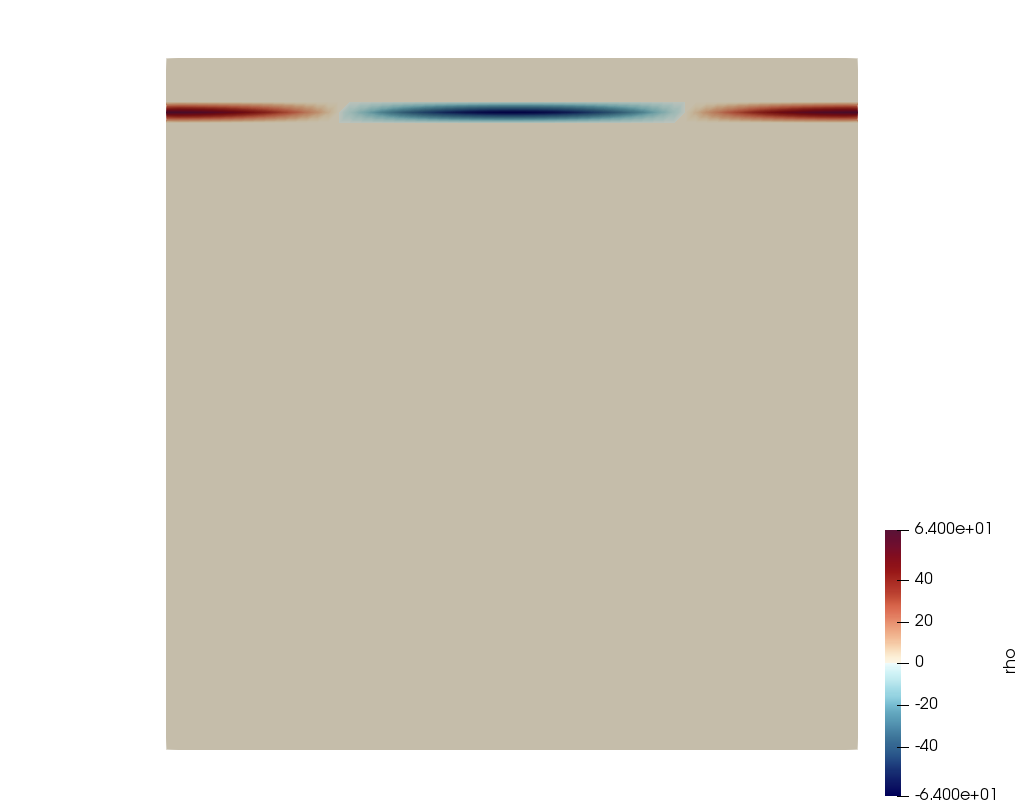
\includegraphics[width=6cm]{python_codes/fieldstone_27/rho}\\
density field for $y_0=59/64$
\end{center}

We choose $\rho \alpha = 64$, $\eta=1$, $g_y=-1$ (note that in this case the 
normalising coefficient of the stress is exactly 1 so it is not implemented).
$\lambda=1$ is set to 1 and we explore $y_0 = \frac{63}{64},\frac{62}{64},\frac{59}{64}$.
Zhong et al. report the following measurements
\footnote{The paper says 60/64 in the last column but it is in fact 59/64}
 at $x=0$:

\begin{center}
\begin{tabular}{l||lll}
\hline
Method             & $y_0=63/64$ & $y_0=62/64$ &  $y_0=59/64$ \\ 
\hline
\hline
Analytic solution                   & 0.995476 & 0.983053  &  0.912506 \\
Pressure smoothing                  & 1.15974  & 1.06498   &  0.911109 \\
CBF                                 & 0.994236 & 0.982116  &  0.912157 \\
\hline
fieldstone: elemental               & 0.824554 & 0.978744  & 0.909574 \\
fieldstone: nodal (C$\rightarrow$N) & 0.824554 & 0.978744  & 0.909574 \\
\hline
\end{tabular}
\end{center}

The $yy$ component of the stress tensor is simply given by
\[
\sigma_{yy} = -p + 2 \eta \dot{\epsilon}_{yy}
\]
and we start with trivial measurements in the elements 
forming the top row of the mesh (pressure is by definition elemental, and strain rate
components are computed in the middle of each element). 

\begin{center}
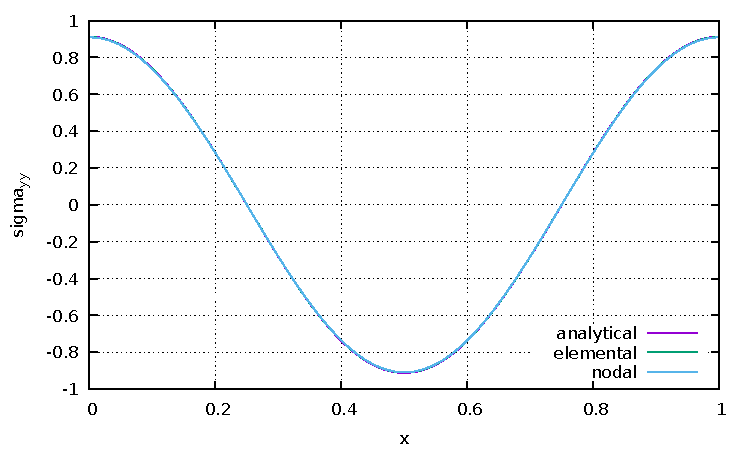
\includegraphics[width=5cm]{python_codes/fieldstone_27/results/59_64/sigmazz.pdf}
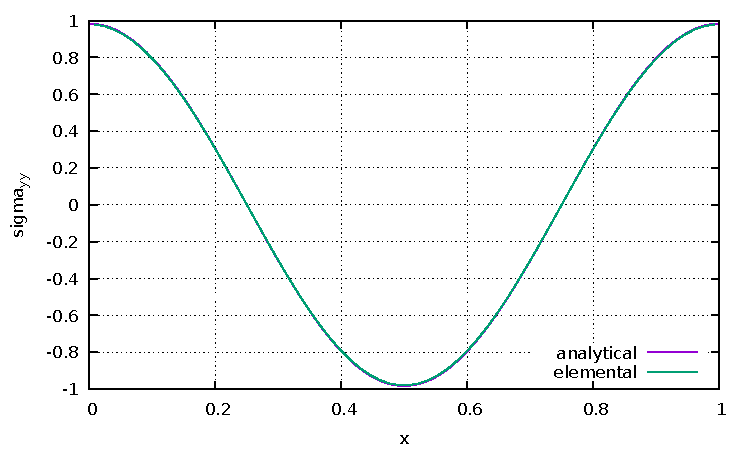
\includegraphics[width=5cm]{python_codes/fieldstone_27/results/62_64/sigmazz.pdf}
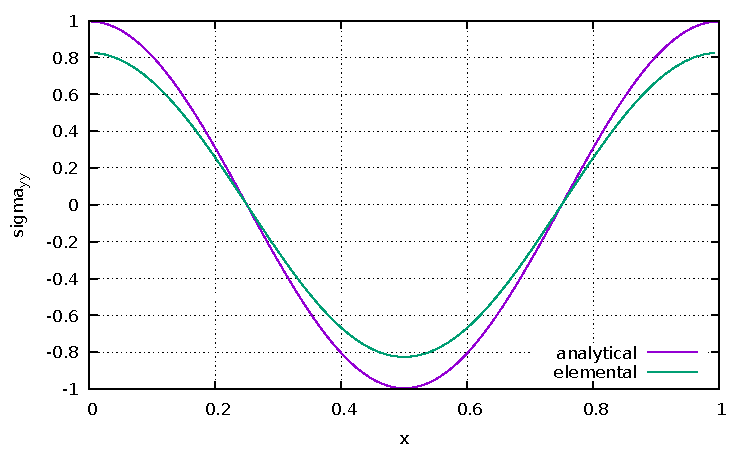
\includegraphics[width=5cm]{python_codes/fieldstone_27/results/63_64/sigmazz.pdf}
\end{center}






\fbox{
\parbox{10cm}{{\bf features}
\begin{itemize}
\item $Q_1\times P_0$ element \index{$Q_1 \times P_0$}
\item incompressible flow \index{incompressible flow}
\item mixed formulation \index{mixed formulation}
\item isothermal \index{isothermal}
\item isoviscous \index{isoviscous}
\item analytical solution \index{analytical solution}
\item pressure smoothing \index{pressure smoothing} 
\item consistent boundary flux \index{CBF}
\end{itemize}
}}



\newpage
%%%%%%%%%%%%%%%%%%%%%%%%%%%%%%%%%%%%%%%%%%%%%%%%%%%%%%%%%%%%%%%%%%%%%%%%%%%%%%%
\section{{\tt fieldstone\_28}: convection 2D box - Tosi et al, 2015 \label{f28}}

The viscosity
field $\mu$ is calculated as the harmonic average between a linear part $\mu_{lin}$ 
that depends on
temperature only or on temperature and depth $d$ , and a non-linear,
plastic part $\mu_{plast}$ dependent on the strain rate:

\begin{equation}
\mu(T,z,\dot{\boldsymbol{\epsilon}}) = 
2 \left(\frac{1}{\mu_\text{lin}(T,z)} + \frac{1}{\mu_\text{plast}(\dot{\boldsymbol{\epsilon}})} \right)^{-1}. 
\label{eq:mu}
\end{equation}

The linear part is given by the linearized Arrhenius law (the so-called Frank-Kamenetskii approximation \cite{frank1969}):

\begin{equation}
\mu_\text{lin} (T,z) = \exp(-\gamma_T T + \gamma_{z} z), \label{eq:mu_Ty}
\end{equation}

where $\gamma_T = \ln ( \Delta\mu_T)$ and $\gamma_{z} = \ln ( \Delta\mu_{z})$ are parameters controlling the total viscosity 
contrast due to temperature ($\Delta\mu_T$) and pressure ($\Delta\mu_{z}$). The non-linear part is given by \cite{trompert1998}: 

\begin{equation}
\mu_\text{plast} (\dot{\boldsymbol{\epsilon}}) = \mu^{*} + \frac{\sigma_Y}{\sqrt{\dot{\boldsymbol{\epsilon}}:\dot{\boldsymbol{\epsilon}}}}, \label{eq:mu_sigma}
\end{equation}

where $\mu^*$ is a constant representing the effective viscosity at high stresses \cite{stein2014b} and $\sigma_Y$ is the yield stress, also assumed to be constant. In 2-D, the denominator in the second term of equation (\ref{eq:mu_sigma}) is given explicitly by

\begin{equation}
\sqrt{\dot{\boldsymbol{\epsilon}}:\dot{\boldsymbol{\epsilon}}} 
= \sqrt{\dot{\epsilon}_{ij} \dot{\epsilon}_{ij} } \\
 = \sqrt{\left( \frac{\partial u_x}{\partial x} \right)^2 + \frac{1}{2} \left( \frac{\partial u_x}{\partial y} 
+ \frac{\partial u_y}{\partial x} \right)^2 + \left( \frac{\partial u_y}{\partial y} \right)^2  }.
\end{equation}

The viscoplastic flow law (equation \ref{eq:mu}) leads to linear viscous deformation at low stresses (equation (\ref{eq:mu_Ty})) and to plastic deformation for stresses that exceed $\sigma_Y$ (equation (\ref{eq:mu_sigma})), with the decrease in viscosity limited by the choice of $\mu^{*}$ \cite{stein2014b}.


In all cases that we present, the domain is a two-dimensional square box. The mechanical boundary conditions are for all boundaries free-slip with no flux across, i.e. $\tau_{xy}=\tau_{yx}=0$ and $\boldsymbol{u}\cdot \boldsymbol{n}=0$, where $\boldsymbol{n}$ denotes the outward normal to the boundary. Concerning the energy equation, the bottom and top boundaries are isothermal, with the temperature $T$ set to 1 and 0, respectively, while side-walls are assumed to be insulating, i.e. $\partial T/\partial x = 0$. The initial distribution of the temperature field is prescribed as follows:

\begin{equation}
T(x,y) = (1-y) + A \cos(\pi x)\sin(\pi y), \label{eq:initemp}
\end{equation}
where $A=0.01$ is the amplitude of the initial perturbation.


In the following Table \ref{tab:bench_cases}, we list the benchmark cases according to the parameters used. 


\begin{center}
\begin{tabular}{c c c c c c c} 
\hline
Case & $Ra$ & $\Delta\mu_T$ & $\Delta\mu_y$ & $\mu^*$ & $\sigma_Y$ & Convective regime \\
\hline
1   & $10^2$ & $10^5$    & 1  & -- & --             & Stagnant lid    \\
2   & $10^2$ & $10^5$    & 1  & $10^{-3}$ & 1       & Mobile lid \\
3   & $10^2$ & $10^5$    & 10 & --  & --            & Stagnant lid \\
4   & $10^2$ & $10^5$    & 10 & $10^{-3}$ & 1       & Mobile lid  \\
5a  & $10^2$ & $10^5$    & 10 & $10^{-3}$ & 4       & Periodic  \\
5b  & $10^2$ & $10^5$    & 10 & $10^{-3}$ & 3 -- 5  & Mobile lid -- Periodic -- Stagnant lid \\
\hline
\end{tabular}\\
{\small Benchmark cases and corresponding parameters.} 
\end{center}

In Cases 1 and 3 the viscosity is directly calculated from equation (\ref{eq:mu_Ty}), while for Cases 2, 4, 5a, and 5b, we used equation (\ref{eq:mu}). For a given mesh resolution, Case 5b requires running simulations with yield stress varying between 3 and 5


In all tests, the reference Rayleigh number is set at the surface ($y=1$) to $10^2$, and the viscosity contrast due to temperature $\Delta\mu_T$ is $10^5$, implying therefore a maximum effective Rayleigh number of $10^7$ for $T=1$. Cases 3, 4, 5a, and 5b employ in addition a depth-dependent rheology with viscosity contrast  $\Delta\mu_z=10$. Cases 1 and 3 assume a linear viscous rheology that leads to a stagnant lid regime. Cases 2 and 4 assume a viscoplastic rheology that leads instead to a mobile lid regime. Case 5a also assumes a viscoplastic rheology but a higher yield stress, which ultimately causes the emergence of a strictly periodic regime. The setup of Case 5b is identical to that of Case 5a but the test consists in running several simulations using different yield stresses. Specifically, we varied $\sigma_Y$ between 3 and 5 in increments of 0.1 in order to identify the values of the yield stress corresponding to the transition from mobile to periodic and from periodic to stagnant lid regime. 

\newpage
\subsubsection{Case 0: Newtonian case, a la Blankenbach et al., 1989}

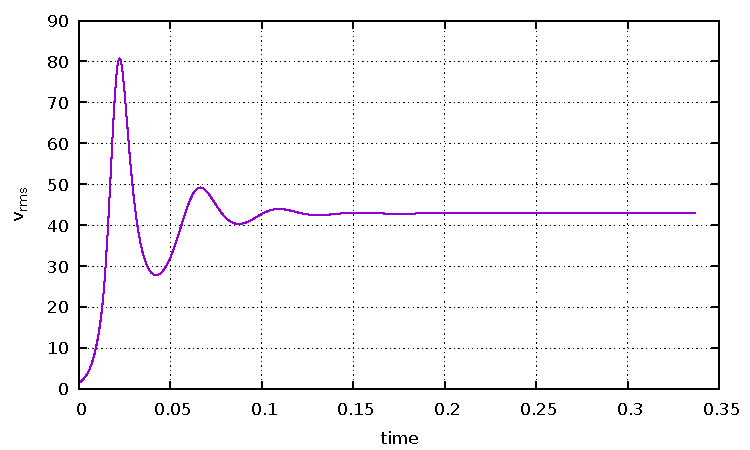
\includegraphics[width=5cm]{python_codes/fieldstone_28/results_case0/vrms.pdf}
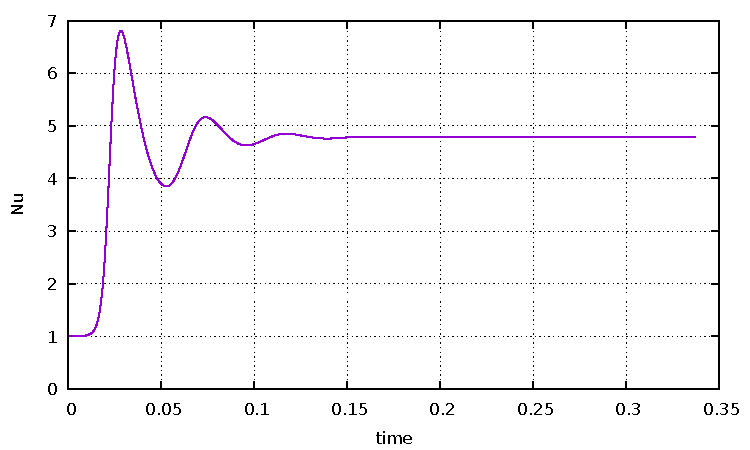
\includegraphics[width=5cm]{python_codes/fieldstone_28/results_case0/Nu.pdf}
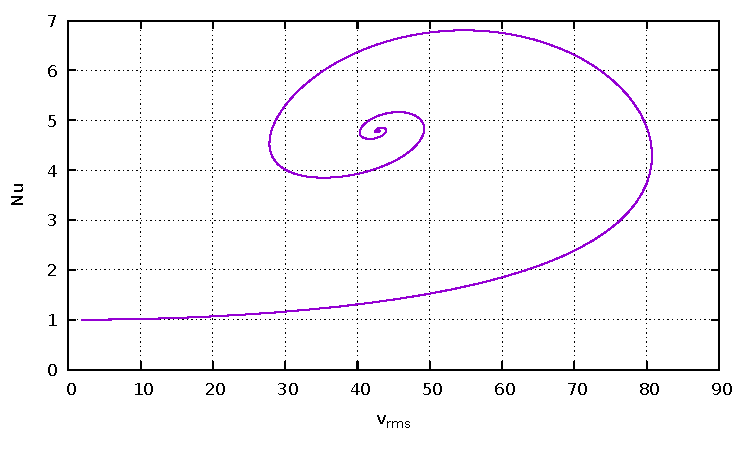
\includegraphics[width=5cm]{python_codes/fieldstone_28/results_case0/vrms_Nu.pdf}

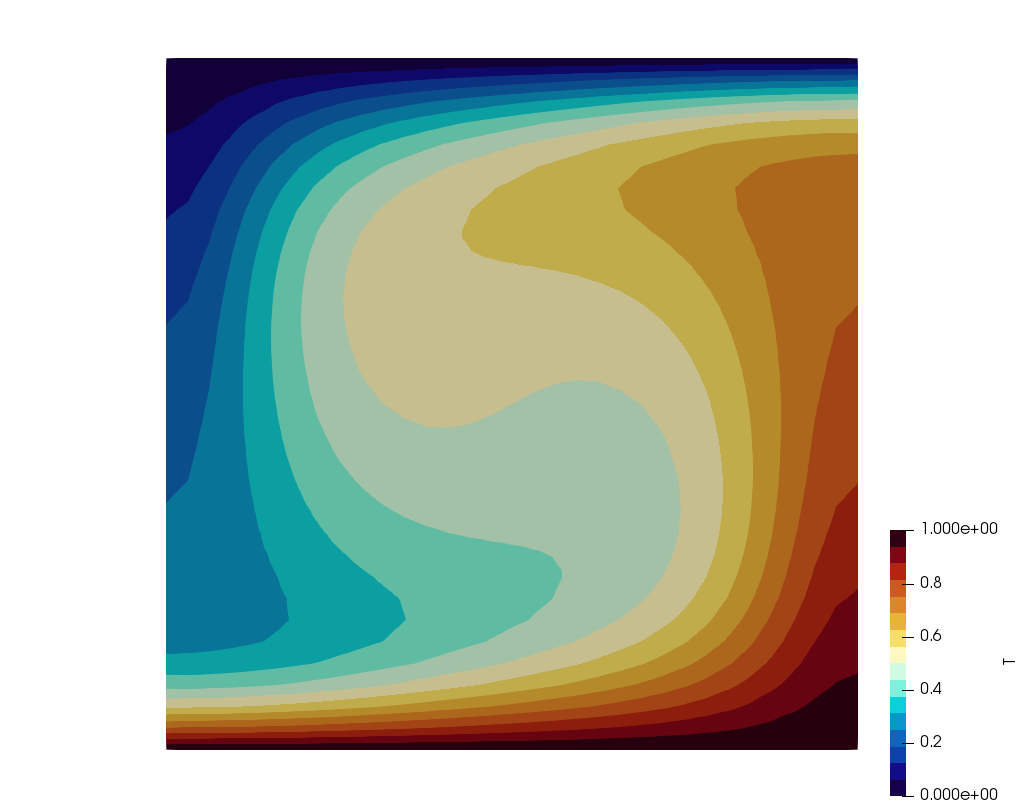
\includegraphics[width=5cm]{python_codes/fieldstone_28/results_case0/temp}
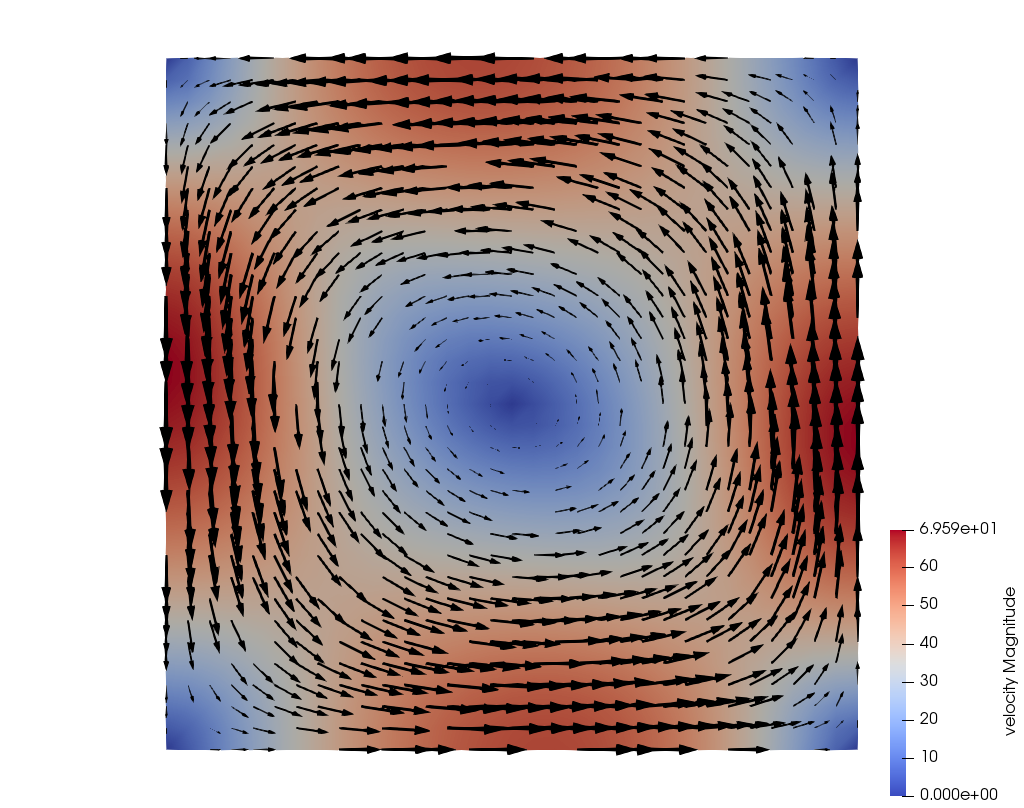
\includegraphics[width=5cm]{python_codes/fieldstone_28/results_case0/vel}



\newpage %-------------------------------------------------------
\subsubsection{Case 1}

In this case $\mu^\star=0$ and $\sigma_Y=0$ so that $\mu_{plast}$ can be discarded.
The CFL number is set to 0.5 and the viscosity is given by 
$\mu(T,z,\dot{\boldsymbol{\epsilon}}) =   \mu_\text{lin}(T,z) $.
And since $\Delta \mu_z=1$ then $\gamma_z=0$ so that
$\mu_\text{lin} (T,z) = \exp(-\gamma_T T )$

\begin{center}
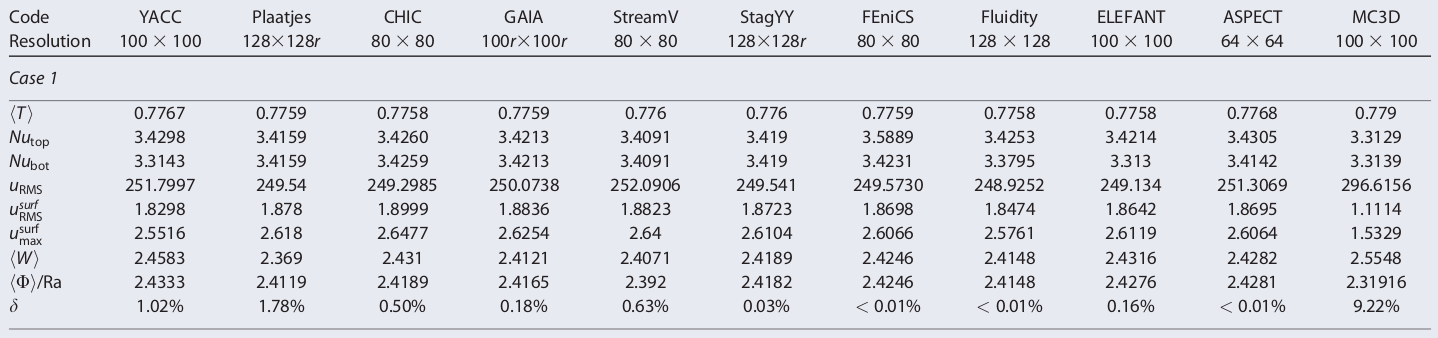
\includegraphics[width=15cm]{python_codes/fieldstone_28/results_case1/tosn15b}\\
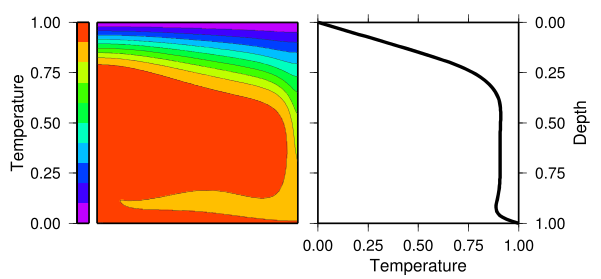
\includegraphics[width=5cm]{python_codes/fieldstone_28/results_case1/tosn15a1}
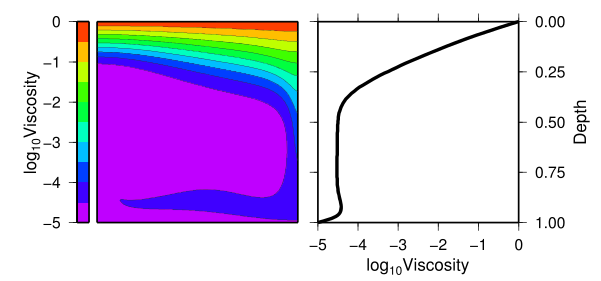
\includegraphics[width=5cm]{python_codes/fieldstone_28/results_case1/tosn15a2}
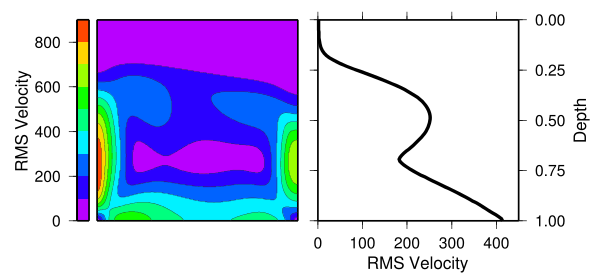
\includegraphics[width=5cm]{python_codes/fieldstone_28/results_case1/tosn15a3}
\end{center}
\begin{center}
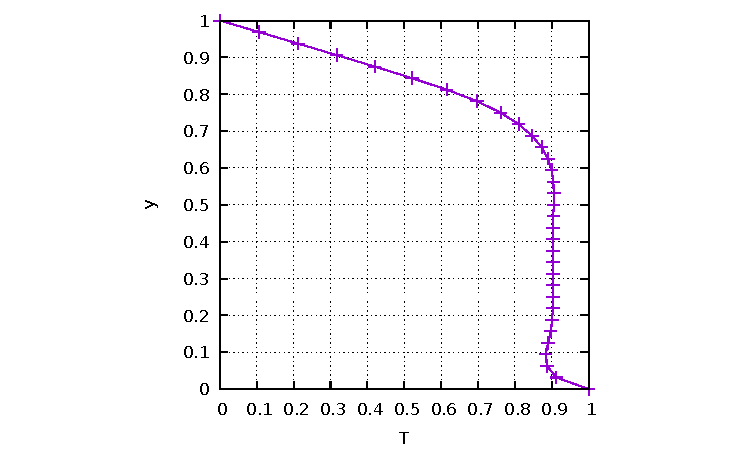
\includegraphics[width=5cm]{python_codes/fieldstone_28/results_case1/T_profile.pdf}
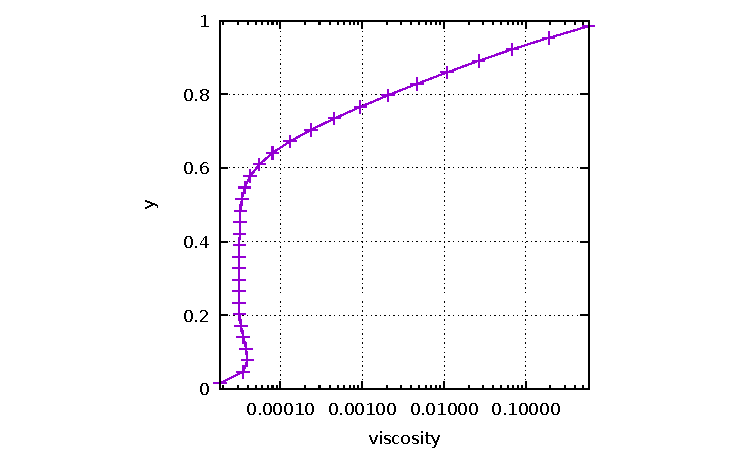
\includegraphics[width=5cm]{python_codes/fieldstone_28/results_case1/eta_profile.pdf}
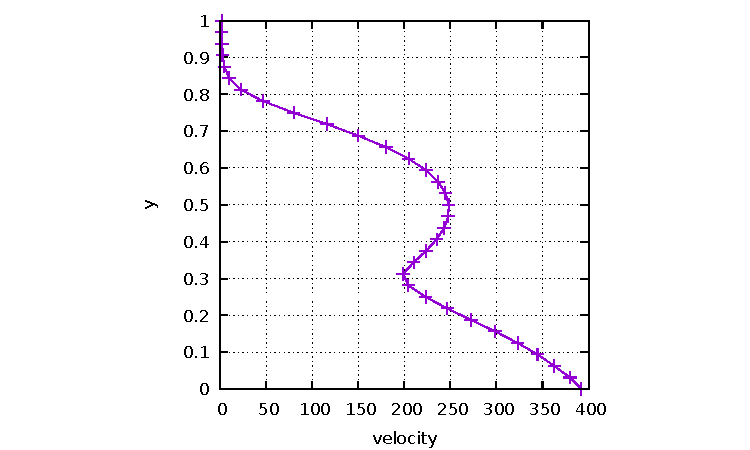
\includegraphics[width=5cm]{python_codes/fieldstone_28/results_case1/V_profile.pdf}
\end{center}


\begin{center}
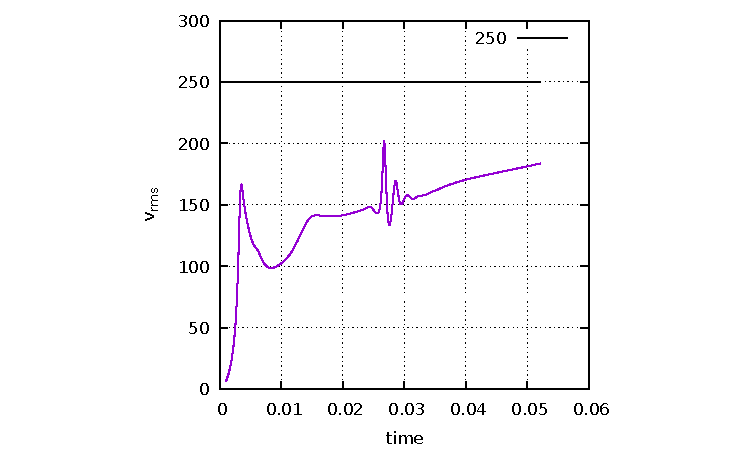
\includegraphics[width=7cm]{python_codes/fieldstone_28/results_case1/vrms.pdf}
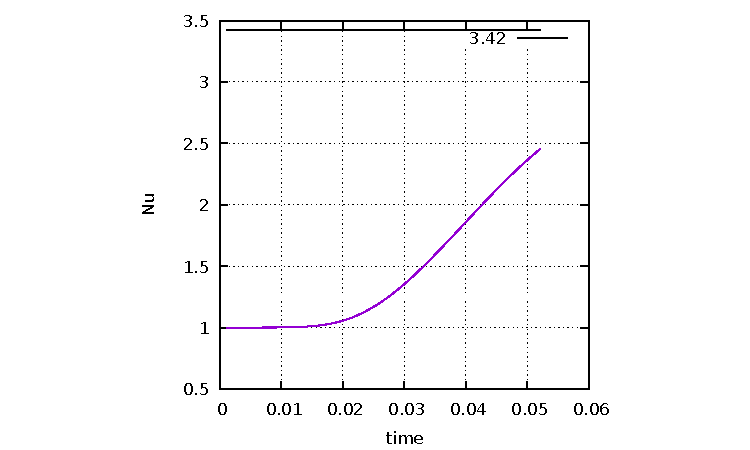
\includegraphics[width=7cm]{python_codes/fieldstone_28/results_case1/Nu.pdf}\\
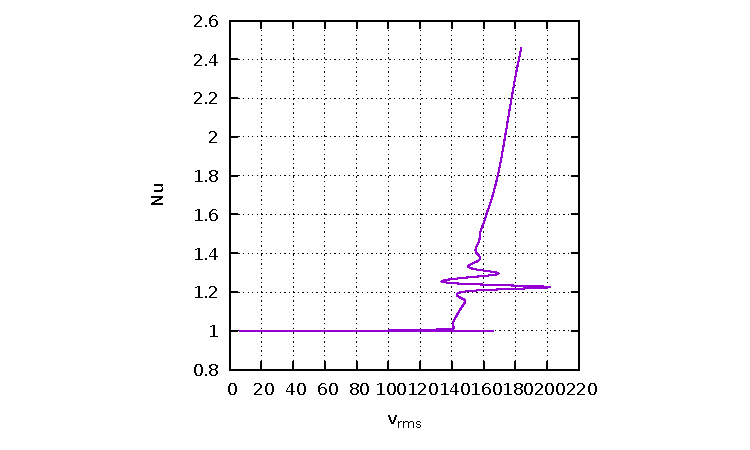
\includegraphics[width=7cm]{python_codes/fieldstone_28/results_case1/vrms_Nu.pdf}
\includegraphics[width=7cm]{python_codes/fieldstone_28/results_case1/Tavrg.pdf}
\end{center}











\newpage
%%%%%%%%%%%%%%%%%%%%%%%%%%%%%%%%%%%%%%%%%%%%%%%%%%%%%%%%%%%%%%%%%%%%%%%%%%%%%%%
\section{{\tt fieldstone}: Gravity: buried sphere}
The details of the numerical setup are presented in Section \ref{f1}.

Each element has $m_V=16$ vertices so in total $ndof_V\times m_V=32$ 
velocity dofs and 
$ndof_P*m_P=9$ pressure dofs. The total number of 
velocity dofs is therefore $NfemV=nnp \times ndofV$ while the total number of
pressure dofs is $NfemP=nel$. The total number of dofs is then $Nfem=NfemV+NfemP$.

As a consequence, matrix $\K$ has size $NfemV,NfemV$ and matrix $\G$ has size $NfemV,NfemP$.
Vector $f$ is of size $NfemV$ and vector $h$ is of size $NfemP$.  

\begin{verbatim}

60===61===62===63===64===65===66===67===68===70
||             ||             ||             ||
50   51   52   53   54   55   56   57   58   59
||             ||             ||             ||
40   41   42   43   44   45   46   47   48   49
||             ||             ||             ||
30===31===32===33===34===35===36===37===38===39
||             ||             ||             ||
20   21   22   23   24   25   26   27   28   29
||             ||             ||             ||
10   11   12   13   14   15   16   17   18   19
||             ||             ||             ||
00===01===02===03===04===05===06===07===08===09

Example of 3x2 mesh. nnx=10, nny=7, nnp=70, nelx=3, nely=2, nel=6
\end{verbatim}


\begin{verbatim}
12===13===14===15           06=====07=====08
||   ||   ||   ||           ||     ||     ||
08===09===10===11           ||     ||     ||
||   ||   ||   ||           03=====04=====05
04===05===06===07           ||     ||     ||
||   ||   ||   ||           ||     ||     ||
00===01===02===03           00=====01=====02

Velocity (Q3)               Pressure (Q2)

(r,s)_{00}=(-1,-1)          (r,s)_{00}=(-1,-1) 
(r,s)_{01}=(-1/3,-1)        (r,s)_{01}=(0,-1) 
(r,s)_{02}=(+1/3,-1)        (r,s)_{02}=(+1,-1) 
(r,s)_{03}=(+1,-1)          (r,s)_{03}=(-1,0) 
(r,s)_{04}=(-1,-1/3)        (r,s)_{04}=(0,0) 
(r,s)_{05}=(-1/3,-1/3)      (r,s)_{05}=(+1,0) 
(r,s)_{06}=(+1/3,-1/3)      (r,s)_{06}=(-1,+1) 
(r,s)_{07}=(+1,-1/3)        (r,s)_{07}=(0,+1) 
(r,s)_{08}=(-1,+1/3)        (r,s)_{08}=(+1,+1) 
(r,s)_{09}=(-1/3,+1/3)
(r,s)_{10}=(+1/3,+1/3)
(r,s)_{11}=(+1,+1/3)
(r,s)_{12}=(-1,+1)
(r,s)_{13}=(-1/3,+1)
(r,s)_{14}=(+1/3,+1)
(r,s)_{15}=(+1,+1)

\end{verbatim}







{\color{red} Write about 4 point quadrature}.








\fbox{
\parbox{10cm}{{\bf features}
\begin{itemize}
\item $Q_3\times Q_2$ element \index{$Q_3 \times Q_2$}
\item incompressible flow \index{incompressible flow}
\item mixed formulation \index{mixed formulation}
\item isothermal \index{isothermal}
\item isoviscous \index{isoviscous}
\item analytical solution \index{analytical solution}
\end{itemize}
}}

\begin{center}
\includegraphics[width=10cm]{python_codes/fieldstone_19/errors}
\end{center}

velocity error rate is cubic, pressure superconvergent since the pressure field
is quadratic and therefore lies into the Q2 space.


\appendix

\newpage
%%%%%%%%%%%%%%%%%%%%%%%%%%%%%%%%%%%%%%%%%%%%%%%%%%%%%%%%%%%%%%%%%%%%%%%%%%%%%%%
%\section{The main codes in computational geodynamics}
%\input{codes}

\newpage %---------------------------------------------------------------------
\bibliographystyle{plain} %----------------------------------------------------
\bibliography{../../writings/biblio_geosciences2} %----------------------------

\printindex %------------------------------------------------------------------

\newpage %---------------------------------------------------------------------
\listoftodos[Notes] %----------------------------------------------------------

\end{document}


%%%%%%%%%%%%%%%%%%%%%%%%%%%%%%%%%%%%%%%%%%%%%%%%%%%%%%%%%%%%%%%%%%%%%%%%%%%%%%%
%\section{fieldstone.py}
%\lstinputlisting{python_codes/fieldstone/fieldstone.py}
